% Tento soubor nahraďte vlastním souborem s obsahem práce.
%=========================================================================
% Autoři: Michal Bidlo, Bohuslav Křena, Jaroslav Dytrych, Petr Veigend a Adam Herout 2019

% Pro kompilaci po částech (viz projekt.tex), nutno odkomentovat a upravit
%\documentclass[../projekt.tex]{subfiles}
%\begin{document}

%===---------------====
% UVOD
%===---------------====
\chapter{Úvod}
Tato bakalářská práce má za cíl vytvořit automatický způsob generování 2D bludišť různých velikostí za pomoci celulárních automatů a dalších algoritmů. Program vytvářející tyto bludiště je následně využit ve hře zaměřující se na procházení labyrintů.

Téma generování bludišť pomocí celulárních automatů patří do oblasti herního designu a vývoje. Konkrétněji do odvětví procedurálního generování, jenž se v herním průmyslu využívá k automatickému vytváření různorodých herních prostředí/úrovní. 

Procedurální generování je v dnešní době čím dál populárnější. Jeho implementací se zlepšuje rozmanitost a znovu-hratelnost her, což přináší hráčům nové výzvy při prozkoumávání prostředí. Herním vývojářům to umožňuje soustředit se na důležitější aspekty hry.

Úkolem práce bylo vyvinout způsob, kterým je možno procedurálně generovat bludiště libovolných velikostí. Toho bylo dosaženo pomocí celulárních automatů a dalších technik, jako například grafových algoritmů, či prohledávacích metod. Výsledný algoritmus generování byl následně implementován do hry, jež prezentuje jedno z jeho možných využití. Cílem vytvořené hry je otestování navigačních dovedností hráčů prostřednictvím postupného procházení úrovní, kde každá nabízí unikátní vygenerované bludiště. Hráči čelí nejen fyzickým výzvám v podobě komplexních chodeb, ale také časovému tlaku a boji s nepřáteli. Snímky z výsledné hry (menu a hraná úroveň), je možno vidět na obrázku~\ref{fig:final_game}.

\begin{figure}[b]
    \centering
    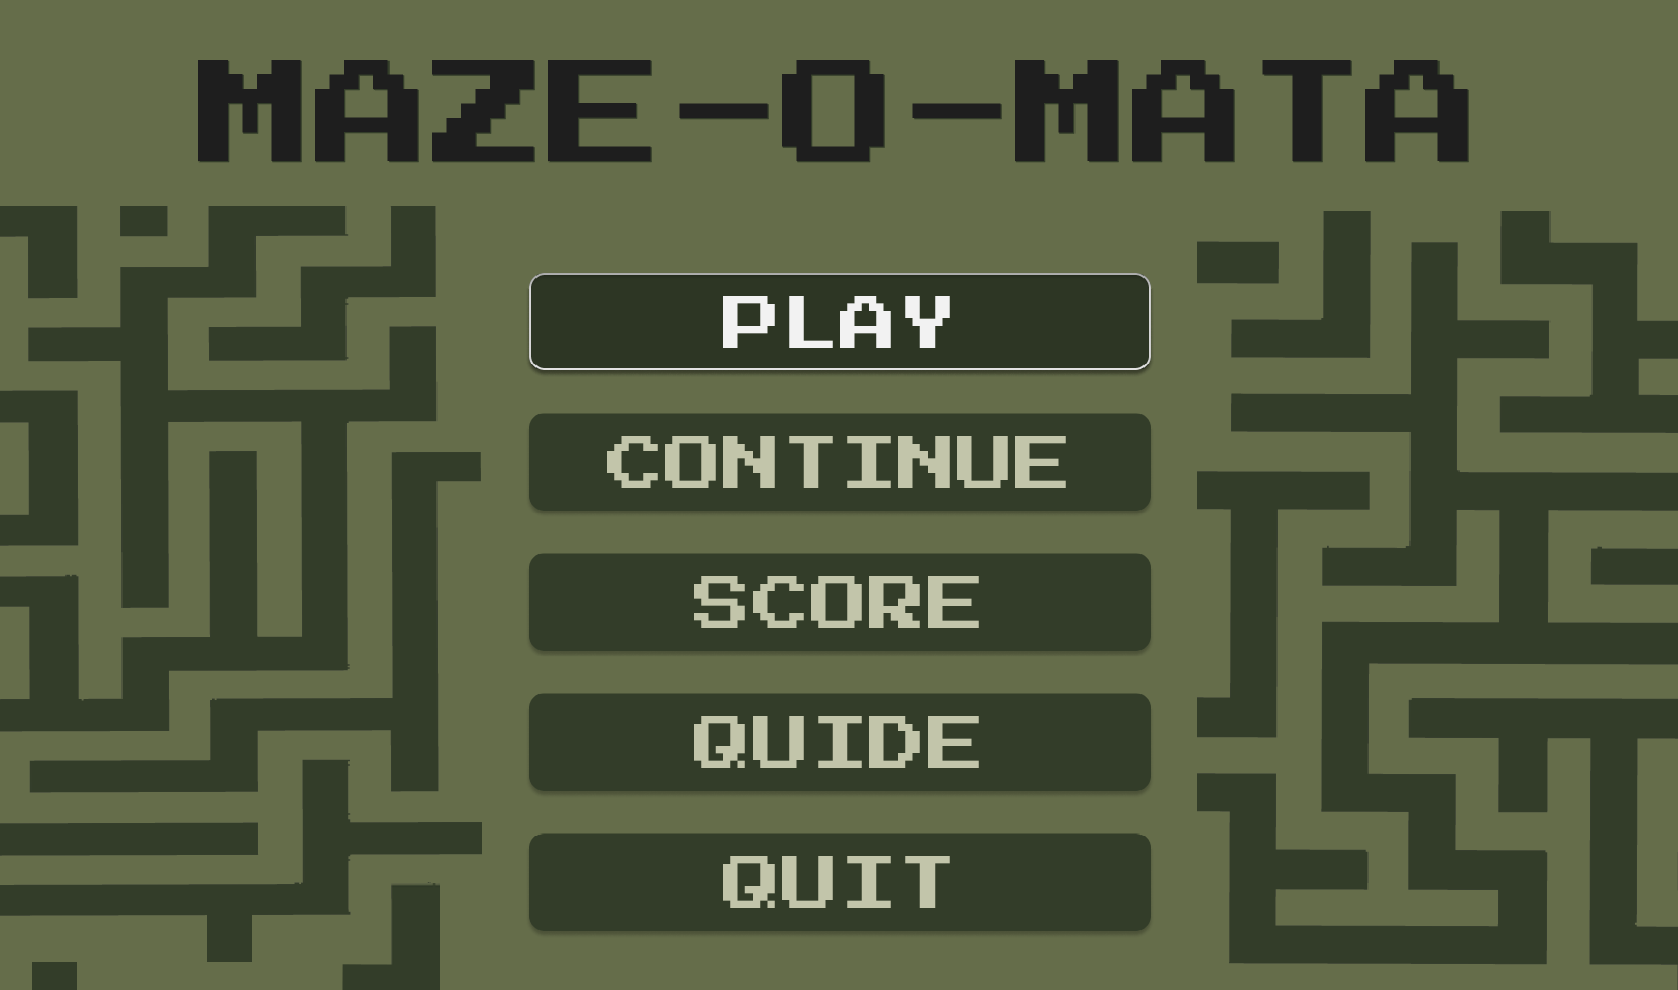
\includegraphics[width=0.45\textwidth]{obrazky-figures/ch1/game_menu.png}\hspace{0.5cm}
    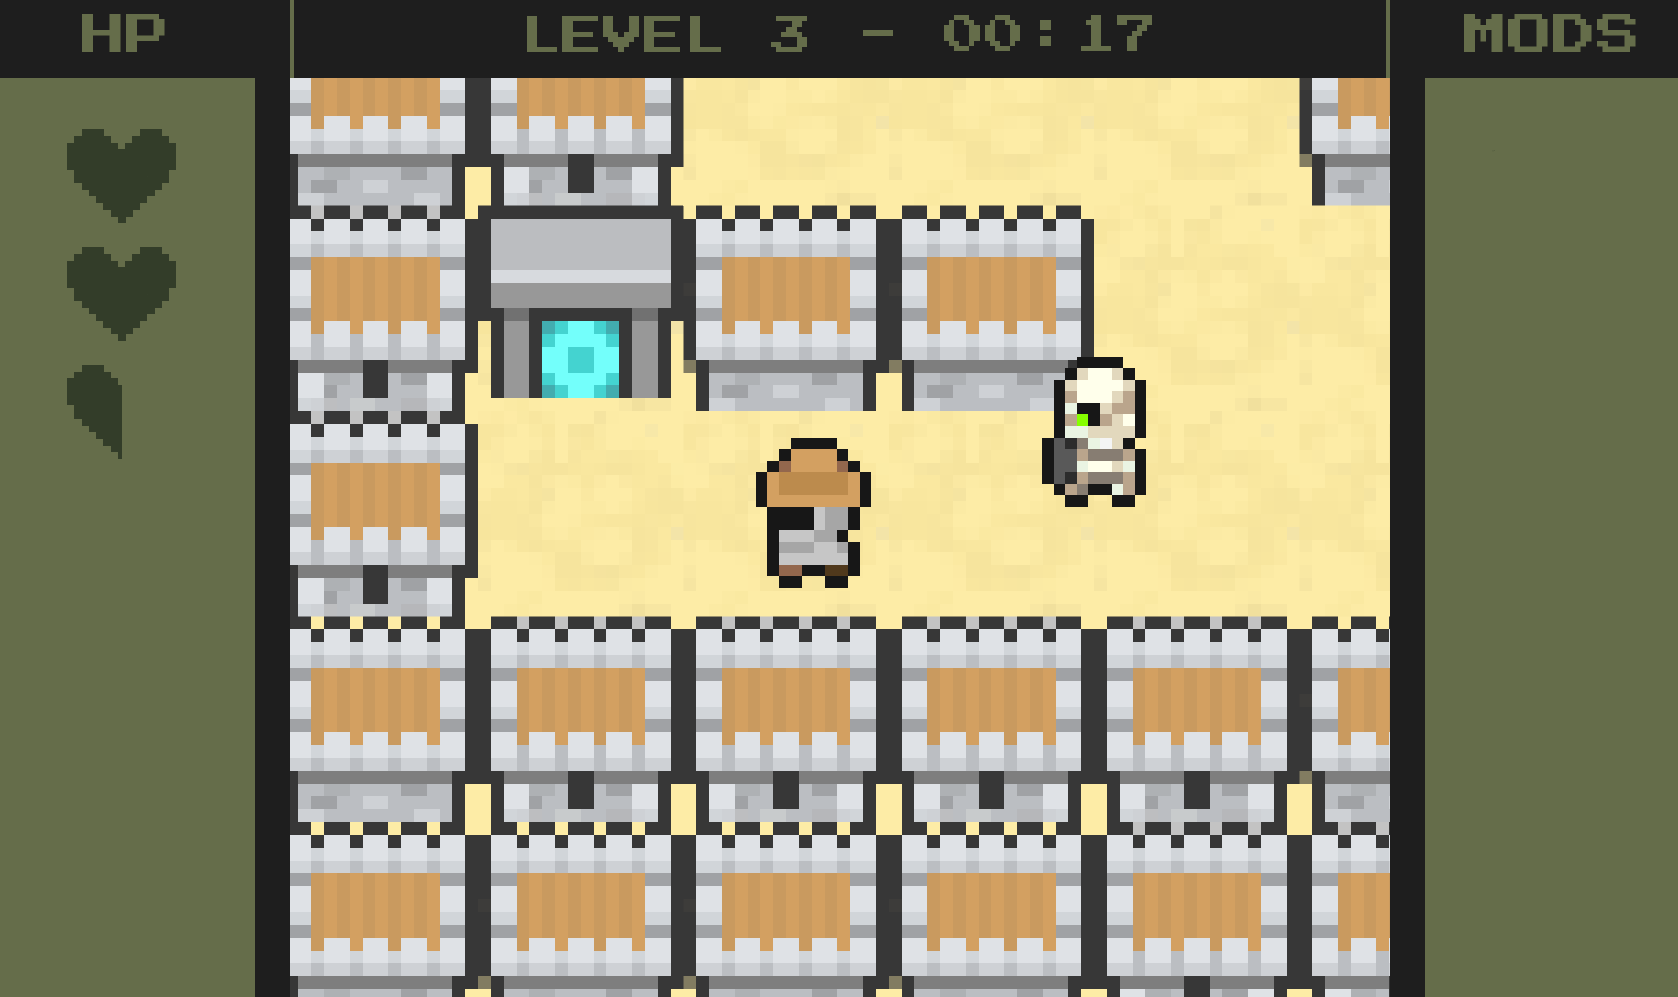
\includegraphics[width=0.45\textwidth]{obrazky-figures/ch1/game_screen.png}
    \caption{Snímky z výsledné hry.}
    \label{fig:final_game}
\end{figure}

Kapitola~\ref{chap:Aspekty vývoje videoher} je věnována průzkumu vývoje videoher, jejich historii a také obsahuje i~detailnější náhled na různé labyrintové hry. V kapitole je popsána také důležitá teorie, jež byla využita k~vytvoření algoritmu generování labyrintů\,--\,například celulární automaty, stavový prostor, či rejection sampling. Následující kapitola~\ref{chap:Koncept 2D labyrintové hry} se věnuje podrobnému návrhu přístupu ke generování bludiště. Zde je možné nalézt popis postupu vývoje hry, návrh herních prvků a~uživatelského rozhraní. V kapitole~\ref{Tvorba bludiště a realizace hry} je popisována implementace jak algoritmu generování labyrintů, tak jeho integrace do finální hry. Nachází se zde také podkapitola věnována testování algoritmu. Cílem tohoto testování bylo nalézt nejoptimálnější způsob generování pro různé velikosti. Po vytvoření alfa verze hry bylo nutné hru nechat otestovat uživateli. Podrobnosti k tomuto uživatelskému testování, kterými je například analýza, či výsledky, se nachází v~kapitole~\ref{chap:Uživatelské testování}. Poslední kapitola~\ref{chap:Závěr} je věnována konečnému zhodnocení výsledků práce.

%===---------------====
% TEORIE
%===---------------====
\chapter{Aspekty vývoje videoher}\label{chap:Aspekty vývoje videoher}
Vývoj videoher je práce, jejímž výsledkem je hra na elektronické zařízení, jako například počítač, telefon, či konzole. Na jejím vzniku spolupracují umělci, designeři a programátoři, kteří mohou využít software vytvořený pro vývoj her\,--\,herní engine. Ten nabízí prostředky pro pohodlnější práci na vývoji her (viz kapitola~\ref{chap:Herní engine} Herní engine).

Proces vývoje videoher lze rozdělit na 7 základních etap: plánování, preprodukce, produkce, testování, prelaunch, spuštění a postprodukce~\cite{g2_game_development}.
\subsection*{Plánování}
V této etapě je vytvářen prvotní nápad na vývoj hry. Je základním kamenem a proto je velmi důležité důkladně vše promyslet a připravit, jelikož pozdější změny v plánu hry mohou mít drtivé dopady na celý vývoj~\cite{GameMaker_development}, jak časové, tak finanční. 

Plánování je celé o pokládání si otázek a jejich zodpovídání. Ty mohou být obecné \uv{Jaký typ hry budeme vytvářet?}, \uv{Kdo bude cílové publikum naší hry?}, nebo se týkat příběhu hry: \uv{Jaká bude zápletka příběhu?}, \uv{Kde se bude hra odehrávat?}, \uv{Jaké postavy se budou ve hře nacházet?} a také technických parametrů hry: \uv{Pro jakou platformu budeme hru vytvářet?}, \uv{Jaké budou klíčové vlastnosti naší hry?}~\cite{g2_game_development}.

Pro takzvaný \uv{proof of concept}, díky kterému je zváženo, zda je možné danou hru vytvořit, je důležité najít a zanalyzovat odpovědi na otázky pro trh~\cite{GameMaker_development}. Těmi jsou například otázky jako \uv{Kolik bude stát vývoj hry a jak tyto peníze získáme?}, \uv{Jak dlouho bude trvat vývoj?}, \uv{Máme potřebné zaměstnance a technologie na vývoj?} či \uv{Jakým způsobem hru zpeněžíme?}.

Cílem plánování je vytvořit základní koncept\,--\,o čem hra bude, zjistit si cílový trh a~zhodnotit firemní zdroje a potenciály~\cite{novak2011game}.

\begin{figure}[hb]
    \centering
	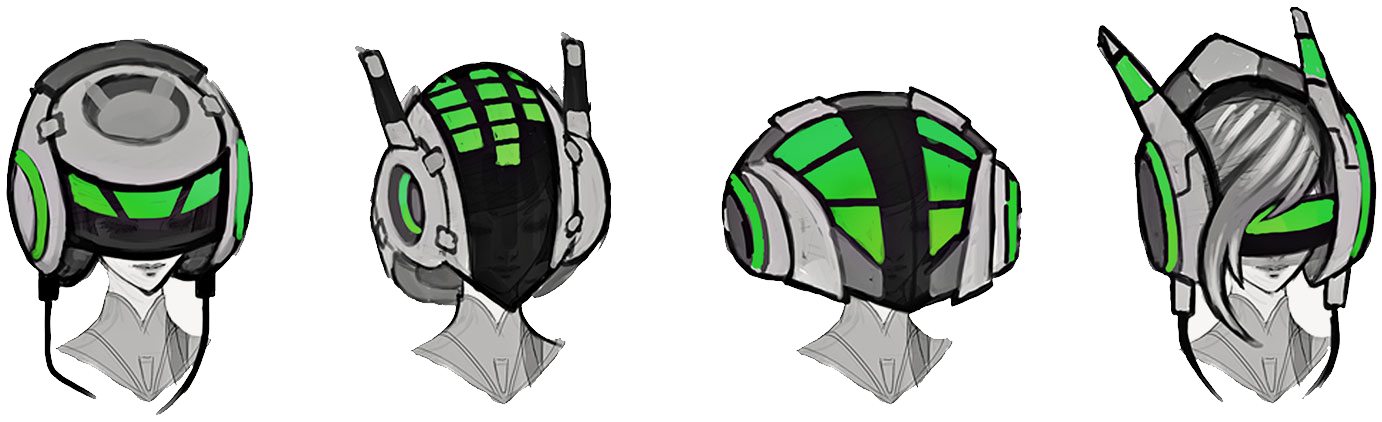
\includegraphics[width=0.85\textwidth]{obrazky-figures/ch2/concept_art.png}
	\caption{Concept art postavy ze hry League of Legends.~\cite{artLOLvol1}}
	\label{fig:concept_art_lol}
\end{figure}

\subsection*{Preprodukce}
Tato fáze přebírá odpovědi z plánování a rozšiřuje je o důležité detaily. Odehrává se při ní mnoho kooperací mezi různými týmy (spisovatelé, programátoři, umělci, designeři, ...), aby se vyhovělo co nejvíce požadavkům a zabránilo se pozdějším komplikacím. Programátoři například spisovatelům přiblíží technologické překážky platformy, které není možné překročit, či umělci a designeři navrhnou konzistentní barevné palety~\cite{g2_game_development}.

Výsledkem preprodukce je dokument o herním designu (\textit{Game Design Document}, neboli GDD) a dokument technického návrhu a mohou zde být navrhovány první prototypy~\cite{novak2011game}. GDD je \uv{živý} dokument a vyvíjí se postupně po celou tvorbu hry\,--\,nalezneme tam detailní popis věcí, jako například myšlenku hry, její žánr, celkový příběh, strategii monetizace, informace o postavách, základní herní mechaniky, design úrovní a světa, skici a \textit{concept arty}, neboli návrhy objektů/prostředí/postav~\cite{CG_Spectrum_GAMEDEVELOPMENT} (ukázka concept artu je na obrázku~\ref{fig:concept_art_lol}).

\subsection*{Produkce}
Nejdelší, nejdražší, nejnáročnější a nejdůležitější část vývoje~\cite{g2_game_development}, jejímž výsledkem je hotová hra. 

V této fázi je postupně vytvářen finální produkt. Jsou vymodelovány a animovány objekty, jako jsou postavy, či prostředí. Ty  jsou dále naprogramovány, čímž se přidají herní mechaniky a objekty jsou přivedeny k životu~\cite{GameMaker_development}. Tomu napomáhají i zvukoví designéři~a~dabéři, kteří se starají o audio stránku hry.

Při produkci nejsou neobvyklé změny, při kterých je nutné smazat i celé segmenty hry~\cite{g2_game_development}. Často se stává, že je nutné změnit nějaké navržené či již vytvořené části, ať už je to kvůli nutnosti zmenšit pracovní zátěž vývojářského týmu, či kvůli zjištění, že neimplementovaný objekt do hry nesedí, či nefunguje podle původních představ. Příkladem je postava \uv{Boatman} ze hry Spyro the Dragon (viz obrázek~\ref{fig:spyro_cut}), která byla změněna na postavu \uv{Ballonist}, nejspíše aby dávalo větší smysl cestování na ostrov v oblacích~\cite{GameMaker_development}.

\begin{figure}[hb]
    \vspace{0.5cm}
    \centering
    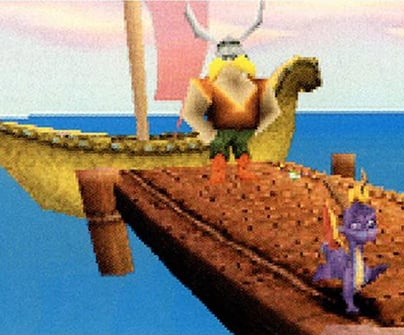
\includegraphics[width=0.5\textwidth]{obrazky-figures/ch2/Spyro-Boatman.png}\hspace{0.1cm}
    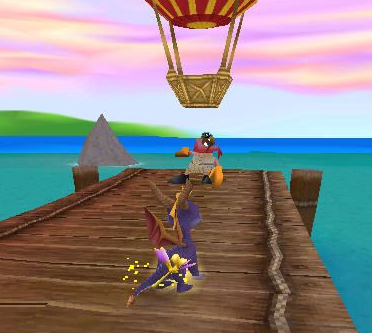
\includegraphics[width=0.46\textwidth]{obrazky-figures/ch2/Spyro-Ballonist.png}
    \caption{Postava jménem Boatman (vlevo) ze hry Spyro the Dragon, která byla ve finální hře změněna na postavu jménem Ballonist (vpravo).~\cite{GameMaker_development}}
    \label{fig:spyro_cut}
\end{figure}

\subsection*{Testování}
Další důležitou fází je testování. V této fázi je důležité otestovat všechny možné problémy hry, které by mohli kazit zážitek ze hry.

Testy se dají rozdělit na 2 základní typy\,--\,testy technické stability a testování takzvaného \uv{fun factoru} hry, což je průzkum hratelnosti hry, její zábavnosti, poutavosti, a nebo zda není moc těžká, či lehká~\cite{GameMaker_development}. Testy technického faktoru zkoumají, zda se hra správně renderuje a neseká se. Dále testeři vyhledávají různé bugy/chyby (např. zda opravdu nejde projít zdmi, nebo jestli se postavička projde místy, kterými by měla v pořádku projít), testují, zda všechny funkce a postavy fungují dle specifikací a další podobné věci~\cite{g2_game_development}.

\subsection*{Prelaunch}
Fáze před publikací je marketingová. Je to období kdy se k veřejnosti dostávají trailery, teasery a demo verze hry~\cite{GameMaker_development}. Díky tomu může hra získat větší fanouškovskou základnu a~vydavatel může získat první zpětnou vazbu od veřejnosti.

\subsection*{Publikace}
V této fázi dochází k vypuštění a distribuci plné verze hry publiku.

Do spuštění hry musí být opraveno co nejvíce chyb (nejlépe všechny), proto často studia přichází s hierarchií chyb, které jsou potřeba opravit. Od těch nejproblémovějších, které například způsobují pády hry, až po ty nejdrobnější~\cite{g2_game_development}.

\subsection*{Postprodukce}
V této etapě již hru může koupit a hrát zákazník. Obvykle  jsou také vydávány bezplatné aktualizace (zvané \textit{patch}), které ji technicky vylepšují, vyvažují a často i opravují chyby~\cite{novak2011game}, na které se nedostalo při produkci, či které byly nově objeveny hráči. 

V této fázi také mohou být vydávány i aktualizace, které do hry přidávají nový obsah (například události, nové postavy/místa atd.)~\cite{g2_game_development}. Tyto aktualizace jsou však často přidávány formou rozšíření/datadisků neboli DLC. Ty jsou oproti běžným aktualizacím obvykle placené, nabízí více obsahu a pro jejich spuštění vyžadují standardně originální hru (v některých případech ale figurují i jako samostatná hra)~\cite{novak2011game}. Nový obsah udržuje hru relevantní~\cite{GameMaker_development}.

\subsection*{Milníky verzí vývoje her}
V průběhu vývoje videohra projde několika různými verzemi, které se od sebe odlišují jejich technickými vlastnostmi. Kniha Game Development Essentials: An Introduction~\cite{novak2011game} uvádí nejdůležitější 3 z nich uvedené níže.
\begin{itemize}
    \item Alfa\,--\,v této fázi je již hra hratelná od začátku k cíli a je označována jako \textit{\uv{feature complete}}~\cite{CG_Spectrum_GAMEDEVELOPMENT}, což znamená že všechny hlavní vlastnosti jsou již implementované, nemusí zde být ale vše kompletně zoptimalizované. Měla by to být první verze testovaná lidmi mimo vývojářský tým.
    \item Beta\,--\,hra již v sobě má integrovaný všechen obsah, zaměření už primárně na opravu chyb a stabilizaci.
    \item Gold\,--\,finální dodělaná hra, která je připravena pro publikaci.
\end{itemize}

%--------------------------
% Počátek videoher
\section{Počátek videoher}
První počítačové hry vznikaly kolem 50. let 20. století v prostředí vojenských základen a univerzit na jejich sálových počítačích~\cite{novak2011game}. Těmi byly například videohry OXO (1952) a Tennis for Two (1958), ale mezi nejpopulárnější videohry (vytvořené v té době) se počítá především hra Spacewar!~\cite{bellis2019spacewar}. Ta byla vytvořena studentem univerzity MIT, Stevem Russellem a lze ji vidět na obrázku~\ref{fig:spacewar}. 


Nápad této hry byl následně na začátku 70. let přebrán Nolanem Bushnellem (zakladatelem Atari), který z ní vytvořil první komerční arkádovou hru (a tedy volně přístupnou veřejnosti) pod jménem \uv{Computer Space}, která byla velmi úspěšná~\cite{video_games_history}. To spustilo vývoj dalších úspěšných arkádových videoher, oproti dnešním hrám převážně dovednostních. Příkladem mohou být hry \uv{Pong}, či \uv{Space Invaders} a \uv{Asteroids}, což byly první hry umožňující ukládání skóre, dále například Galaxian, Pac-Man, Donkey Kong a Tron~\cite{novak2011game}.

Ve stejnou dobu začal i vývoj konzolových her, tedy možností hrát hry v pohodlí domova. Příklady firem, jejich konzolí a her (či herních sérií), které vznikly kolem této doby a zasloužily se o rozvoj konzolových/počítačových her, jak je známe dnes, jsou zmíněny v~následujících odstavcích.
\begin{itemize}
    \item Atari\,--\,roku 1976 vydali jednu z prvních konzolí Atari VCS/2600, která odstartovala velkoprodej domácích konzolí~\cite{novak2011game}. Tato konzole přišla s mnoha, pro svojí dobu, ikonickými hrami, které byly často předělané tituly známé z arkád, jako je například Pac-Man série, Space Invaders, Asteroids, Q*bert, Pole Position, či Frogger~\cite{Atari_games}.
    \item Nintendo\,--\,jejich první konzole, NES, byla vydána roku 1985. Vyšlo na ni mnoho dodnes populárních herních titulů, jako je například The~Legend of~Zelda, Super Mario Bros, Final Fantasy, Dragon Quest nebo Tetris~\cite{NES_GAMES}.
    \item Sega\,--\,jejíž první konzolí byla SG-1000 z roku 1983 s nejpopulárnější vydanou sérií Sonic the~Hedgehog~\cite{SegaRetro_2023}.
\end{itemize}

S příchodem osobních počítačů do domácností se zvýšil zájem o hry. Mnoho původně pouze univerzitních her bylo adaptováno pro personální počítače, což způsobilo úpadek placených arkádových her~\cite{novak2011game}. 

V dnešní době jsou možnosti pro hraní videoher ještě rozšířenější. Možnosti jsou od hraní na telefonech, přes vyvinutější přenosné konzole po využití virtuální reality.

\begin{figure}[H]
    \centering
	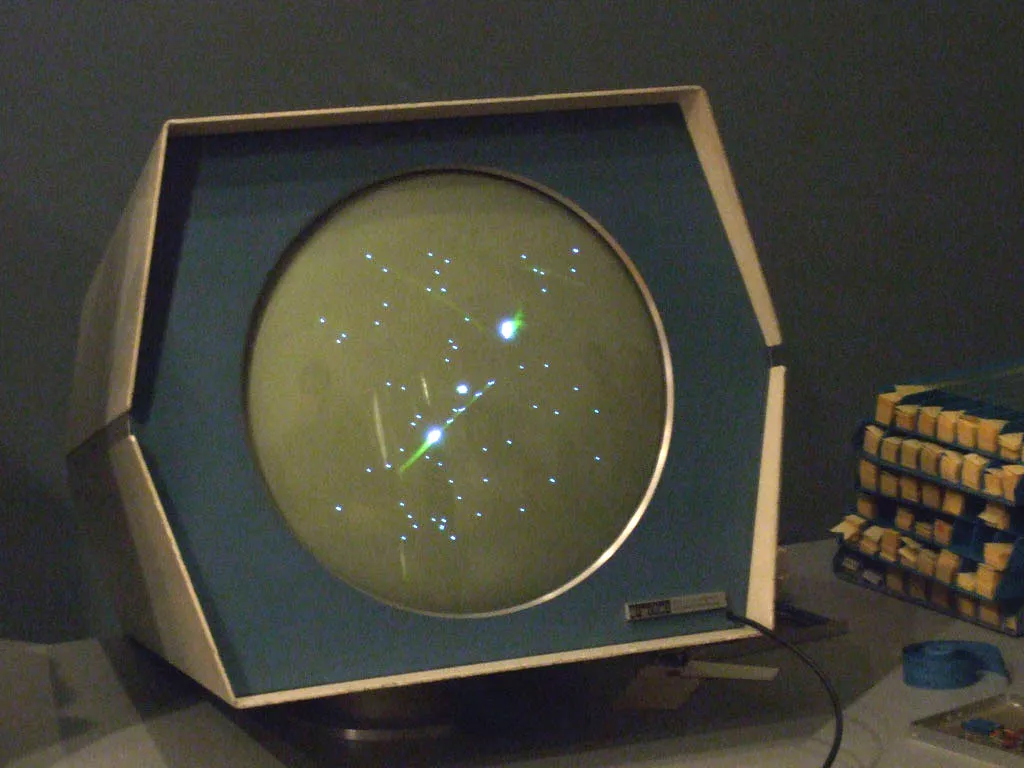
\includegraphics[width=0.53\textwidth]{obrazky-figures/ch2/Spacewar.png}
	\caption{Ukázka hry Spacewar.~\cite{bellis2019spacewar}}
	\label{fig:spacewar}
\end{figure}

%--------------------------
% Labyrintové hry
\section{Labyrintové videohry}
Dle Akademického slovníku současné češtiny~\cite{AkademickySlovnik-Bludiste} je bludiště, neboli labyrint, definováno jako \uv{místo, kde se bloudí} a \uv{složitý, neuspořádaný systém}. Bludiště jsou mnohocestné, je to tedy spleť cest, chodeb a prostor, kde se snadno zabloudí a jsou definovaná slepými konci a~větvícími se chodbami, kvůli kterým je procházející nucen se rozhodovat.

Andrew Rollings a Ernest Adams definují bludiště ve hrách jako prostředí, kde každé místo vypadá stejně, nebo velmi podobně a hráč musí zjistit, jak jsou místa propojená, často jejich procházením, aby našel cestu ven~\cite{rollings2003andrew}. Tyto hry jsou často doplněné i o nějaké jiné výzvy, než je pouze procházení bludištěm, kterými (dle stejných autorů~\cite{rollings2003andrew}) může být například hledání klíče k otevření zamknutých dveří, sbírání věcí (např. pro zvýšení skóre), řešení hádanek, paměťových testů, luštění kryptických zpráv, atd.

V 80. letech 20. století měly hry s tématem bludiště největší rozmach, hlavně díky rozšíření domácích konzolí (např. Atari 2600). Díky jejich množství a rozmanitosti je lze rozdělit na 4 typy~\cite{DoYouMaze}:
\begin{itemize}
    \item bludiště s pohledem z vrchu\,--\,při hraní je vidět celé (či skoro celé) bludiště z vrchu (Mouse in the Maze, Bomberman),
    \item bludiště s pohledem z první osoby\,--\,stejný pohled na hru, jako herní postavička (Maze/Maze War, Capture the Flag),
    \item pronásledování bludištěm\,--\,hráč je pronásledován, či může pronásledovat nepřátele; tento typ je propojen s různými styly pohledu na bludiště (Pac-Man, Rally-X, Lady Bug),
    \item bludiště s obsazováním políček mřížky\,--\,hráč při průchodu bludištěm musí zabrat co nejvíce políček (Amidar).
\end{itemize}

\noindent Dále v textu se nachází příklady různých významných labyrintových her vytvořených v~průběhu historie.

\begin{figure}[H]
	\centering
	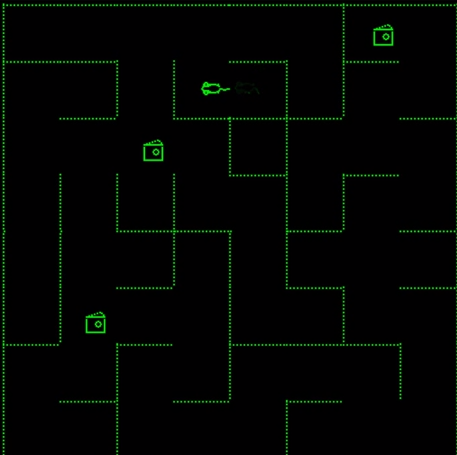
\includegraphics[width=0.5\textwidth]{obrazky-figures/ch2/MOUSE.png}
	\caption{Ukázka ze hry Mouse in the Maze.~\cite{Videogamehistorian}}
	\label{fig:mouse}
\end{figure}

\subsection*{Mouse in the Maze}
První labyrintovou videohrou byl titul s názvem \textit{MOUSE} neboli také \textit{Mouse in the Maze}, naprogramovaná roku 1959  Douglasem T. Rossem a John E. Wardem na sálovém počítači TX-0~\cite{TheOriginOfSpacewar}. 

Hráč dostal 8×8 mřížku a následně mohl světelným perem odmazat zdi a přidat sýr(y) (v upravené verzi martini) a následně sledovat myš procházející bludiště, kde si pamatovala již prošlé cesty, a hledající sýr, který musela najít, než se vyčerpala~\cite{Videogamehistorian}. Ukázka ze hry je zobrazena na obrázku~\ref{fig:mouse}, ze kterého je vidět, že hra je bludiště s pohledem z vrchu.

\subsection*{Maze/Maze War}
3D labyrintová pronásledující střílecí hra z roku 1974 vyvinutá studenty MIT~\cite{Maze_War}. Byla to průlomová hra, nabízející nejen iluzi 3D grafiky, ale i podporou hraní až pro 8 hráčů, či nehráčské boty. Byla nejspíše jednou z prvních, či možná i první střílecí hrou~\cite{virtual_worlds}. Později byla hra, díky využití TCP/IP protokolu, který hráčům umožnil hraní po internetu, průkopníkem i v online hrách~\cite{Maze_War}.

Úkolem hráčů, hrajících jako avatar oční bulvy, bylo projít bludiště (kde mohli chodit pouze dozadu, dopředu a otáčet se o 90° vpravo, či vlevo), najít nepřátele a střelit je, čímž sbírali skóre~\cite{Maze_War}.

\subsection*{Pac-Man}
Japonská arkádová hra od společnosti Namco (dnes Bandai Namco Entertainment) vyšla původně v roce 1980 pod jménem Puck-Man (kvůli jeho tvaru puku, jméno ale bylo pro USA změněno kvůli strachu z vandalů~\cite{kent2010ultimate}) a po svém vydání v USA se z ní stal okamžitý hit. V jediném roce se prodalo více než 100 000 arkádových automatů s touto hrou~\cite{PACMAN}. Hitem byly i další hry z rychle rostoucí série Pac-Man. Roku 1981 vyšla Ms. PAC-MAN, jež získala několik nových herních prvků, jako například více bludišť (oproti pouze jednomu, které nabízel originál), či náhodnější nepřátele\,--\,po svém vydání prodala i tato hra v USA více než 100 000 automatů, což žádná jiná hra v USA nedokázala~\cite{kent2010ultimate}.

\begin{figure}[hb]
	\centering
	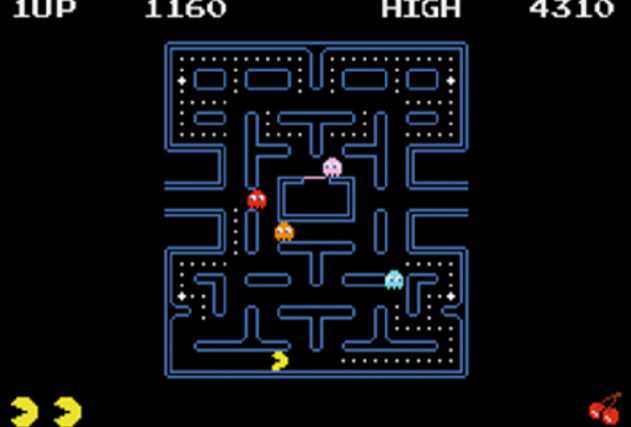
\includegraphics[width=0.7\textwidth]{obrazky-figures/ch2/pacman.png}
	\caption{Ukázka ze hry Pac-Man.~\cite{von2007space}}
	\label{fig:pacman}
\end{figure}

Pac-Man je hra založená na principu pronásledování hráče nepřáteli v bludišti~\cite{kent2010ultimate}, jak je vidět na obrázku~\ref{fig:pacman}. Hráč má za úkol projít bludiště a sebrat všechny tečky na zemi, čímž se dostane do další úrovně. Při tom ho ale pronásledují 4 duchové., Pokud ho chytí, tak Pac-Man ztratí jeden ze tří životů (když ztratí všechny, hra končí). Hráč dále může získat bonusové body díky sebranému ovoci, nebo pomocí bonusů, které mu umožní po omezenou dobu naopak duchy pojídat.

\subsection*{Bomberman/Dyna Blaster}
Další labyrintová hra od japonských vývojářů, která je podobně jako Pac-Man populární a~dodnes vydávaná, je Bomberman. V Evropě je též známý pod názvem Dyna Blaster. Vydán byl v roce 1983 (1985 na Nintendo konzole), kterého se prodalo za prvních několik let téměř milion kopií~\cite{Bomberman}. 
Mapa hry je jednoduchý obdélník s několika systematicky rozmístěnými nerozbitnými zdmi, mezi nimiž se nachází volná místa a rozbitné zdi. Hráčův úkol je porazit všechny nepřátele v lokaci pomocí pokládání bomb, které po určitém čase vybuchnou v~křížovém tvaru, čímž zlikvidují nepřátele a rozbijí zdi v jeho výbušné oblasti~\cite{Bomberman}. 

%--------------------------
% Herní engine
\section{Herní engine}\label{chap:Herní engine}
Herní engine (také game engine) je softwarový framework využívaný pro tvorbu a vývoj (nejen) videoher. Nabízí mnoho nástrojů pro zjednodušení tvůrčího procesu, jako jsou například podpůrné programy a knihovny. Některé poskytují také speciální programovací jazyky vytvořené specificky pro programovaní her v daném enginu~\cite{Valencia-Garcia_2016}. V následující části textu jsou uvedeny a popsány některé příklady z nejpopulárnějších herních enginů (viz obrázek~\ref{fig:most_popular_game_engines}).
\begin{figure}[H]
    \vspace{1cm}
	\centering
	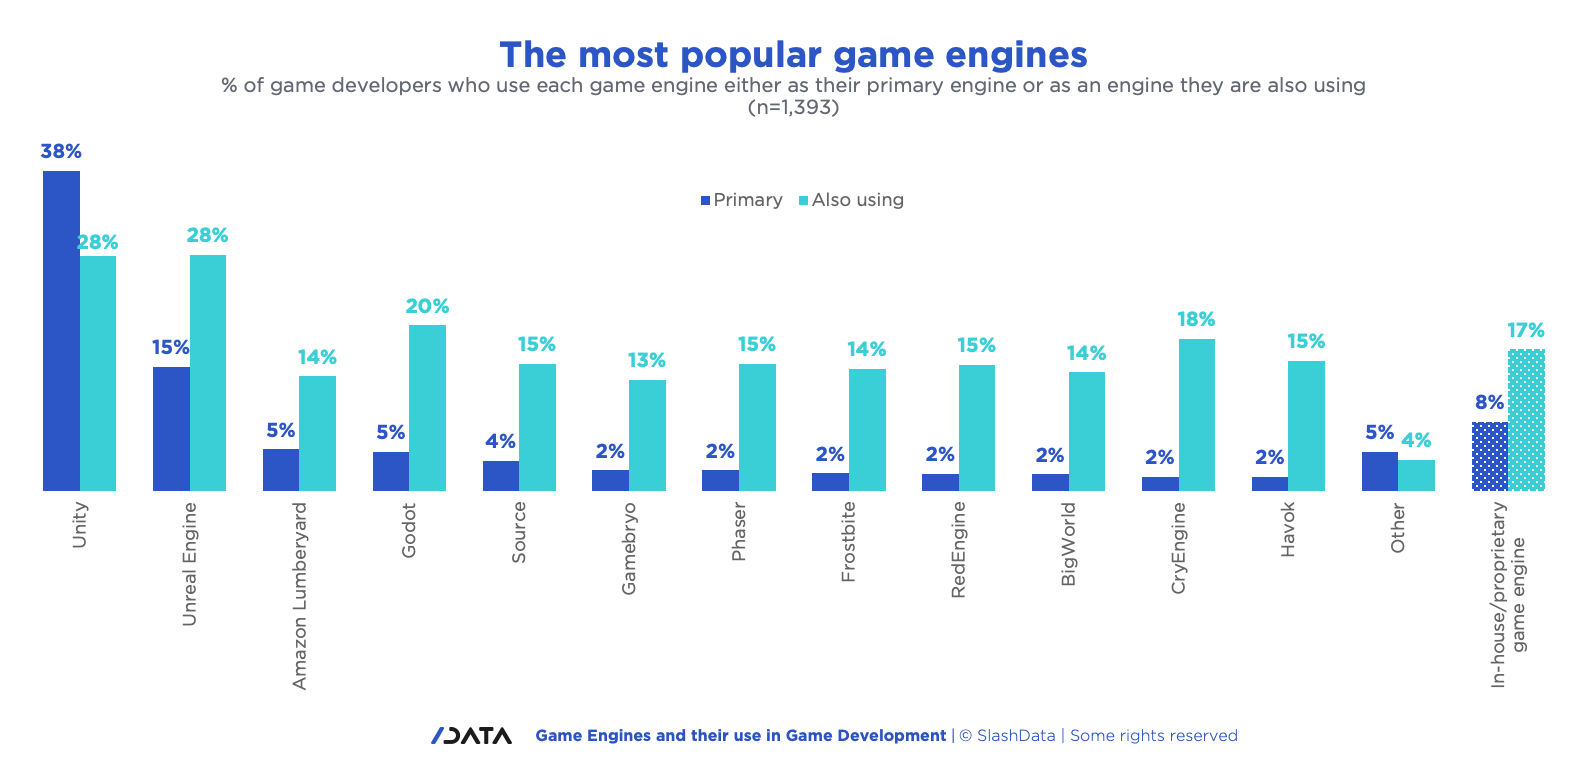
\includegraphics[width=\textwidth]{obrazky-figures/ch2/most_popular_game_engines.png}
	\caption{Výzkum SlashData z roku 2021 o nejpoužívanějších herních enginech.~\cite{SlashData_game-engines}}
	\label{fig:most_popular_game_engines}
\end{figure}

\subsection*{Unity}
Unity je multiplatformní game engine od společnosti Unity Technologies. Dle oficiálních webových stránek aktuálně podporuje více než 20 platforem (např. Windows, macOS, Linux, Android, PlayStation 5, Nintendo Switch,~\ldots)~\cite{unity_website}, nejen díky čemuž je jedním z~nejpoužívanějších enginů pro tvorbu her~\cite{arnia_unity}. Poskytuje bezplatnou verzi (pro soukromé užití, nebo pokud výdělek hry za rok nepřesahuje 100 000\$) i placenou verzi \uv{Unity Pro}. 

Pro implementaci her, ať už 2D, 3D či VR (hry pro virtuální realitu), nabízí možnost vizuálního/grafického editoru a skriptů v C\#. Základní herní entita je \verb|GameObject|, které je možné přiřazovat různé vlastnosti, herní mechaniky, grafiku atd. Ty mohou být předefinované, či naprogramované uživatelem pomocí skriptů. Různé \verb|GameObjects| můžou být součástí \verb|Scene| z čehož je následně konstruován finální produkt~\cite{hocking2015unity}.

Unity je hojně využíváno na vývoj AAA (také Triple-A hry neboli produkt od distributora, pro jehož vývoj byl k dispozici bohatý rozpočet) her, například: Marvel Snap, Apex Legends, ale i indie her (takzvaně od nezávislých tvůrců = independent creator), například: Cult of the Lamb, Among Us, Slime Rancher, Cuphead~\cite{unity_website}.

\subsection*{Unreal Engine}
Unreal Engine je série herních enginů s nejnovější verzí Unreal Engine 5 z roku 2022 od společnosti Epic Games. Poprvé byl představen ve hře Unreal, 3D střílečce z pohledu první osoby. Ta byla velmi populární, jelikož díky UnrealScriptu (založeném na C++) mohli uživatele jednoduše původní hru modifikovat~\cite{sanders2016introduction}. Novější verze využívají klasické C++. Podobně jako Unity nabízí bezplatnou i placenou verzi. Je také multiplatformní, ale podporuje menší škálu platforem než Unity\,--\,např. Windows, Linux, PlayStation, Nintendo Switch, Xbox~\cite{unreal_engine}.

V porovnání s dalšími zástupci herních enginů je hodnocen jako jeden ze složitějších. Díky své komplikovanější stavbě a strmé křivce učení je doporučován spíše na větší, komplikovanější projekty, než například na mobilní hry (i přestože podporuje vývoj her na Android)~\cite{Kevuru_Games_Unreal-Unity}. Unreal Engine 5 je zaměřený primárně na 3D vývoj a proto přišel s~mnoha funkcemi pro vylepšení vykreslování a práci s třídimenzionálními objekty - jsou to Nanite (vizuální geometrický systém), Lumen (vylepšená práce se světlem) a MetaSounds (managment audia)~\cite{UnrealEngine5}.

Hrami, které byly vytvořeny za pomocí Unreal Enginu, jsou například Minecraft Dungeons, Final Fantasy VII Remake, Fortnite (ukázka na obrázku~\ref{fig:fortnite-unreal_engine}) nebo Stray~\cite{unreal_engine}.

\begin{figure}[H]
	\centering
	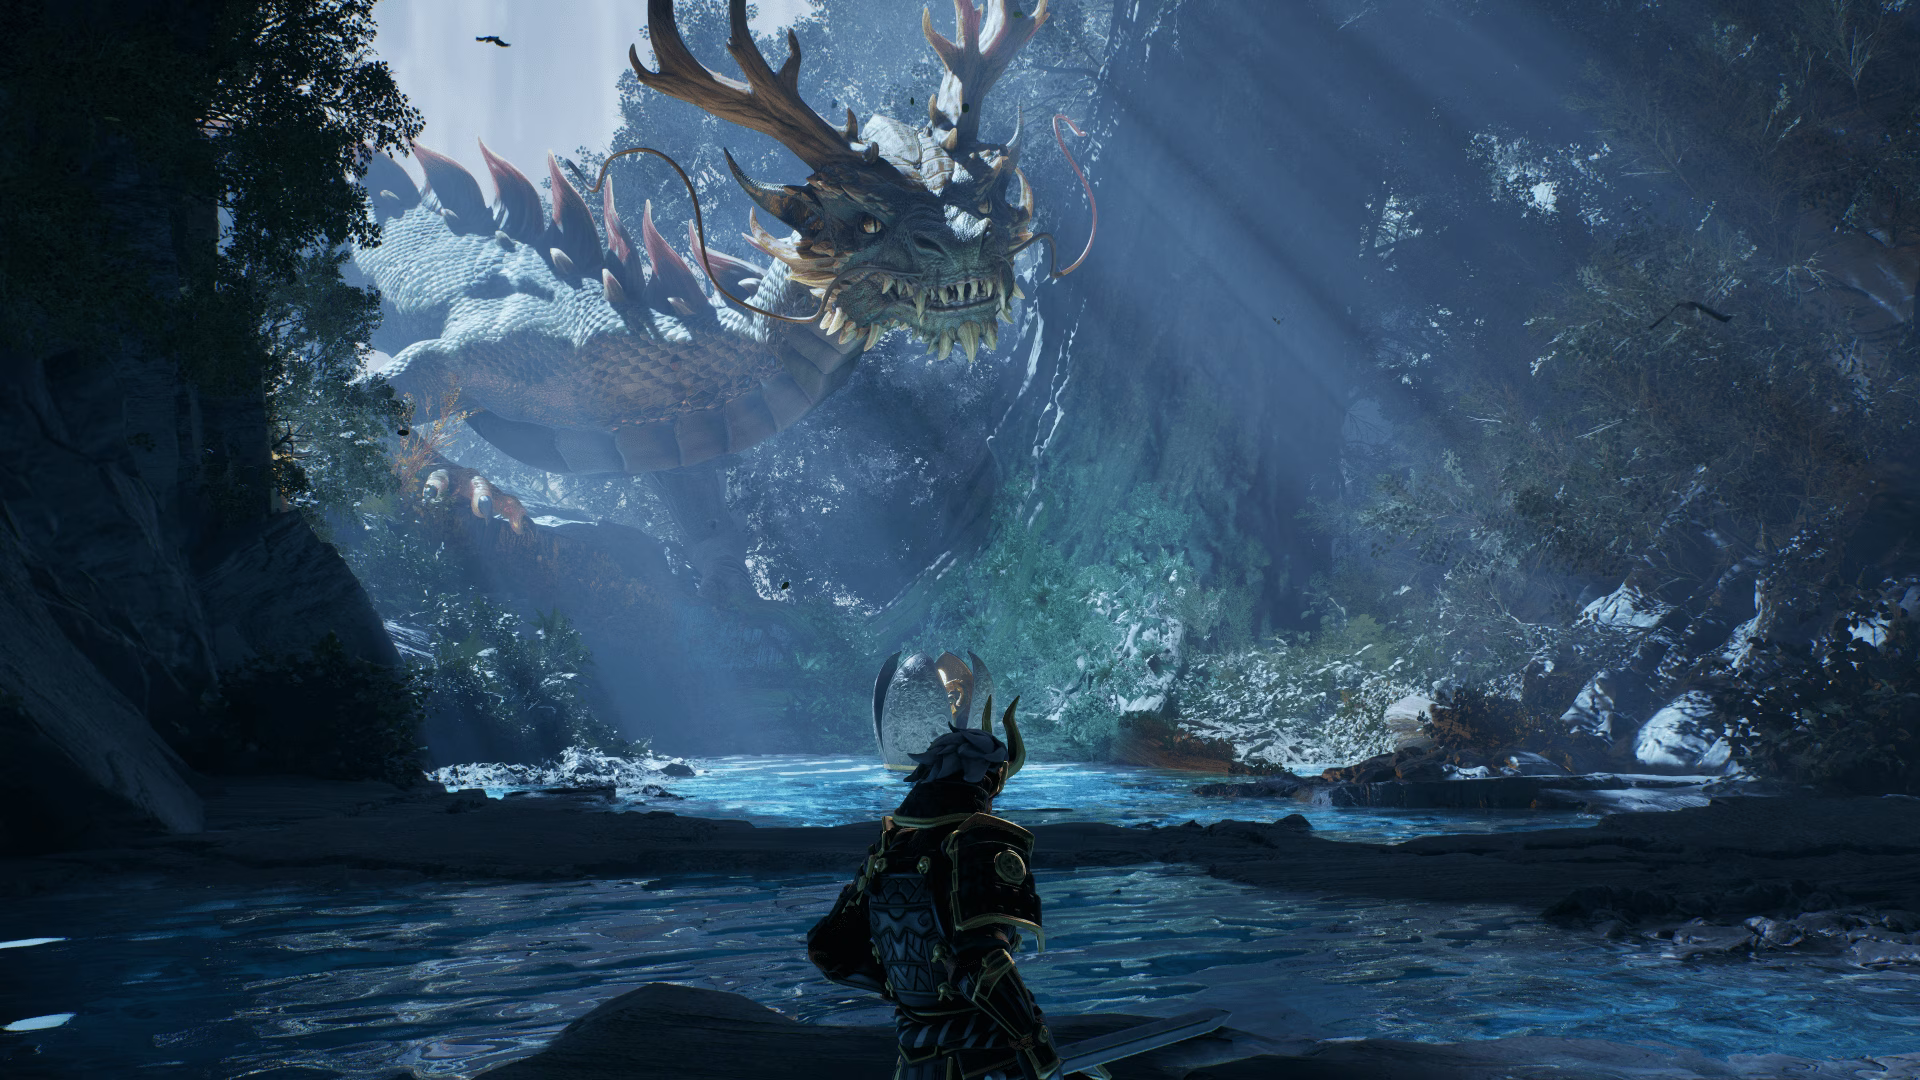
\includegraphics[width=0.66\textwidth]{obrazky-figures/ch2/fortnite.png}
	\caption{Ukázka ze hry Fortnite vytvořená pomocí Unreal Engine 5.~\cite{unreal_engine}}
	\label{fig:fortnite-unreal_engine}
\end{figure}

\subsection*{Godot}
Godot (s aktuální verzí Godot 4) je další software pro tvorbu 3D a 2D her. Na rozdíl od Unity a Unreal Enginu je od verze 3.0 kompletně zdarma, svobodný a otevřený (open-source)\footnote{\url{https://github.com/godotengine/godot}}. Z toho důvodu má Godot ve srovnání s jinými zmíněnými herními enginy omezené oficiální možnosti platforem, jelikož jsou konzole (PlayStation, Xbox, Nintendo) uzavřené ekosystémy a Godot nimi není licencovaný~\cite{Godot_Engine_consoles}. Stále ale podporuje škálu platforem, jako jsou desktopové (Windows, Linux, macOS), webové (HTML5), mobilní (Android, iOS) a~virtuální realita (Oculus Rift/Quest, HTC Vive).

Základní stavební blok pro vytváření projektu v Godotu je \verb|Node| (objekt reprezentující specializovaný prvek)\,--\,tyto objekty lze následně propojovat do \verb|Scene|, jak je vidět na obrázku~\ref{fig:godot_view}, což jsou stromy závislostí tvořící finální produkt~\cite{bradfield2018godot}. K těmto \verb|Nodes| lze přiřazovat skripty v jazycích GDScript (dynamicky typovaný jazyk syntaxí podobný Pythonu), C\# a C++\cite{GameEngineWizardry}. Godot se oproti předešlým zmíněným softwarům zaměřuje na 2D, pro které nabízí optimalizovaný přístup zdůrazňující jednoduchost a efektivitu (např. \verb|TileMap|, pro tvoření map, či \verb|Sprite2D| s vlastnostmi pro funkci 2D postav)~\cite{Godot_Engine}.

V Godotu byly vytvořeny například hry Brotato, Hive Time, Tail Quest a aplikace Dungeoncraft a Material Maker~\cite{Godot_Engine}.
\begin{figure}[H]
	\centering
	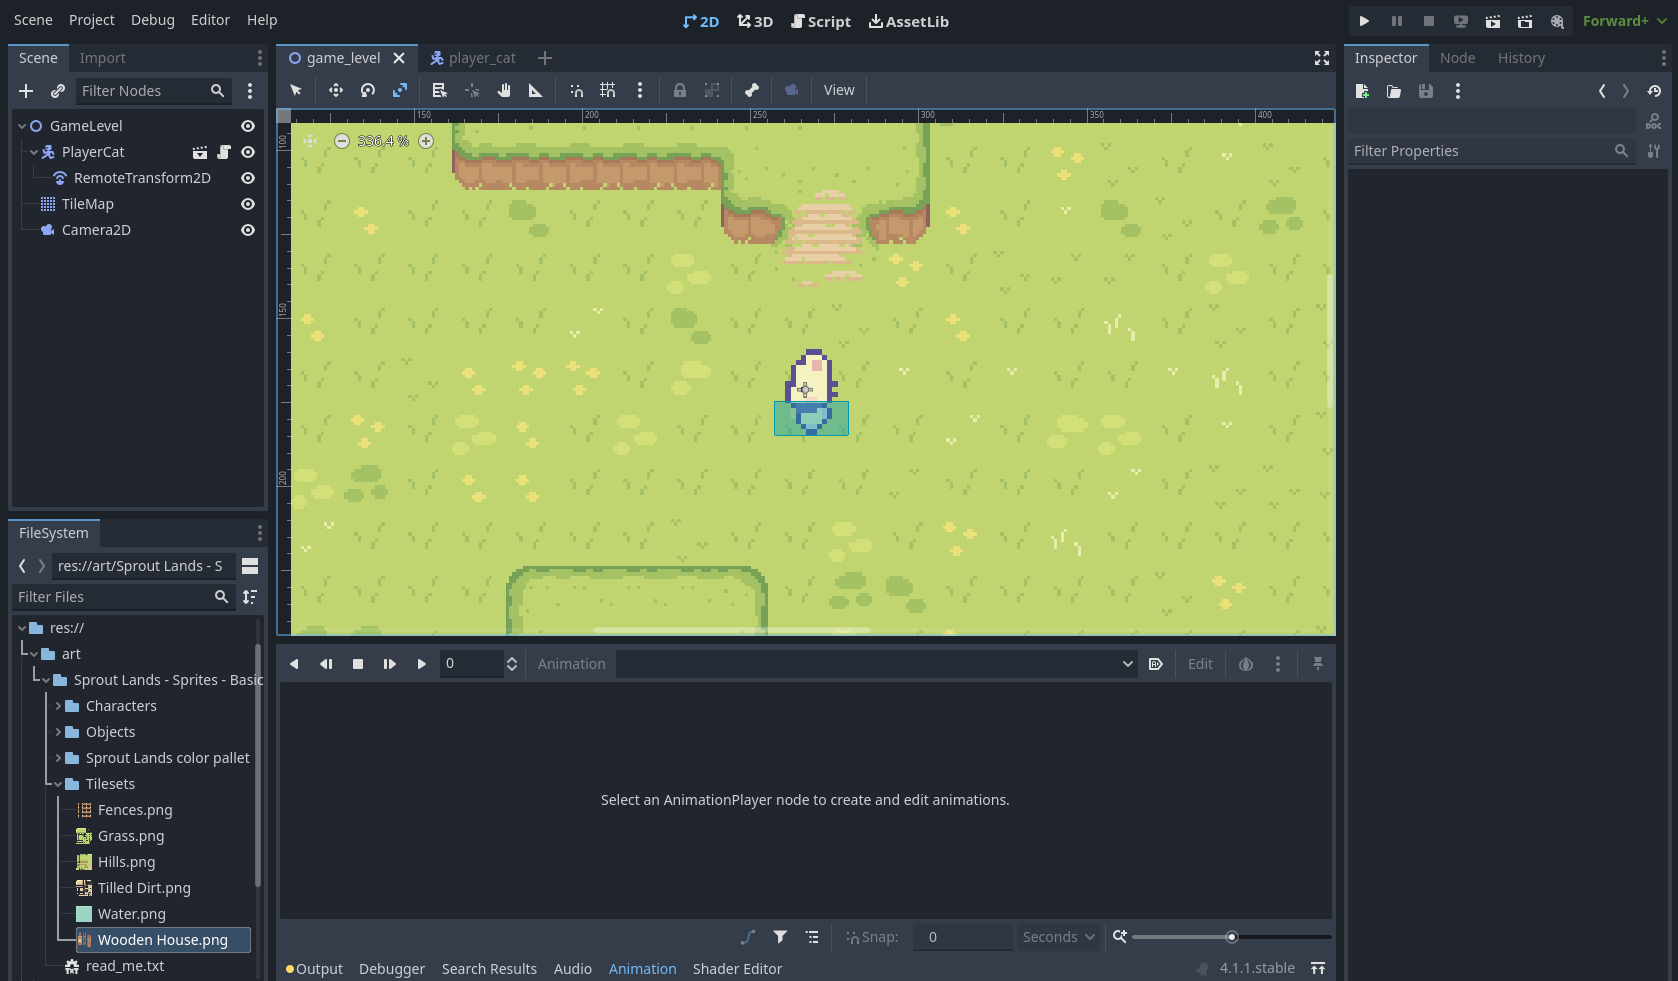
\includegraphics[width=0.8\textwidth]{obrazky-figures/ch2/godot_view.png}
	\caption{Grafické rozhraní pro zobrazení Scene v Godotu 4.}
	\label{fig:godot_view}
\end{figure}

%--------------------------
% Celulární automaty
\section{Celulární automaty}\label{chap:Celulární automaty}
Celulární automat (dále označován také zkratkou CA) je dynamický systém a diskrétní model prostorového systému využívaný na modelování fyzikálních či biologických simulací. Prostorový systém vyjadřuje prostorovou dekompozici systému\,--\,zkoumaný systém je rozdělen na malé části s definovaným chováním~\cite{ims}.

\subsection*{Základní definice }
Celulární automat je čtveřice ${(\alpha^{n}, S, N, f)}$, kterou lze dle Stanfordské encyklopedie filozofie~\cite{sep-cellular-automata}, definovat následovně:
\begin{itemize}
    \item ${ \alpha^{n} }$ (\textit{Lattice}) je diskrétní n-dimenzionální mřížka buněk (${ n >= 1 }$)\,--\,tyto buňky jsou identické (některé mohou být speciální\,--\,např. modelují pevné hranice), 
    \item ${ S }$ je konečná množina stavů, kterých mohou buňky nabývat\,--\,v každém diskrétním časovém kroku může každá buňka nabývat pouze a jenom 1 stavu, 
    \item ${ N }$ je konečná množina sousedících buněk (okolí, které může, či nemusí obsahovat i~buňku samotnou) pro každou buňku, na kterém záleží její vývoj, ${ N \subseteq \alpha }$,
    \item ${ f }$ je konečná množina pravidel pro přechod mezi stavy\,--\,v každém časovém kroku každá buňka aktualizuje svůj aktuální stav podle deterministické přechodové funkce $\phi : \Sigma^n \rightarrow \Sigma$, která mapuje okolí. Často (i když ne nutně) se počítá, že aktualizace je synchronní a v čase $t$ bere jako vstup stav svého okolí v bezprostředně předchozím časovém kroku $t-1$.
\end{itemize}
Příkladem definice celulárního automatu Game of Life (vysvětlený níže) je následující zápis:
\begin{equation*}
\begin{split}
    & \left( \alpha^{2}, \right. \\
    & \left. \{0, 1\}, \right. \\
    & \left. N(c_i) = \{ c_{i-1,j-1}, c_{i-1,j}, c_{i-1,j+1}, c_{i,j-1}, c_{i,j}, c_{i,j+1}, c_{i+1,j-1}, c_{i+1,j}, c_{i+1,j+1} \}, \right. \\
    & \left. \{B3/S23\} \right)
\end{split}
\end{equation*}

Vlastnosti CA je možné popsat také pomocí řetězců pravidel (anglicky \textit{rulestring}). V~následujícím textu jsou uvedeny 2 příklady přebrané ze stránky LifeWiki~\cite{LifeWiki} pro 2 stavové CA. Těmito stavy jsou 1 = živá buňka a 0 = mrtvá buňka. 
\begin{itemize}
    \item Birth/Survival notace\,--\,Nejpoužívanější notace, která je zapisována pomocí \verb|B{list}| \verb|/S{list}|. Notace je vyjadřována dvěma seznamy. V prvním (B) je zapsán počet živých sousedů potřebný pro vznik nové živé buňky, neboli oživení. Druhý seznam určuje kolik živých sousedů musí buňka mít, aby přežila do dalšího kroku. Game of Life by touto notací byla zapsána jako B3/S23.
    \item S/B notace\,--\,Dříve často používaná, dnes spíše nahrazena Birth/Survival notací. Podobně jako ona je zapisována pomocí dvou seznamů \verb|{list}|\verb|/{list}|. Jeden označuje počet živých sousedů potřebných pro přežití živé buňky a druhý počet živých sousedů potřebných pro oživení mrtvé buňky. Tedy opak Birth/Survival listu. Game of Life je zapsána jako 23/3.
\end{itemize}

Typ okolí závisí na tvaru buněk (čtverec, hexagon,~\ldots) a také typu prostoru (1D, 2D,~\ldots)~\cite{ims}. Dvě nejpoužívanější okolí jsou Moorovo a von Neumannovo s různými variacemi~\cite{sloot2004cellular}, jak je vidět na obrázku~\ref{fig:2D-okoli}.
\begin{figure}[H]
    \centering
    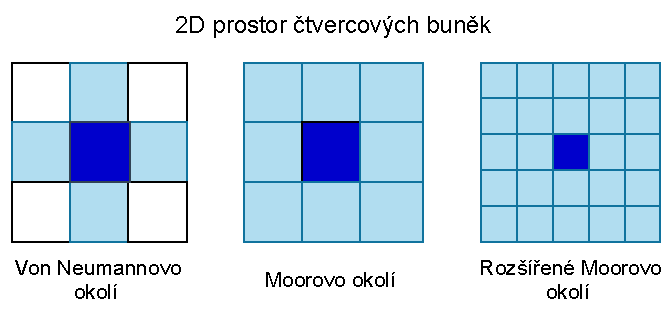
\includegraphics[width=0.65\textwidth]{obrazky-figures/ch2/2D-okoli.pdf}\hspace{0.5cm}
    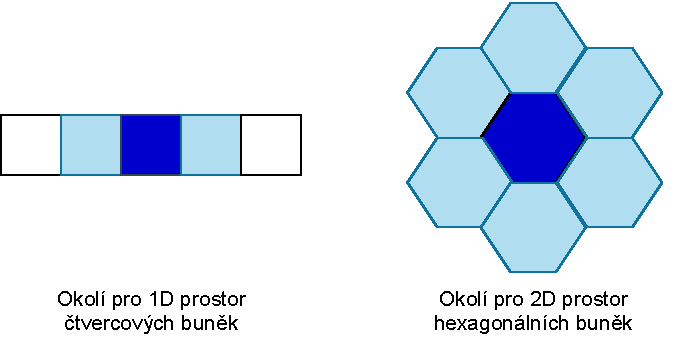
\includegraphics[width=0.65\textwidth]{obrazky-figures/ch2/jina-okoli.pdf}
    \caption{Příklady okolí (tmavě modrá = zkoumaná buňka, světle modrá = okolí).}
    \label{fig:2D-okoli}
\end{figure}

Jak je již popsáno u formálního popisu, pravidla určují následující stav buňky v čase, který je závislý pouze na jejím aktuálním stavu a stavu jejího okolí, a to pro všechny možnosti vstupu. Pomocí funkce stavu buňky ${s(t)}$ a jejího okolí ${N_s(t)}$ lze vyjádřit rovnici~\ref{eq:CA-rule} pravidla~\cite{ims}.
\begin{equation}
s(t + 1) = f(s(t), N_s(t))
\label{eq:CA-rule}
\end{equation}
Některá pravidla mohou mít i vlastnosti udávající typ pravidla, které definuje~\cite{mechanics-CA}:
\begin{itemize}
    \item \textbf{totalistic} = o výsledku rozhoduje součet hodnot vstupních buněk (např. Game of Life),
    \item \textbf{legal} = z nulového vstupu nemůže samostatně vzniknout nenulový.
\end{itemize}

\subsection*{Klasifikace}
Stephen Wolfram ve své knize \textit{A New Kind of Science}~\cite{wolfram-NewKindOfScience} definoval 4 třídy pro dělení CA, vypsané níže.
\begin{enumerate}
    \item Téměř všechny počáteční vzory CA se po konečném počtu kroků dostanou do jednoho stabilního, homogenního stavu. Zmizí jakákoliv náhodnost v počátečním vzoru.
    \item Téměř všechny počáteční vzory CA se vyvinou do periodicky se opakujících (oscilujících) struktur/stavů nebo zůstane stabilně v některém ze stavů.
    \item Deterministický chaos\,--\,téměř všechny počáteční vzory se vyvíjejí pseudonáhodným, nebo chaotických způsobem. Stabilní struktury, které se objeví, jsou rychle zničeny okolním šumem.
    \item Téměř všechny počáteční vzory se vyvíjejí do struktur, které interagují složitým a~zajímavým způsobem s tvorbou místních struktur, které jsou schopny přežít po dlouhou dobu. Konečným výsledkem mohou být stabilní nebo oscilující struktury typu 2 (k~dosažení může být ale potřeba velký počet kroků). Pod tuto třídu patří Game of Life (viz níže).
\end{enumerate}

Některé celulární automaty lze označovat také jako \textbf{reverzibilní}. Ty jsou definované jako systémy, které neztrácí informaci při svém vývoji v čase\,--\,což znamená, že v každém okamžiku lze otočit vývoj času a navrátit se k předchozím stavům~\cite{ims}. Kvůli jejích chaotickému chování nejsou CA 4. třídy nikdy reverzibilní.

\subsection*{Historie a Game of Life}
Za vznikem celulárních automatů stáli ve 40. letech 20. století matematici John von Neumann a~Stanisław Ulam. Ulam studoval růst krystalů pomocí jednoduché mřížky~\cite{pickover2009math} a~von Neumann řešil modely samoreprodukujících se organismů~\cite{history_CA}. Ulam navrhl von Neumannovi využití diskrétního systému~\cite{schiff2011cellular} s buňkami, které se mění po jednotlivých krocích/iteracích. Na základě dalšího výzkumu došli k vyvinutí základů CA a John von Neumann následně na základě myšlenek celulárních automatů sepsal knihu \textit{Theory of Self-Reproducing Automata}, kde detailně, spolu s důkazy o jeho možné existenci, popisuje jeden z prvních konceptů realistického samo-replikujícího systému, \textit{von Neumannův univerzální konstruktor}~\cite{theory_neumann} který funguje jako univerzální kopírka, jež by v teorii replikovala sebe sama pomocí surovin z prostředí, ve kterém se nachází. 

Dalším z důležitých matematiků pro vývoj CA byl John Conway, který v roce 1970 vytvořil pravidla pro \textbf{Game of Life}~\cite{history_CA}, celulární automat na 2D mřížce s buňkami nabývajících 2 stavů\,--\,živá, mrtvá, využívající Moorovo okolí o 8 sousedech (viz obrázek~\ref{fig:2D-okoli}). Pravidly jsou~\cite{Game_Of_Life}:
\begin{itemize}
    \item pokud živá buňka sousedí s 2 nebo 3 živými sousedy přežívá do další generace,
    \item neživá buňka, která má přesně 3 živé sousedy oživne,
    \item zbytek buněk do další generace nepřežívá a stává se mrtvými.
\end{itemize}
I přes svoji jednoduchost tento systém nabývá klasifikace 4. třídy, tedy projevuje náhodnost, ale zároveň se v jeho generacích objevují struktury, které vykazují rozmanité vlastnosti a~dodávající systému částečný řád. Jednou z těchto struktur, je takzvaný kluzák (anglicky \textit{glider}), který se postupem iterací pohybuje po mřížce~\cite{Game_Of_Life}. Ilustraci jeho pohybu je možné vidět na obrázku~\ref{fig:game_of_life}.
\begin{figure}[H]
    \centering
    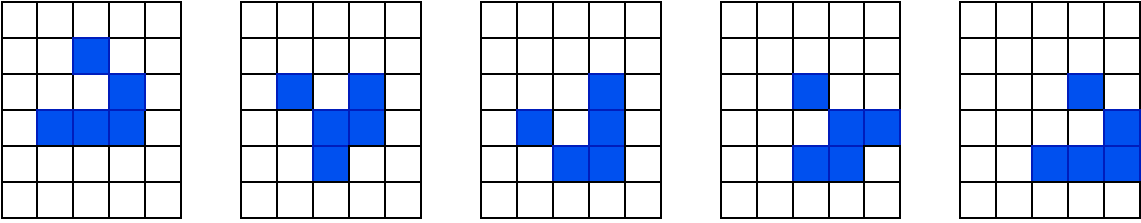
\includegraphics[width=\textwidth]{obrazky-figures/ch2/GameOfLife.pdf}
    \caption{Pohyb kluzáku/glideru v CA Game of Life.}
    \label{fig:game_of_life}
\end{figure}

\begin{figure}[H]
    \centering
    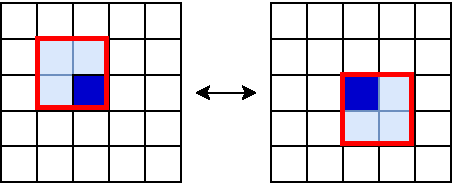
\includegraphics[width=0.65\textwidth]{obrazky-figures/ch2/Margolus.pdf}
    \caption{Margolusovo okolí (tmavě modrá = zkoumaná buňka, červená = 2×2 blok, světle modrá = okolí).}
    \label{fig:Margolus}
\end{figure}

Posledním, zde zmíněným, důležitým vědcem v historii CA byl Stephen Wolfram, který, jak již bylo zmíněno, ve své knize \textit{A New Kind of Science}~\cite{wolfram-NewKindOfScience} popsal 4 třídy pro klasifikování celulárních automatů, a to podle jejich vztahu k druhému na základě fyzikálního zákonu zachování hmotnosti.

\subsection*{Využití celulárních automatů ve hrách}
Jedno z využití CA obsahují hry \uv{padajícího písku}, neboli \textit{Falling-sand games/simulators}. Tyto hry jsou nejčastěji 2D, sandboxové (= podporující kreativitu). Ty mohou být založeny například na blokových/rozdělujících celulárních automatech, které mohou simulovat reálnou fyziku, jelikož jsou reverzibilní a dodržují fyzikální zákon zachování~\cite{schiff2011cellular}. Nejjednodušší okolí využívané na vyhodnocení těchto CA je Margolusovo (viz obrázek~\ref{fig:Margolus})\,--\,2D mřížka je rozdělena na 2×2 čtverce, které se každou generaci posouvají diagonálně o~jednu buňku~\cite{schiff2011cellular} (okolí v čase t se tedy skládá ze všech buněk, které se nacházejí v bloku v aktuálním čase).

\noindent Hráč má při hraní hry přístup k několika materiálům/elementům, které mají každý své vlastní vlastnosti (gravitace, reaktivnost s jinými materiály).  S nimi může interagovat na dané ploše. Příkladem těchto her může být The Powder Toy\footnote{https://powdertoy.co.uk}, The Sandbox (2012), Sandspiel (ukázka na obrázku~\ref{fig:Sandspiel}) či Noita (hra doplněná o roguelike aspekty).
\begin{figure}[H]
    \centering
    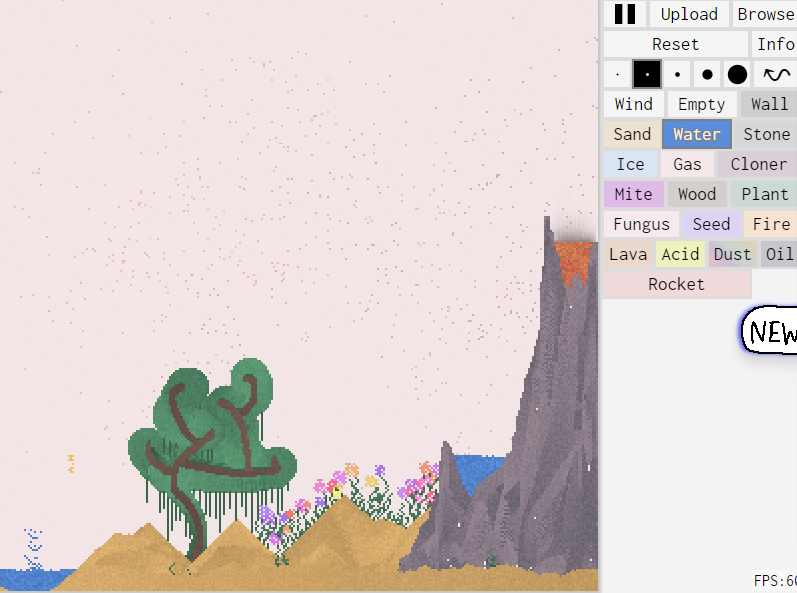
\includegraphics[width=0.55\textwidth]{obrazky-figures/ch2/SandSpiel.png}
    \caption{Ukázka ze hry Sandspiel.}
    \label{fig:Sandspiel}
\end{figure}

\begin{figure}[H]
    \centering
    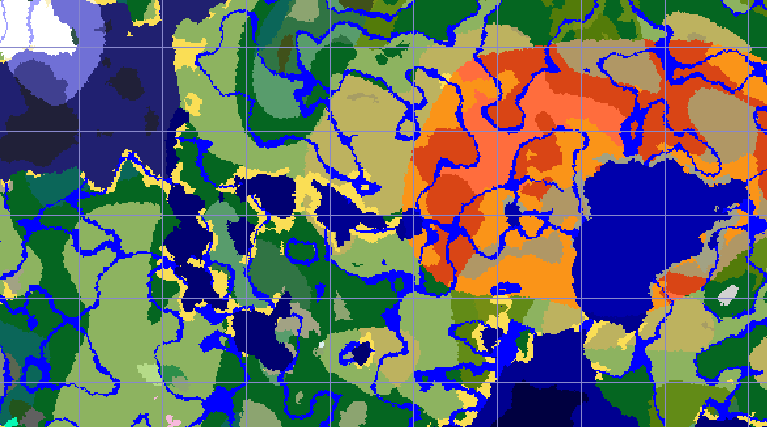
\includegraphics[width=0.7\textwidth]{obrazky-figures/ch2/minecraft_biom.png}
    \caption{Příklad vygenerovaného Minecaft světa s různými biomy.}
    \label{fig:minecraft_biom}
\end{figure}

Rozšířenější a v moderních hrách i častější, je využití CA na procedurální generování terénu. CA je využito hlavně u her vyžadujících větší a pestrý svět\,--\,například Minecraft, či vysoký počet úrovní vyžadujících rozmanité překážky. Důvodem je, že tradiční \uv{lidské} vytváření map může být nákladné kvůli několika příčinám. Manuální navrhovaní obrovské mapy, či 100+ úrovní lidmi zabere mnoho času, energie a může se objevit repetitivita vytvořeného prostředí. Tyto před-vytvořené mapy také zabírají mnoho paměti a jejich načítání může být obtížné na procesor\,--\,procedurální generace vytváří mapy za chodu aplikace, takže vyřeší oba problémy~\cite{Procedural_Game_Map}.

Minecraft například generuje základ své mapy díky stochastickým celulárním automatům spuštěným nad zpracovanými (např. pomocí šumu) výsledky kongruentních generátorů~\cite{Minecraft}. U stochastických/náhodných celulárních automatů nejsou pravidla deterministická (tj. předvídatelná), ale pravděpodobnostní. To znamená, že místo pevného pravidla určujícího následující stav buňky má zadané pravděpodobnosti možných nových stavů buňky~\cite{DBLP:journals/corr/abs-1304-7185}. Díky tomu dochází k definování přechodů a prolínání mezi různými poddruhy biomů (příklad vygenerované mapy je vidět na obrázku~\ref{fig:minecraft_biom}). Například teplé oblasti mají 50\% šanci, že se promění v poušť, 33\% v savanu a 17\% v roviny, nebo oceány mají 50\% šanci, že se promění v zem~\cite{Minecraft}.

Některé z jednodušších možností generování prostředí s celulárními automaty je využití algoritmů na náhodné generování jeskyní. Příkladem může být například algoritmus (zapsán níže algoritmem \ref{algo:cave_gen}) z naučné stránky envatotuts+~\cite{CaveCA}, kde každá buňka CA může nabývat 2 stavů\,--\,živá, mrtvá. Výsledek tohoto algoritmu je na obrázku~\ref{fig:cave}.
\begin{algorithm}
\caption{Generování jeskyní pomocí CA}\label{algo:cave_gen}
\begin{algorithmic}[1]
\State \textbf{Input:} $\text{matrix}, \text{row}, \text{col}, \text{deathLimit}, \text{birthLimit}$
\State \textbf{Output:} updated state of the cell
\State $\text{neighbors} \gets \text{countAliveNeighbours}(\text{matrix}, \text{row}, \text{col})$
\State $\text{cellValue} \gets \text{matrix[row, col]}$
\If{$\text{cellValue} = \text{alive}$}
    \If{$\text{neighbors} < \text{deathLimit}$} \Comment{Moc sousedů $\Rightarrow$ smrt} 
        \State \textbf{return} $\text{dead}$
    \Else \Comment{Přežití} 
        \State \textbf{return} $\text{alive}$
    \EndIf
\Else
    \If{$\text{neighbors} > \text{birthLimit}$} \Comment{Oživení} 
        \State \textbf{return} $\text{alive}$
    \Else
        \State \textbf{return} $\text{dead}$
    \EndIf
\EndIf
\end{algorithmic}
\end{algorithm}
\newline
Algoritmus funguje na několika jednoduchých principech, s nimiž je možné různě manipulovat, a to změnou hodnot \verb|deathLimit| a \verb|birthLimit|:
\begin{itemize}
    \item narození = pokud je buňka mrtvá a má určitý počet živých sousedů, v následující iteraci se oživí (podpora růstu jeskynních chodeb),
    \item smrt = pokud je buňka živá a má příliš málo mrtvých sousedů, zemře v následující iteraci (vytváření otevřených prostorů v jeskyni),
    \item přežití = pokud je buňka živá a má dostatečný počet živých sousedů, přežívá do následující iterace (udržování existující struktury jeskyní).
\end{itemize}

\begin{figure}[H]
\vspace{0.5cm}
    \centering
    
\includegraphics[width=0.6\textwidth]{obrazky-figures/ch2/cave.png}
    \caption{Příklad algoritmu generování jeskyní s využitím Moorova okolí,	deathLimit = 3, birthLimit = 4.}
    \label{fig:cave}
\end{figure}
\vspace{0.5cm}

Také je možné využít algoritmy generující strukturu podobnou bludišti. Celulárním automatem s touto vlastností je OCA:Maze~\cite{OCA:Maze}. Hlavním principem tohoto algoritmu s~Mooreovým okolím je, že pokud má buňka živých 1 až 5 sousedů, tak přežije a ožívá pokud má přesně 3 sousedy. To znamená, že je pro buňky složitější zemřít a tím se vytváří vzory podobné bludišti, jak je vidět v levé částí obrázku~\ref{fig:OCA:Maze}. Při generování s náhodnou matici, ale nejsou cesty zcela propojené, získáváme jen mnoho nepropojených místností. Existuje i~jeho upravená verze (Mazectric), která omezuje počet sousedů potřebný přežití na 1~až~4, díky čemuž vznikají rovnější a delší \uv{cesty}~\cite{OCA:Maze}, což je možné vidět na pravé částí obrázku~\ref{fig:OCA:Maze}.
\begin{figure}[H]
    \centering
    
\includegraphics[width=0.47\textwidth]{obrazky-figures/ch2/OCA:Maze.png}\hspace{0.5cm}
    
\includegraphics[width=0.47\textwidth]{obrazky-figures/ch2/Mazectric.png}
    \caption{Porovnání výsledků CA OCA:Maze (vlevo) a Mazectric (vpravo).}
    \label{fig:OCA:Maze}
\end{figure}
    
%--------------------------
% Prohledávání stavového prostoru
\section{Prohledávání stavového prostoru}
Stavový prostor (anglicky \textit{State space}), využívaný na řešení úloh, lze v informatice popsat jako orientovaný graf, v němž jeho uzly reprezentují stavy a hrany reprezentují operátory, či stavové přechody~\cite{State-Space_Search}. Formálně je možné stavový prostor a jeho aktuální řešenou úlohu zapsat jako čtveřici (S, O, $s_0$, G), jejíž prvky lze definovat následovně~\cite{izu}:
\begin{itemize}
    \item S je množina všech možných stavů,
    \item O je množina všech přechodů mezi stavy/operátorů, kterými lze měnit stavy,
    \item $s_0$ je počáteční stav řešené úlohy, $s_0 \in S$,
    \item G je neprázdná podmnožina S cílových stavů úlohy.
\end{itemize}
Úlohy lze řešit buď díky neinformovaným/slepým metodám, nebo informovaným metodám, které jsou popsány níže. 

\subsection*{Neinformované metody}
Nazývají se neinformovanými neboli slepými, jelikož nemají žádné začáteční informace o~prostoru a umístění cíle. Což znamená, že tyto vyhledávající metody systematicky prohledávají stavový prostor a dokud nenajdou zadaný hledaný výsledek, tak pouze pokračují v \uv{prolézání} prostorem~\cite{poole2023artificial} (či neúspěšně prohledají všechny části stavového prostoru). Dále v~kapitole jsou popsány některé příklady metod tohoto typu.

\subsubsection*{\textbullet Metoda slepého prohledávání do šířky (BFS)}
Metoda funguje na principu fronty FIFO (\textit{= first-in, first-out}), do níž postupně zapisuje uzly, které jsou objeveny, ale neprohledány~\cite{poole2023artificial}. 

\begin{figure}[H]
    \centering
    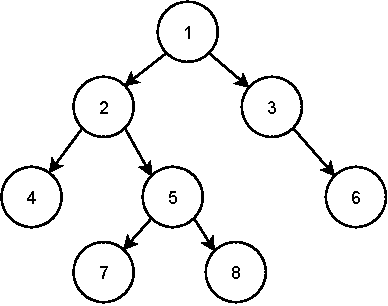
\includegraphics[width=0.48\textwidth]{obrazky-figures/ch2/BFS.pdf}\hspace{0.25cm}
    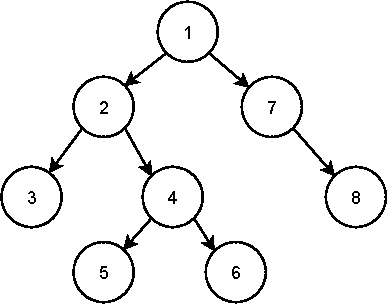
\includegraphics[width=0.48\textwidth]{obrazky-figures/ch2/DFS.pdf}
    \caption{Porovnání metod prohledávání stavového prostoru BFS (vlevo) a DFS (vpravo).}
    \label{fig:BFS_DFS}
\end{figure}

Prohledávání začíná v kořeni, neboli startovním uzlu, a postupně po úrovních, prochází prvně sousedy kořene, následně sousedy jeho sousedů, atd. dokud nedojde k cíli (zadaný hledaný uzel), od kterého navrátí nejkratší cestu až ke kořeni~\cite{Introduction_to_Algorithms}, či dokud neprohledá neúspěšně celý prostor. Výsledek prohledávání je možné vidět vlevo na obrázku~\ref{fig:BFS_DFS}.

Časová složitost je \(\mathcal{O}_{BFS} = |V| + |E|\), kde \(|V|\) je součet počtu uzlů a \(|E|\) je počet hran~\cite{CS225BFSDFS}.

\subsubsection*{\textbullet Metoda slepého prohledávání do hloubky (DFS)}
Metoda pracuje se zásobníkem LIFO (\textit{= last-in, first-out}), který využívá k~navrácení~\cite{poole2023artificial}. Stejně jako BFS začíná v kořeni, od kterého ale jde do hloubky. To znamená, že vybere jeden neprozkoumaný synovský sousední uzel, u kterého vybere jeho neprozkoumaný synovský sousední uzel a takto pokračuje, dokud nedorazí na \uv{dno}, tedy do místa, odkud již nelze dále pokračovat hlouběji\,--\,v tomto případě se navrátí k nejbližšímu otcovskému uzlu, u kterého ještě nebyly prozkoumány všechny synovské uzly a prohledává dál~\cite{Introduction_to_Algorithms}. Toto pokračuje, dokud nenalezne hledaný cílový uzel, nebo dokud neprojde celý prostor bez nalezení cíle. Ukázka průchodu stromem je v pravé části obrázku~\ref{fig:BFS_DFS}.

Stejně jako u BFS, časová složitost je \(\mathcal{O}_{DFS} = |V| + |E|\), kde \(|V|\) je součet počtu uzlů a \(|E|\) je počet hran~\cite{CS225BFSDFS}.

\subsubsection*{\textbullet Metoda postupného zanořování do hloubky (IDS)}
Tato metoda je kombinací BFS a DFS\,--\,prohledávání funguje stejně jako u~DFS s výjimkou, že algoritmus postupuje po úrovních a postupně si zvyšuje limit hloubky~\cite{poole2023artificial}. Při první iteraci prohledává hloubkově pouze první úroveň, poté co je celá prohledaná postupuje na druhou iteraci, při které už vstupuje i do druhé atd. dokud nenajde cíl, či nevyčerpá celý stavový prostor. 

IDS se využívá pokud nemůžeme stanovit hloubku řešení a jeho časová složitost je \(\mathcal{O}_{IDS}(b^{d})\), kde \(b\) je faktor větvení (průměrný počet následovníků uzlu) a \(d\) je hloubka optimálního řešení~\cite{izu}.

\begin{figure}[H]
    \centering
    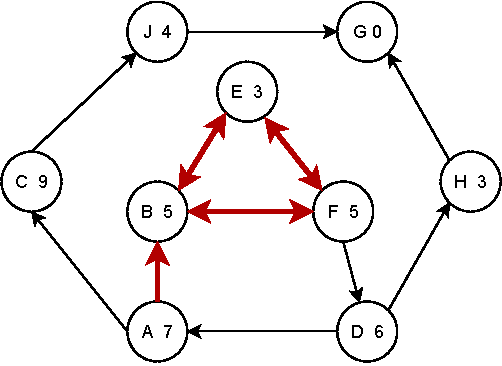
\includegraphics[width=0.7\textwidth]{obrazky-figures/ch2/GreedySearch.pdf}
    \caption{Nespolehlivost metody hladového prohledávání při hledání cesty z A do G, červeně zvýrazněno cyklení (uzly ve formátu [název uzlu, heuristika]).~\cite{poole2023artificial}}
    \label{fig:GreedySearch}
\end{figure}

\subsection*{Informované metody}
Informované metody na rozdíl od neinformovaných znají polohu cíle~\cite{izu}, kterou využívají na zhodnocení cesty pomocí funkce  ${f(n)}$, kde ${n}$ je stav/uzel. Tyto metody jsou také nazývány heuristickými, jelikož využívají k dosáhnutí cíle heuristickou funkci\,--\,díky této funkci ${h(n)}$ lze vypočítat pomocí uzlu ${n}$ nezáporné reálné číslo značící odhad nákladů na cestu z uzlu ${n}$~do uzlu cílového~\cite{poole2023artificial}. Čím menší je výsledné číslo, tím pravděpodobněji povede k cílovému uzlu a tedy ${h(n) = 0}$, ${n}$ je cílovým uzlem~\cite{AI-Modern_approach}.

\subsubsection*{\textbullet Metoda hladového prohledávání}
Anglicky nazývaný \textit{Greedy search}, je jeden z nejméně komplexních přístupů, jelikož využívá na zhodnocení uzlu pouze heuristickou funkci, tedy ${f(n) = h(n)}$~\cite{AI-Modern_approach}. Další krok od aktuálního uzlu se rozhoduje pouze v závislosti na této funkci, tedy hrana s nejmenší heuristikou, čímž může dojít k chybnému výsledku\,--\,metoda hladového prohledávání negarantuje nalezení výsledku~\cite{poole2023artificial}. 

Chybný postup k výsledku můžeme vidět v obrázku~\ref{fig:GreedySearch}, na kterém se nachází příklad z knihy \uv{Artificial Intelligence: Foundations of Computational Agents}~\cite{poole2023artificial}, kde při snaze o nalezení cesty z uzlu A do uzlu G zůstane algoritmus zacyklen v uzlech B, E, F.

\subsubsection*{\textbullet Metoda A*}
Metoda A* vyhodnocuje další krok na základě hodnotící funkce ${f(n) = g(n) + h(n)}$, kde ${g(n)}$ udává cenu cesty z předešlého do uzlu ${n}$ a ${h(n)}$ je heuristická funkce~\cite{AI-Modern_approach}. 

Pro správnou funkci A* algoritmu je důležité zvolit přípustnou (anglicky \textit{admissible}) heuristiku, což je heuristika, u které cena cesty z uzlu ${n}$ je spodním odhadem skutečné ceny k cíli~\cite{AI-Modern_approach, izu}. Jednou z přípustných heuristik, je přímá euklidovská vzdálenost mezi dvěma uzly~\cite{poole2023artificial}, která je vhodná na využití u prostorových problémů s přesnými rozměry (např. 2D mřížkový prostor bez překážek se čtyřmi povolenými směry\,--\,nahoru, dolu, doleva, doprava). Pokud algoritmus při jeho výpočtu dorazí k~výsledku heuristiky, která by toto nesplňovala, využívá \textit{backtracking}/navrácení a pokračuje v cestě k~dalšímu nejlepšímu uzlu.

Podobně jako u metody hladového prohledávání hledá algoritmus cestu po nejmenších hodnotách, ale díky využití kombinace ${g(n)}$ a ${h(n)}$ je algoritmus řazen jako optimální (vždy, když existuje, vrací optimální řešení)~\cite{poole2023artificial}.
    
%--------------------------
% Rejection sampling
\section{Rejection sampling}
Rejection sampling, či metoda accept-reject (česky přijetí-odmítnutí), je metoda vzorkování využívaná ke generování náhodných proměnných~\cite{thomopoulos2012essentials} a na vzorkování dat ze sofistikované neboli obtížně vzorkovatelné distribuce~\cite{Sachdeva_2021}.

Základní myšlenkou rejection samplingu je, že místo přímého vzorkování komplikované funkce f(X) můžeme generovat vzorky pomocí jednodušší distribuce Q(X) a následně zkontrolovat, zda patří do funkce komplikovanější~\cite{ghojogh2020sampling}. Na základě toho je poté lze přijmout, nebo odmítnout. Vizuální příklad je možné vidět na obrázku~\ref{fig:RA_graph}, který vyobrazuje vzorky vygenerované na základě funkce Q(X). Vzorky nacházející se v území patřící pod funkci f(X) a označené zelenou barvou budou akceptovány, kdežto body mimo (označené žlutě) jsou zamítnuty.

\vspace{0.3cm}
\begin{figure}[H]
    \centering
    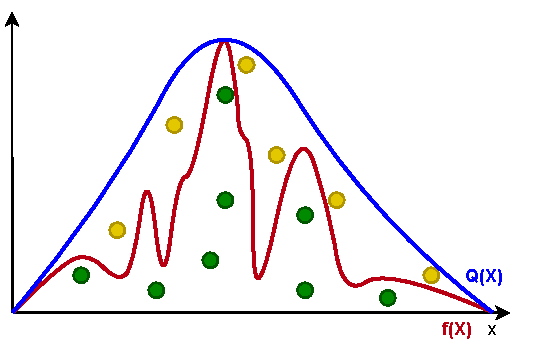
\includegraphics[width=\textwidth]{obrazky-figures/ch2/RA_graph.pdf}
    \caption{Příklad Rejection samplingu, kde jsou díky využití jednodušší distribuce Q(X) (modrá) získány vzorky ze složitější funkce f(X) (červená).}
    \label{fig:RA_graph}
\end{figure}
\vspace{0.3cm}

Pro detailnější vysvětlení je využit algoritmus~\ref{algo:rejection_sampling} sepsaný podle výukového a literárního přehledu z Univerzity Waterloo~\cite{ghojogh2020sampling} a edukační stránky~\cite{Sachdeva_2021}. V tomto algoritmu je $\mathcal{S}$ sada vzorkovacích dat o velikosti $n$, jež se postupně naplňuje generovanými daty, které jsou vzorky složitější funkce f(X). V cyklu generujícím a potvrzujícím vzorky je prvně vytvořen vzorek $x$ z funkce Q(X) a následně vzorek $u$ z rovnoměrného rozložení $U(0, c\, Q(x_i))$. Škálovací konstanta $c$ je využívána k určení horních mezí pro přijetí nebo odmítnutí vzorku a platí, že $c \cdot Q(x) \geq f(x) \ \text{pro všechny } x$.
\label{eq:RA_c}
\begin{algorithm}[h]
\caption{Rejection sampling/Accept-reject}\label{algo:rejection_sampling}
\begin{algorithmic}[1]
    \State \textbf{Input:} $f(x), Q(X), c$\;
    \State \textbf{Output:} $\mathcal{S}$
    \State $\mathcal{S} \gets \varnothing$
    \For{$i = 1$ to $n$}
        \State $x_i \sim Q(X)$
        \State $u_i \sim U(0, c\, Q(x_i))$
        \If{$u_i < f(x_i)$}
            \State Accept $x_i$: $\mathcal{S} \gets \mathcal{S} \cup \{x_i\}$
        \Else
            \State Reject $x_i$: $i \gets i - 1$
        \EndIf
    \EndFor
\end{algorithmic}
\end{algorithm}

%===---------------====
% KONCEPT
%===---------------====
\chapter{Koncept 2D labyrintové hry}\label{chap:Koncept 2D labyrintové hry}
Labyrintová hra ve svém pravém slova smyslu je hra, která umístí hráče do cizího prostředí, ze kterého se má za úkol dostat pryč. V základní verzi mu cestu ztěžují pouze slepé uličky. 

Toto téma ale v základu moc zájmu nepřiláká. Nejvíce populárních labyrintových her bylo vyvinuto jako původně arkádové hry v 80. letech 20. století a každá byla doplněna o~nějaký prvek/mechaniku, který je dělal zábavnější a hratelnější. Pac-Man například doplnil bloudění bludištěm o výzvu \uv{duchů}, tedy nepřátel pronásledujících hráče a dále sesbírání všech teček namísto hledání východu. Bomberman využil zajímavé mechaniky s~bombami, díky kterým se hráč zbavuje nepřátel a vytváří unikátní bludiště.

%--------------------------
% Úvod
\section{Fáze vývoje labyrintové hry}
K vývoji hry byly využity upravené postupy aspektů vývoje. Jelikož hra byla vytvářena pouze jednou osobou, tak k plánování a vývoji nebylo potřeba podrobných domluv s~několika týmy. Byla tedy odstraněna fáze \uv{preprodukce} a všechny potřebné věci byly promyšleny a otestovány ve fázi \uv{plánování}. Hru také nebylo v plánu komercializovat, což odstranilo fázi \uv{prelaunch}, jelikož pro hru nebylo potřeba vytvářet marketingový plán.

\subsection*{Plánování}
V této fázi byl vytvořen první návrh hry. Hlavním nápadem bylo vytvoření procedurálně generovaného bludiště pomocí celulárních automatů a popřípadě dalších algoritmů. Jeho cílem byla automatizace generování libovolně velkého hratelného bludiště, které ušetří lidskou práci na vývoji prostředí. Také by mělo přinést aspekt \uv{náhodnosti}, jelikož lidská bludiště mohou trpět na problémy repetitivnosti~\cite{Procedural_Game_Map}. Návrh vytváření tohoto bludiště je na obrázku~\ref{fig:navrh_generovani}.

Inspirace pro premisy hry byla brána z arkádových (\textit{skill-based}) her, v češtině her založených na dovednosti. Byl ponechán základní úkol\,--\,v bludišti se co nejrychleji zorientovat a~dojít k východu. V tom by hráči měli zabraňovat různí nepřátelé, se kterými může bojovat pro zisk vyššího skóre a bezstarostnější hledání cíle. V boji, přežití a pohybu v bludišti by mu měly pomoci různé předměty. Nápady na různé herní objekty jsou popsány důkladněji v~kapitole~\ref{chap:Herní mechaniky}.

Hra byla vytvořena jako produkt na počítač, konkrétně pro Windows a Linux. Kvůli svému žánru a povaze hra nemá příběh, ale je připravena hráče zabavit nápadem, výzvou a grafikou inspirovanou nostalgií a jednoduchostí arkádových pixelových her.

\begin{figure}[t]
    \centering
    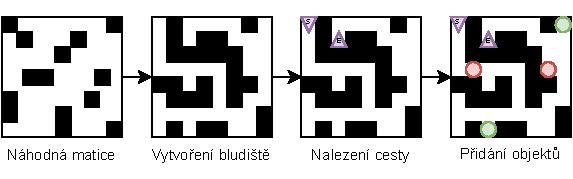
\includegraphics[width=0.96\textwidth]{obrazky-figures/ch3/navrh_generovani.pdf}
    \caption{Návrh automatizace generování bludiště.}
    \label{fig:navrh_generovani}
\end{figure}

\subsection*{Produkce}
Produkce hry byla rozdělena na několik etap. V první etapě byly vytvořeny algoritmy generující mapu a její start a cíl. Ty byly následně důkladně otestovány a byly vybrány nejlepší způsoby generování různých velikostí map pomocí různých algoritmů. Druhá etapa zahrnovala implementaci hráčské postavy, jejích textur a mechanik. Ve třetí etapě byly implementovány a animovány herní objekty jako jsou nepřátelé a předměty. Nakonec bylo naimplementováno GUI navržené pomocí programu \textit{Figma}.

Některé textury byly získány z internetu (stránky \textit{itch.io} pod licencí \textit{Creative Commons} a některé byly vytvořeny vlastnoručně. Použitý font je získaný ze stránky \textit{Google Fonts} pod licencí \textit{Open Font License}\,--\,více informací ke game assetům se nachází v README na přiloženém paměťovém médiu.

\subsection*{Testování}
Alfa verze hry (tedy \uv{feature complete}) byla zpřístupněna veřejnosti spolu s formulářem obsahujícím otázky technického charakteru a hratelnosti hry. Testeři mohli po ohodnocení hry přidat i svoje návrhy a nápady na zlepšení hry, ze kterých bylo několik vybráno a~implementováno. Detailnější popis testování a~jeho výsledků se nachází v kapitole~\ref{chap:Uživatelské testování}.


\subsection*{Publikace}
Pro plánovanou publikaci hry byla vybrána stránka \textit{itch.io}, nebo jí podobná platforma \textit{Game Jolt} a to kvůli jejich přívětivosti pro začínající herní vývojáře oproti známější a~populárnější herní platformě Steam. Ten totiž vyžaduje za publikaci poplatek ve výši 90~€~\cite{Steam_submission}. Tento poplatek je navrácen poté co hra dosáhne čistého zisku minimálně 1000~\$. Hra je ale plánována k vydání zdarma. Vydání hry na \textit{itch.io}, či \textit{Game Jolt} je naopak rychlé a~zdarma a~nabízí možnost lepšího propojení vývojáře s hráči a získávání zpětné vazby v~post-produkci, což z~ní dělá ideální platformu pro budoucí vývoj~\cite{GDevelop}. Populární platformou je také \textit{Epic Games}, ale pro publikaci musí hra projít náročným posouzením.

\subsection*{Postprodukce}
Je plánován budoucí vývoj hry i po dokončení práce. Do hry by mohly přibýt nové mechaniky či herní módy a budou opravovány nalezené chyby.

%--------------------------
% Herní mechaniky
\section{Herní mechaniky}\label{chap:Herní mechaniky}
Jak už bylo zmíněno výše, hlavní myšlenkou hry je hráč procházející nekonečné množství ztěžujících se bludišť. V tom mu budou bránit nepřátelé, pomáhat sbíratelné předměty a~za úspěšné dokončení mu bude uděleno skóre.

\begin{figure}[h]
    \centering
    \vspace{0.3cm}
    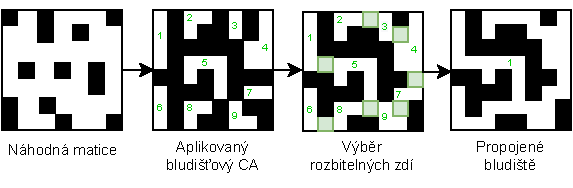
\includegraphics[width=\textwidth]{obrazky-figures/ch3/algoritmus_generovani_mapy.pdf}
    \caption{Návrh algoritmu pro generování mapy bludiště.}
    \label{fig:algoritmus_generovani_mapy}
\end{figure}

\subsection*{Bludiště}
Hlavním problémem je řešení rychlého generování diverzních 2D bludišť. Díky tomu, že jsou dvoudimenzionální, je možné na jejich zobrazení využít matici o 2 náhodně vygenerovaných hodnotách\,--\,jedna hodnota symbolizující políčka zdí bludiště a druhá symbolizující políčka cest. Náhodný výběr hodnot vytvoří ideální základ pro další algoritmy použité při generování bludiště.

Pro využití generovaných bludišť ve hrách je potřeba jejich rychlého vytváření. Pokud by totiž hra, která je založená primárně na bludištích, generovala každé z nich byť i jen několik sekund, pro hráče by to nebyl pozitivní \uv{user experience}. Proto jsou k hlavnímu vývoji využity relativně rychlé celulární automaty. Jak je vidět na obrázku~\ref{fig:OCA:Maze}, z kapitoly~\ref{chap:Celulární automaty}, CA Mazectric generující bludiště vytváří pouze strukturu podobnou bludišti. Proto je důležité vymyslet algoritmus pro propojení všech vytvořených místností do jedné jediné. Vybraným přístupem je vyhledat všechny vytvořené místnosti a postupně odstraňovat náhodné zdi, které je propojují\,--\,tím se algoritmus postupně dostane k bodu, kdy je v celém bludišti už jen 1 velká pospojovaná místnost. Vizualizace postupu tohoto algoritmu se nachází na obrázku~\ref{fig:algoritmus_generovani_mapy}.

Problém CA Mazectric je, že na velkých plochách vytváří zbytečně moc místností, které by bylo algoritmicky náročné a zdlouhavé propojovat. Proto je na tyto větší místnosti při generování využit CA generování jeskyní jakožto mezistupeň mezi náhodnou maticí a~Mazectric CA. Ten tvoří shluky bodů, jenž jsou následně rozgenerovány bludišťovým CA, které na velkých plochách přichází k lepším výsledkům. To díky tomu, že je \uv{explozivní}, což znamená, že většinou náhodně
vygenerované počáteční vzory explodují do všech směrů, což vytváří malý počet delších a větších chodeb.

Následně je potřeba v bludišti určit začátek a konec. Je možné vzít 2 náhodné body, každý na jiné straně bludiště. To ale může přinést problém, že tyto 2 body jsou propojené přímou, krátkou a nesložitou cestou, takže dosažení cíle nepředstavuje moc velkou výzvu. Pro zvýšení obtížnosti je vhodné využít algoritmus vyhledávající 2 co nejvzdálenější body v celém bludišti. K tomu se využívají neinformované metody, konkrétně metoda slepého prohledávání do šířky. Opakované prohledávání bludiště by ale způsobilo zpomalení generovacího algoritmu, proto bude BFS nad bludištěm spuštěn pouze dvakrát, pro nalezení optimálního startu a cíle, jak pro hráčskou výzvu, tak výpočetní algoritmus.

\subsection*{Úrovně a zvyšování složitosti}
Pro zvyšování složitosti videohry bylo vybráno několik prvků, které přinášejí postupně narůstající výzvu pro hráče. Jeden z těchto prvků spočívá v postupném zvětšování rozměrů bludiště během hraní. Hráč v úrovni 1 začíná na relativně malém čtvercovém bludišti. Po úspěšném dokončení této úrovně se přesouvá do bludiště o rozměrech $(x + 1) \times (x + 1)$ a~tak dále. Tento přístup vytváří pro hráče progresivně obtížnější prostředí se stále delšími cestami k~cíli a větším množstvím slepých cest, čímž poskytuje neustále rostoucí výzvu a~napětí.

Dalším prvkem, který přidává do hry narůstající výzvu, je postupně se zvyšující počet nepřátel a pastí v bludišti, které brání hráči v dosažení cíle. Na začátku hry se hráč nesetká s~žádnými překážkami, aby se seznámil s~principy hry, ale jakmile tyto úrovně dokončí, začnou se v bludišti objevovat nepřátelé a pasti. Jejich počet bude postupně narůstat lineárně, což ztěžuje hráči průchod bludištěm a přidává napětí do hry.

Kromě nepřátel se v bludišti také objevují předměty, které mohou hráči pomoci. Jejich výskyt následuje podobný trend jako u nepřátel, tedy s lineárním vzestupem v závislosti na úrovni hry.

Získání pozic pro místa, kde se budou objevovat nepřátelé či objekty je nutné brát v~potaz diverzní vývoj bludiště. Proto nemůžou být zvoleny fixní body či oblasti pro zjevování nepřátel. V reakci na to byla zvolena metoda zvaná rejection sampling. Tato metoda přináší možnost volného náhodného výběru políček z prázdné vzorkové matice (o stejné velikosti jako bludiště) na kterých je možnost položení entity. Tato matice je následně překryta s maticí bludiště a políčka potenciálního bodu pro entitu překrývající se s políčky cesty mohou být posunuty další funkci\,--\,na obrázku~\ref{fig:rozmisteni_rs} jsou zvýrazněna zelenou barvou. Ta si převezme potřebný počet souřadnic, které potřebuje přiřadit entitám.

\begin{figure}[b]
    \centering
    \vspace{0.5cm}
    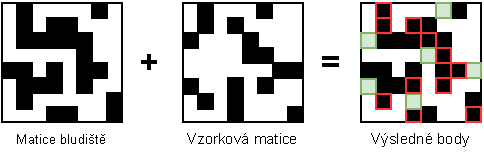
\includegraphics[width=\textwidth]{obrazky-figures/ch3/rozmisteni_rs.pdf}
    \caption{Návrh algoritmu pro rozmístění entit (zelená políčka označují možná využitelná místa).}
    \label{fig:rozmisteni_rs}
\end{figure}


\subsection*{Skóre}
Za dokončení každé úrovně hráč získá jako odměnu Body připočítávající se k jeho celkovému skóre. Body jsou počítány z jeho úrovně, kterou je násobena konstanta symbolizující dokončení bludiště, od kterého je ale odečteno, jak dlouho hráči trvalo úroveň dokončit. Cílem toho je motivovat hráče dokončit úroveň co nejrychleji. Zvyšování odměny za úspěšné dokončení úrovně je implementováno kvůli zvětšující se velikosti bludiště a tedy i zvyšujícímu se času na jeho dokončení.

Dále hráč získá body za zabití nepřátel a sběr předmětů, popřípadě bonusové předměty (viz Předměty). Podobně jako u dokončení úrovně, bude tato hodnota označena konstantou a~násobena úrovní. Násobením těchto konstant se zaručuje udržení stejného ocenění získané odměny, ať už hráč zabije nepřítele na úrovni 5 či na úrovni 20. \\
\newline
\noindent Z těchto podmínek byla zhotovena rovnice:

\begin{equation}
    \text{Skóre} = (\text{L} \times \alpha) - \text{t} + (\text{E} \times \beta) + (\text{I} \times \delta) + \textit{Bonus}
    \label{eq:default_score}
\end{equation}

\noindent kde:
\begin{flalign*}
    &&&\text{L} && := \text{úroveň bludiště}, & \\
    &&&\alpha && := \text{koeficient odměny za dokončení úrovně}, & \\
    &&&\text{t} && := \text{čas strávený na úrovni}, & \\
    &&&\text{E} && := \text{počet nepřátel, které hráč porazil}, & \\
    &&&\beta && := \text{koeficient  odměny za poražené nepřátele}, & \\
    &&&\text{I} && := \text{počet předmětů, které hráč sebral}, & \\
    &&&\delta && := \text{koeficient odměny za sebrané předměty}, & \\
    &&&\textit{Bonus} && := \text{případný bonus}. &
\end{flalign*}


\subsection*{Hráč}
Pro simulaci bloudění v bludišti bylo vybrán pohled na hráčskou postavu z 3. osoby s~omezením pohledu na pouze malé okno (například 5×5 bloků). Vykreslování celého bludiště by totiž bylo moc složité s ohledem na jeho zvětšující velikost. Naopak ponechaní výřezu, ale zvětšení pohledu na hráče (např. 10×10 bloků) by bylo moc matoucí a ničilo by to výzvu nižších úrovní, jelikož by hráč viděl většinu bludiště již při startu.

Hráč začíná s fixním počtem životů, který je možno zvýšit, ale jen do stanoveného maxima. Jako bonus může získat i štít, jenž nuluje jeden útok. Může útočit na blízko a díky předmětům lze zvýšit zranění, které způsobuje.

Hráčská postavička může být ovládána jak tlačítky WASD, tak i klávesami šipek pro vyhovění širší hráčské základně\,--\,toto by mělo fungovat bez zbytečného přepínání v nastavení, pro volnost předávání hry mezi více hráči.

\subsection*{Nepřátelé a pasti}
Pro zvýšení rozmanitosti a výzvy pro hráče bylo do hry přidáno několik různých nepřátel a pastí, každý s vlastními speciálními schopnostmi a vlastnostmi. V tabulce~\ref{tab:nepritele} lze nalézt seznam nepřátel, zatímco v tabulce~\ref{tab:pasti} jsou uvedeny pasti. Tyto prvky přinášejí hráčům pestrou škálu výzev a strategických možností, na než musí být při průchodu bludištěm připraveni, jelikož nikdy neví, který z nepřátel se v daném bludišti objeví.

\begin{table}[ht]
    \centering
    \begin{tabular}{|m{2cm}|m{2cm}|m{8cm}|}
    \hline
    \multicolumn{1}{|c|}{\textbf{Obrázek}} & \multicolumn{1}{c|}{\textbf{Jméno}} & \multicolumn{1}{c|}{\textbf{Popis schopnosti}} \\
    \hline
    \hline
    \centering
\includegraphics[width=1.5cm,height=1.5cm]{obrazky-figures/ch3/demon.png} & Démon & V intervalech zapaluje zem pod sebou (viz past \uv{Oheň}). \\
    \hline
    \centering
\includegraphics[width=1.5cm,height=1.5cm]{obrazky-figures/ch3/goblin.png} & Goblin & Nepřítel na dálku, jeho zbraní je luk\,--\,střílí šípy. \\
    \hline
    \centering
\includegraphics[width=1.5cm,height=1.5cm]{obrazky-figures/ch3/skeleton.png} & Kostlivec & Rychlý nepřítel. \\
    \hline
    \centering
\includegraphics[width=1.5cm,height=1.5cm]{obrazky-figures/ch3/slime.png} & Slime & Jeho útok hráči na krátkou dobu sníží rychlost. \\
    \hline
    \centering
\includegraphics[width=1.5cm,height=1.5cm]{obrazky-figures/ch3/yeti.png} & Yeti & V intervalech staví sněhuláky (viz past \uv{Sněhulák}). \\
    \hline
    \end{tabular}
    \caption{Popis nepřátel a jejich schopností.}
    \label{tab:nepritele}
\end{table}

\vline

\begin{table}[H]
    \centering
    \begin{tabular}{|m{2cm}|m{2cm}|m{8cm}|}
    \hline
    \multicolumn{1}{|c|}{\textbf{Obrázek}} & \multicolumn{1}{c|}{\textbf{Název}} & \multicolumn{1}{c|}{\textbf{Popis vlasnosti}} \\
    \hline
    \hline
    \centering
\includegraphics[width=1.5cm,height=1.5cm]{obrazky-figures/ch3/fire.png} & Oheň & Pokud na něj hráč vstoupí, zapálí se (ubírá mu postupně životy). Po určité době vyhasne. \\
    \hline
    \centering
\includegraphics[width=1.5cm,height=2cm]{obrazky-figures/ch3/snowman.png} & Sněhulák & Blokuje hráči cestu, postupně se rozpouští a~může být zničen hráčem. \\
    \hline
    \centering
\includegraphics[width=1.5cm,height=2cm]{obrazky-figures/ch3/trap.png} & Vysunovací bodáky & V intervalech se aktivují\,--\,pokud na ně hráč stoupne v aktivním stavu uberou mu životy. \\
    \hline
    \end{tabular}
    \caption{Popis pastí a jejich vlastností.}
    \label{tab:pasti}
\end{table}

\subsection*{Předměty}
Do hry bylo dále přidáno několik předmětů, které hráči pomáhají v boji, přežití nebo prozkoumávání bludiště. V tabulce~\ref{tab:přeměty} se nachází seznam těchto předmětů spolu s bonusy, které poskytují hráči. Tyto předměty přidávají do hry další strategické možnosti a posilují hráčovu schopnost překonat výzvy, jež mu bludiště přináší.

\begin{table}[htbp]
    \centering
    \begin{tabular}{|m{2cm}|m{2cm}|m{8cm}|}
    \hline
    \multicolumn{1}{|c|}{\textbf{Obrázek}} & \multicolumn{1}{c|}{\textbf{Název}} & \multicolumn{1}{c|}{\textbf{Popis bonusu}} \\
    \hline
    \hline
    \centering
\includegraphics[width=1.3cm,height=1.3cm]{obrazky-figures/ch3/green_potion.png} & Lektvar zrychlení & Permanentně hráči zvýší rychlost. \\
    \hline
    \centering
\includegraphics[width=1.3cm,height=1.3cm]{obrazky-figures/ch3/red_potion.png} & Lektvar zdraví & Vyléčí hráči několik životů. \\
    \hline
    \centering
\includegraphics[width=1.3cm,height=1.3cm]{obrazky-figures/ch3/chests.png} & Truhla & Přidá hráči bonusové skóre. \\
    \hline
    \centering
\includegraphics[width=1.3cm,height=1.3cm]{obrazky-figures/ch3/shield.png} & Štít & Přidá hráči štít. \\
    \hline
    \centering
\includegraphics[width=1.3cm,height=1.7cm]{obrazky-figures/ch3/sword.png} & Meč & Permanentně hráči zvýší poškození, které uděluje nepřátelům.\\
    \hline
    \end{tabular}
    \caption{Popis předmětů a jejich bonusů.}
    \label{tab:přeměty}
\end{table}

%--------------------------
% Uživatelské rozhraní
\section{Uživatelské rozhraní}
Uživatelské rozhraní bylo navrženo v programu Figma s důrazem na jednoduchost a inspiraci z arkádových her. Proto byla použita simplistická barevná paleta textur a pixelové entity (viz obrázek~\ref{fig:end_level_game}). Cílem hry je dosáhnout co nejvyššího skóre. Hráč má možnost porovnat své výsledky ve výpisu nejvyšších skóre, jako je vidět na obrázku~\ref{fig:score_screen}. Na tuto obrazovku se dostane z menu, jež je zobrazeno na stejném obrázku. Návrh je také zaměřen na uživatelskou přívětivost, proto je ve hře stránka s návodem a příručkou k herním entitám. Dále jsou také implementované potvrzovací vyskakovací okénka zabraňující mylným překlikům (obrázek~\ref{fig:information_screen}). 

Pro samotnou hru bylo navrženo okno s čtvercovým pohledem kamery na hrací pole, které mění motivy v závislosti na úrovni. Na pravém a levém boku okna jsou umístěny hráčské životy a štíty spolu s aktivními bonusy. Tím vytváří nerozptylující a vyvážený symetrický pohled, který je možno vidět na obrázku~\ref{fig:game_screen}.

\begin{figure}[hb]
    \vspace{0.2cm}
    \centering
    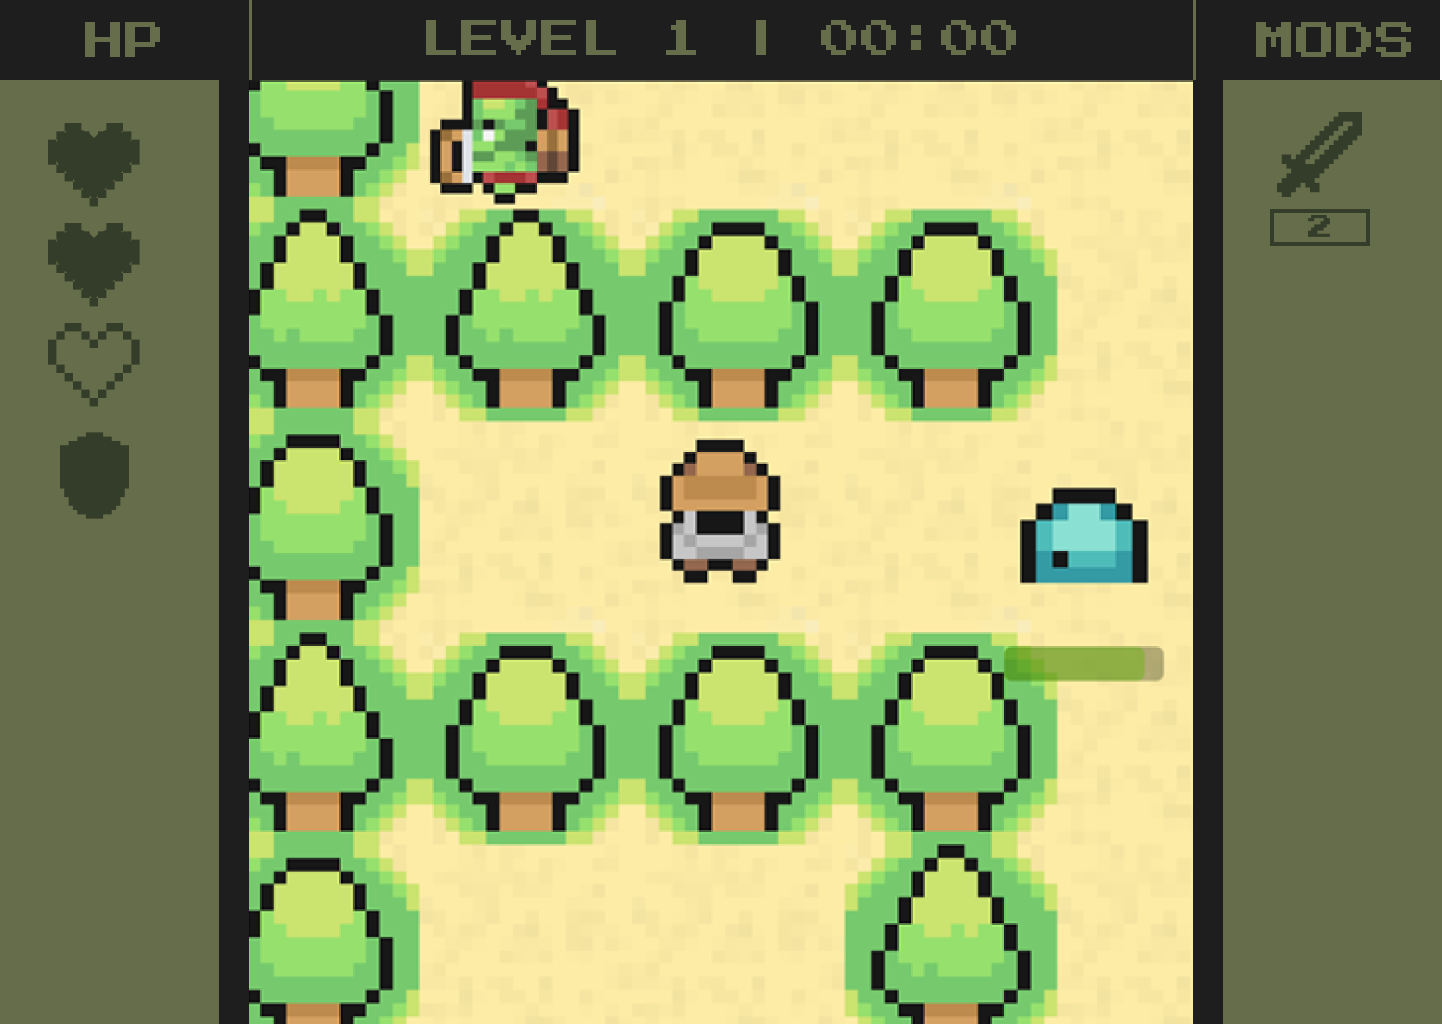
\includegraphics[width=0.44\textwidth]{obrazky-figures/ch3/game_screen.png}\hspace{0.1cm}
    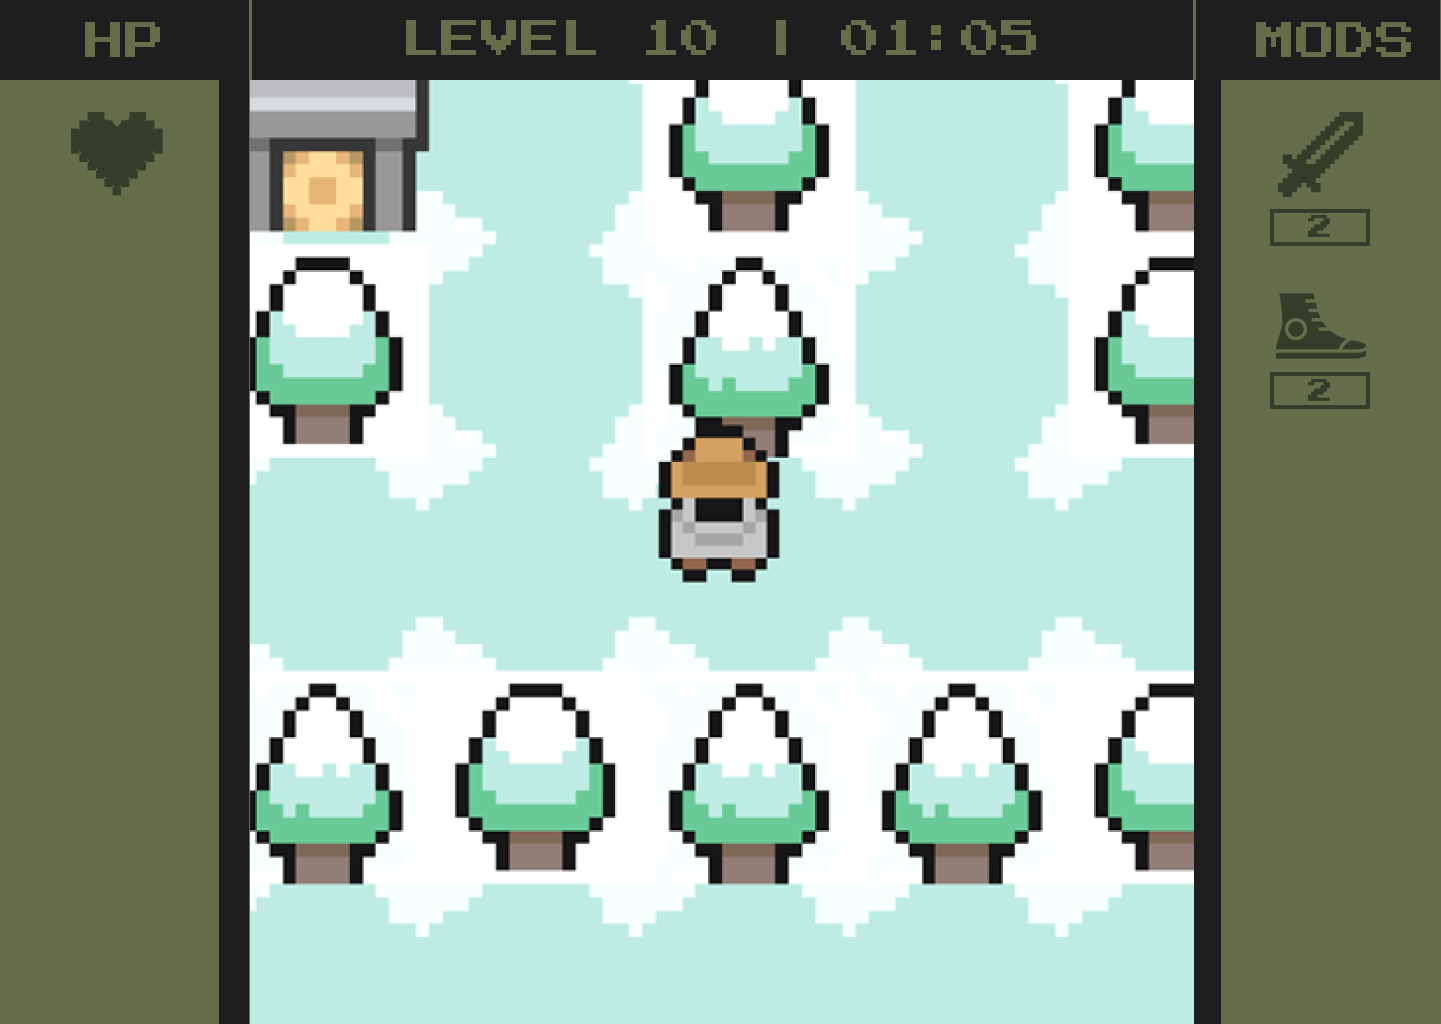
\includegraphics[width=0.44\textwidth]{obrazky-figures/ch3/Game_screen-WINTER_BLOCK.png}
    \caption{Ukázka návrhu herní obrazovky z Figma.}
    \label{fig:game_screen}
\end{figure}


\begin{figure}[H]
    \centering
    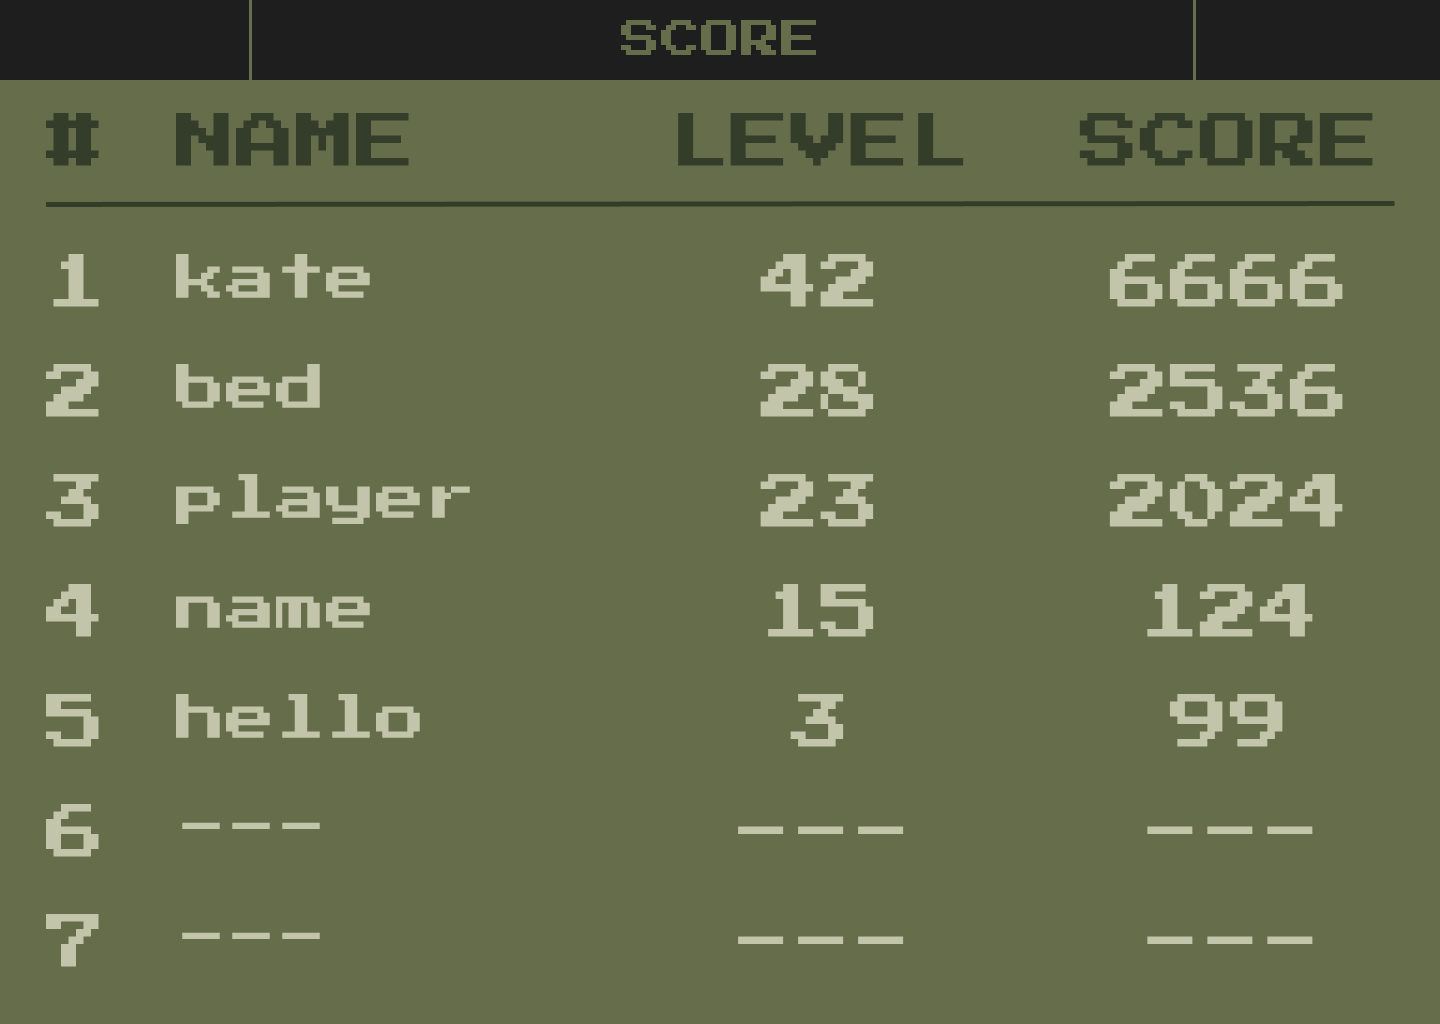
\includegraphics[width=0.42\textwidth]{obrazky-figures/ch3/Score_screen.png}\hspace{0.1cm}
    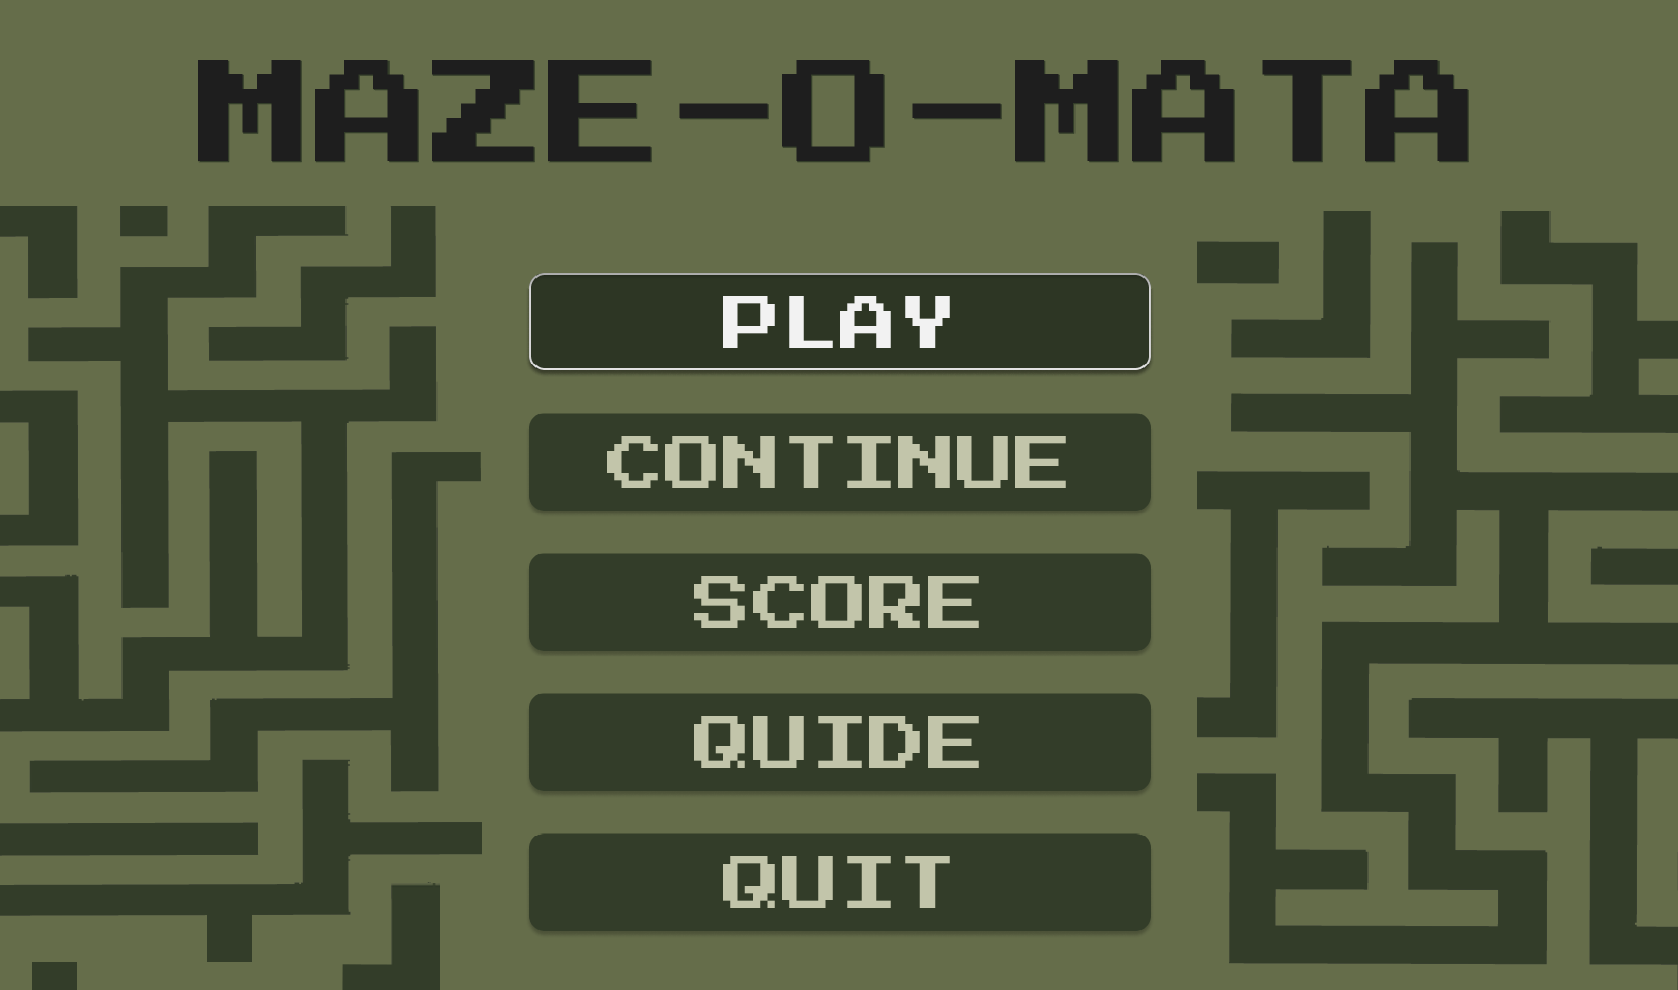
\includegraphics[width=0.505\textwidth]{obrazky-figures/ch1/game_menu.png}
    \caption{Ukázka návrhu herní obrazovky z Figma\,--\,výpis nejvyšších skóre (vlevo) a~hlavní menu (vpravo).}
    \label{fig:score_screen}
\end{figure}


\begin{figure}[H]
    \centering
    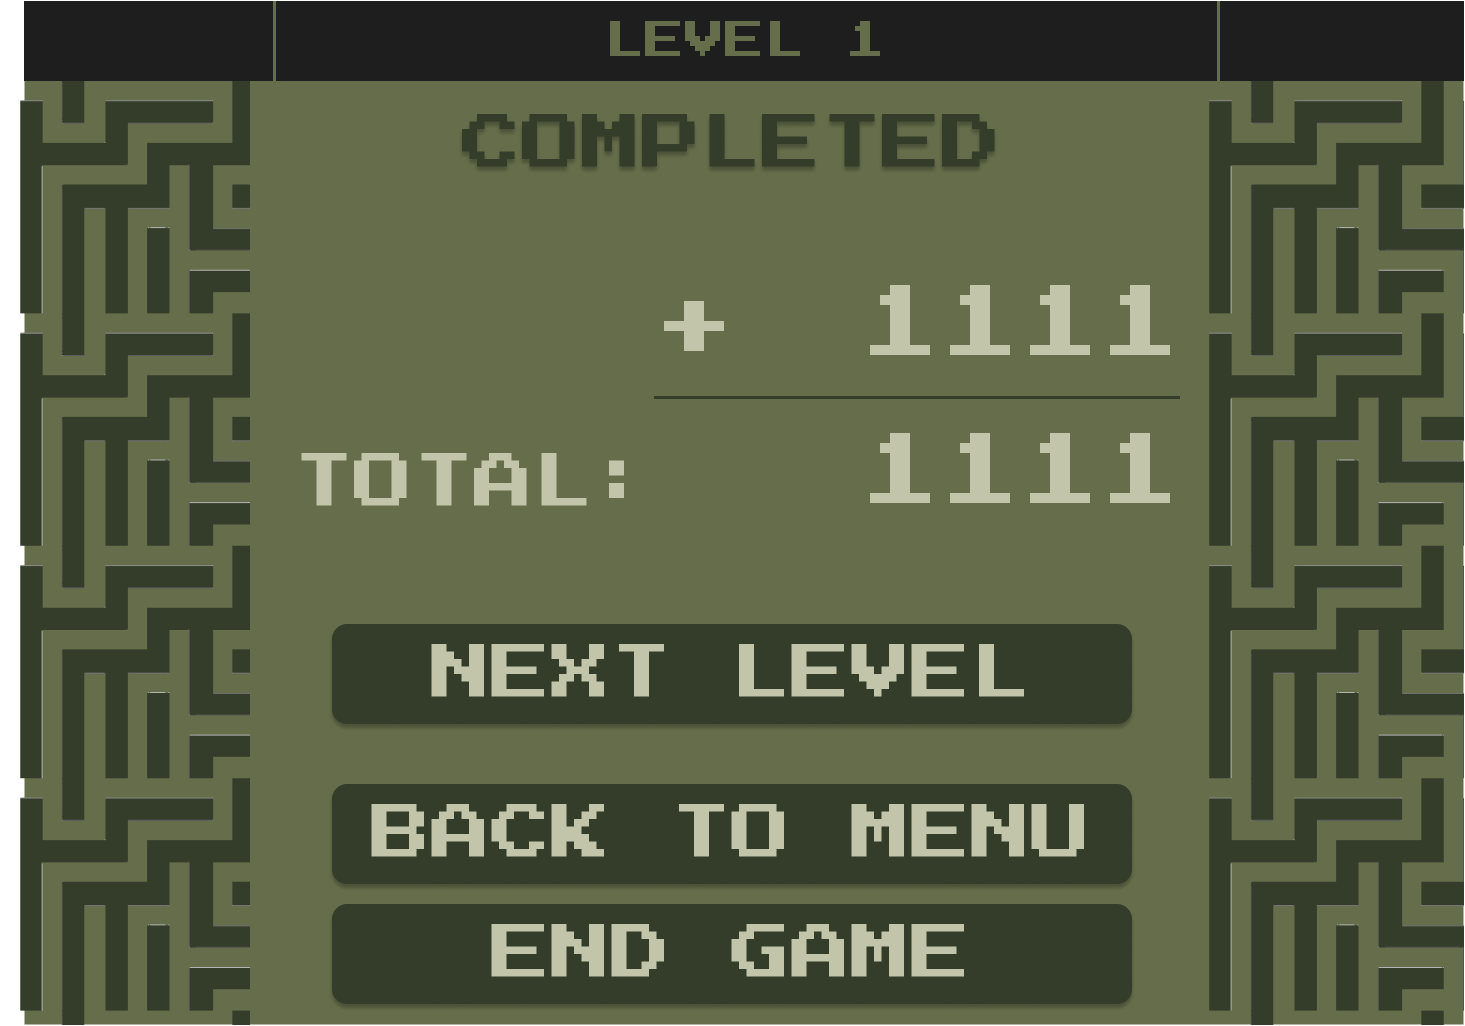
\includegraphics[width=0.482\textwidth]{obrazky-figures/ch3/level_completed_screen.png}\hspace{0.1cm}
    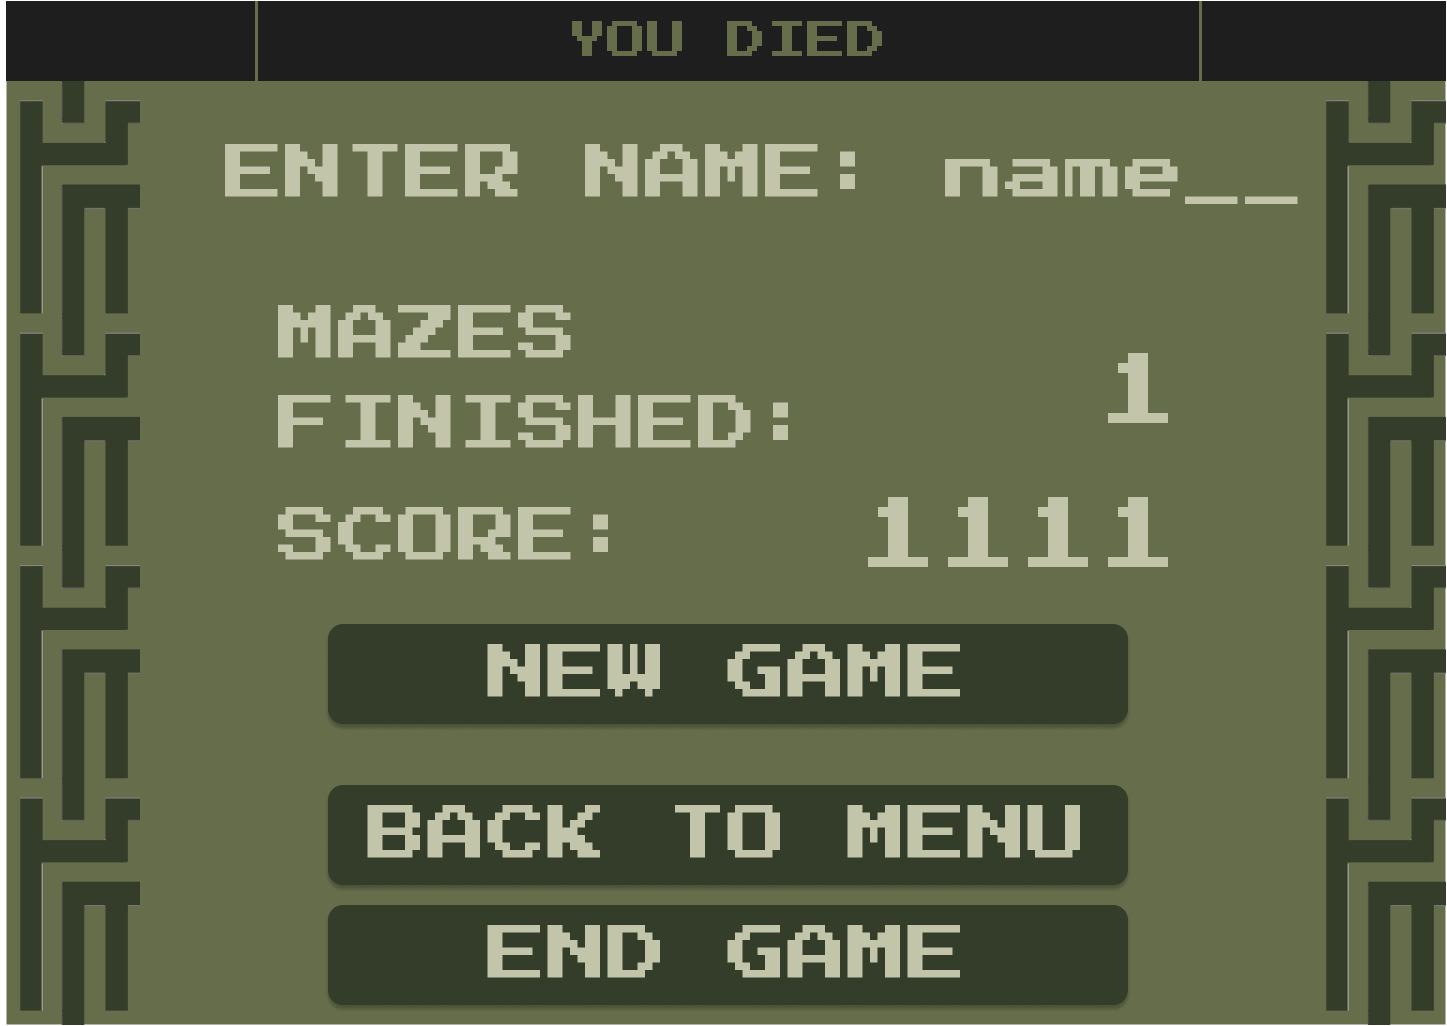
\includegraphics[width=0.48\textwidth]{obrazky-figures/ch3/end_game_screen.png}
    \caption{Ukázka návrhu z Figma\,--\,na levé straně se nachází obrázek úspěšně dokončené úrovně a na pravé hry prohrané.}
    \label{fig:end_level_game}
\end{figure}


\begin{figure}[H]
    \centering
    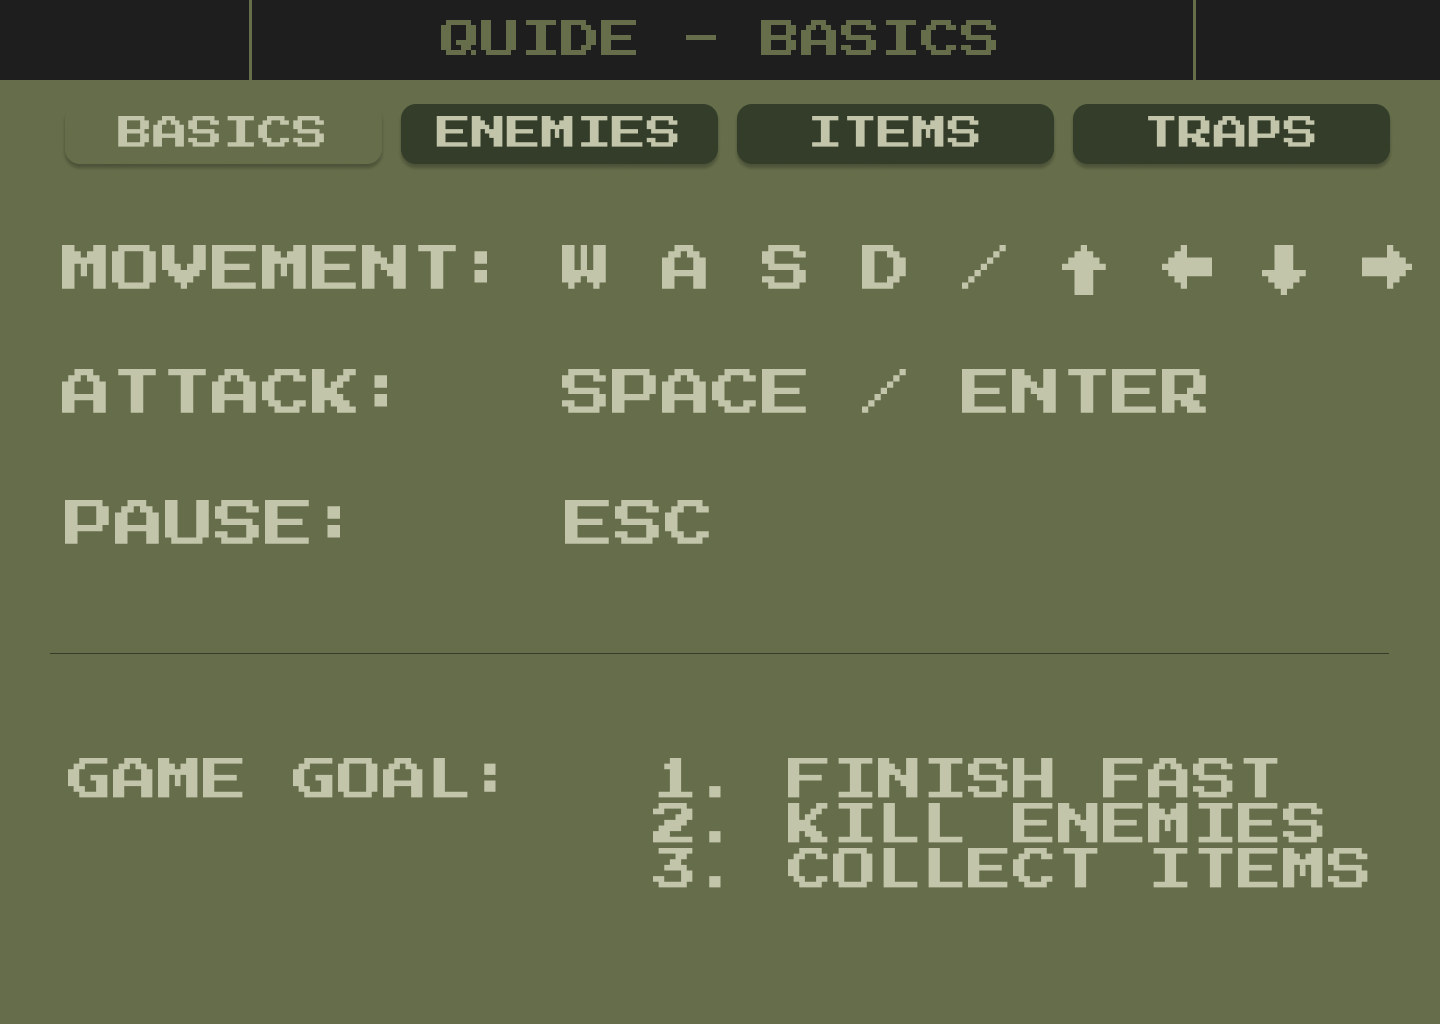
\includegraphics[width=0.48\textwidth]{obrazky-figures/ch3/Quide - Basics.png}\hspace{0.1cm}
    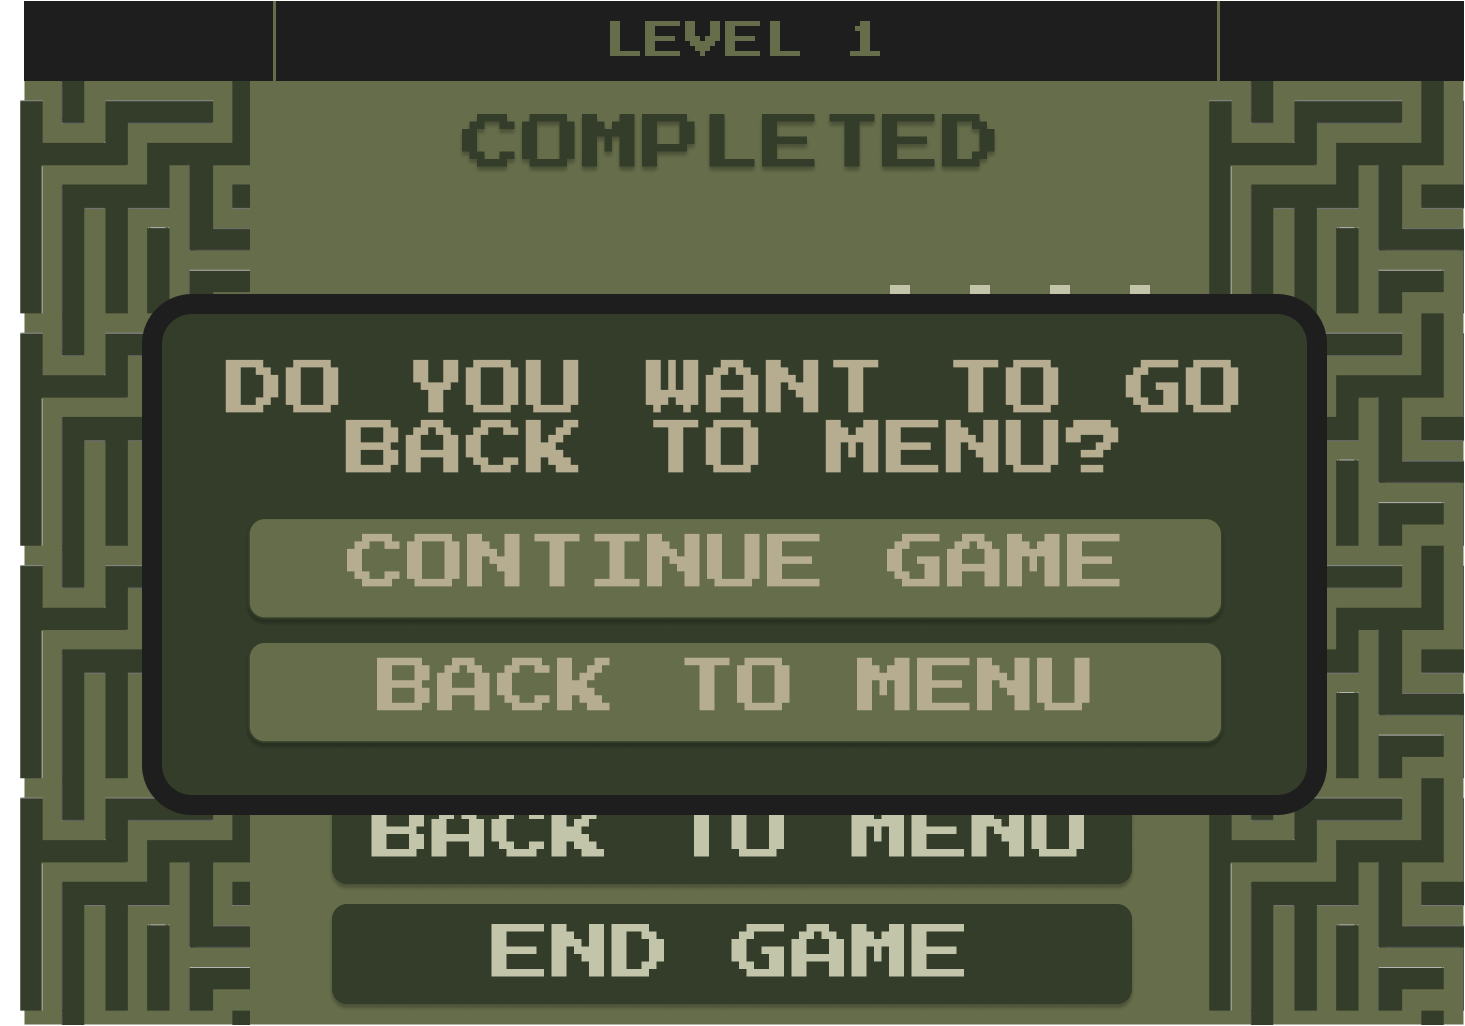
\includegraphics[width=0.486\textwidth]{obrazky-figures/ch3/level_completed_affirming_menu.png}
    \caption{Ukázka návrhu z Figma\,--\,na levé straně se nachází obrázek z nápovědy a na pravé potvrzovací obrazovka.}
    \label{fig:information_screen}
\end{figure}

%===---------------====
% IMPLEMENTACE
%===---------------====
\chapter{Tvorba bludiště a realizace hry}\label{Tvorba bludiště a realizace hry}
Pro implementaci hry bylo otestováno několik game enginů a zváženy jejich výhody a nevýhody. Jelikož cílem bylo vytvořit jednoduchou 2D hru, jejíž hlavním a nejsložitějším bodem je mapa byl vybrán Godot 4. 

Tato platforma byla zvolena oproti jiným možnostem díky její široké a jednoduché podpoře vytváření 2D her. Unreal Engine nebyl vybrán, protože je zaměřený spíše na realistické 3D světy. Jak je již zmíněno v kapitole o Godotu, tento herní engine na rozdíl od Unity či Unreal Enginu využívá vlastní skriptovací jazyk GDScript, podobný syntaxí pythonu, který díky svým knihovnám ulehčuje manipulaci s herními prvky (nodes) a urychluje tak vývoj.

Hru strukturovala řada funkčních prvků, které dohromady tvoří celkový koncept hry. Podrobnější popis implementace některých z těchto prvků je uveden v následujících částech této kapitoly. Schéma propojení mezi těmito skupinami je zobrazeno na obrázku~\ref{fig:schema_hry}.

\begin{figure}[H]
    \centering
    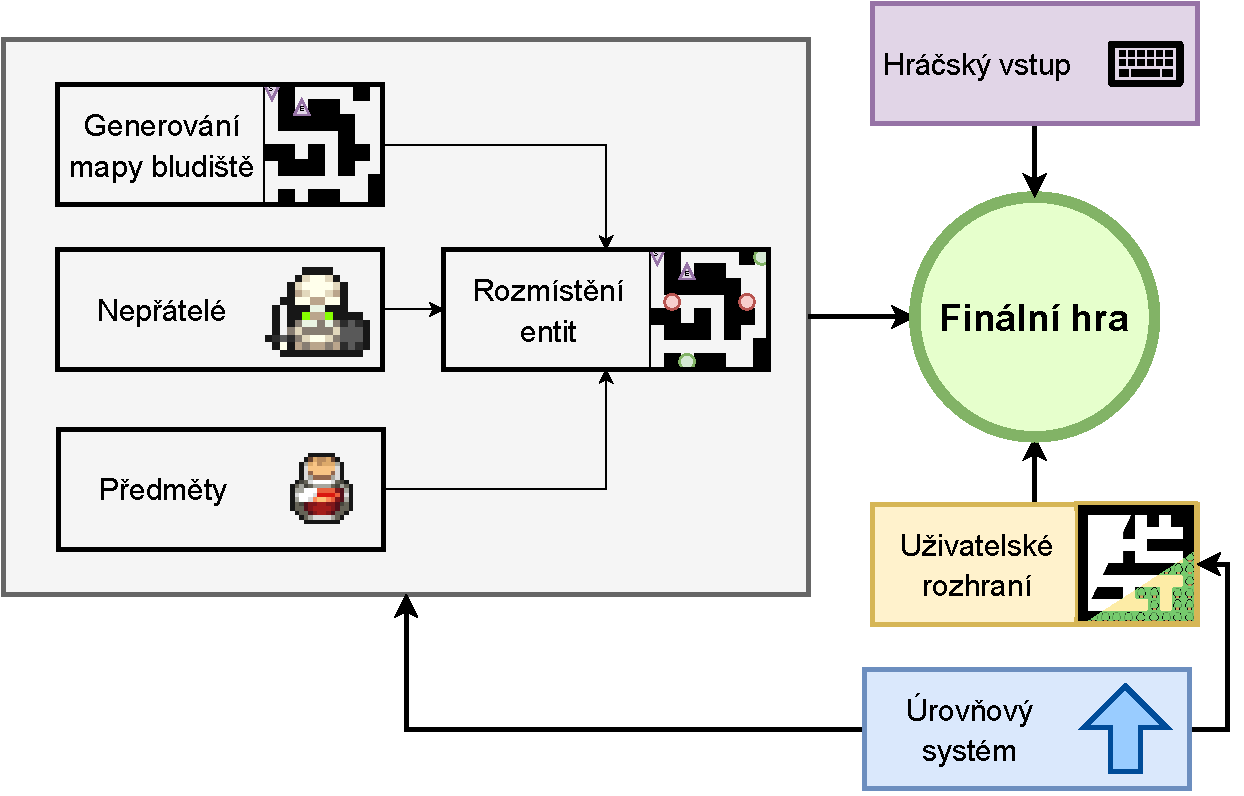
\includegraphics[width=\textwidth]{obrazky-figures/ch4/blokove_schema_hry.pdf}
    \caption{Blokové schéma ukazující závislosti hlavních prvků hry.}
    \label{fig:schema_hry}
\end{figure}

%--------------------------
% Generování mapy
\begin{figure}[ht]
    \centering
    \begin{minipage}[c]{0.48\textwidth}
        \centering
        \[
        \begin{bmatrix}
            1 & 0 & 1 & 1 & 0 & 1 & 0 \\
            0 & 0 & 0 & 0 & 0 & 1 & 0 \\
            1 & 1 & 0 & 1 & 1 & 1 & 0 \\
            0 & 0 & 0 & 0 & 0 & 1 & 0 \\
            1 & 0 & 1 & 1 & 0 & 0 & 0 \\
            0 & 0 & 0 & 1 & 0 & 1 & 0 \\
            0 & 1 & 0 & 1 & 0 & 1 & 0 \\
        \end{bmatrix}
        \]
    \end{minipage}
    \begin{minipage}[c]{0.48\textwidth}
        \centering
        
\includegraphics[width=0.8\textwidth]{obrazky-figures/ch4/matrix_to_maze.pdf}
    \end{minipage}
    \caption{Ukázka převodu matice na mapu.}
    \label{fig:matrix_to_maze}
\end{figure}
\vspace{1.3cm}

\section{Generování mapy}
Jakožto podklad 2D mapy byla vybrána matice o pevné velikosti $x \times y$, značící rozměry mapy. Obsah této matice reprezentuje strukturu bludiště (bez hraničních stěn). Každá buňka této matice může obsahovat hodnotu 1 nebo 0, kde hodnota 1 označuje zeď a hodnota 0 průchodnou cestu. Volba matice byla provedena z důvodu kompatibility s vizuálním prvkem Godotu TileMap, jenž ulehčuje vykreslování 2D herního pole. Ten umožňuje převést hodnoty matice na konkrétní pozice na mapě do dlaždic, jak je vidět na obrázku~\ref{fig:matrix_to_maze}. Takto lze jednoduše definovat strukturu bludiště pomocí algoritmů na matici a následně ji jen zobrazit prostřednictvím prvku TileMap.

V následující části je po krocích (vizualizovaných v obrázku~\ref{fig:visualisation_generating}) popsáno generování bludiště optimalizované pro tvoření bludišť pro implementovanou hru. První úroveň bude mít kostku o rozměrech $7 \times 7$, což je optimální velikost pro hráče, aby se snáze naučili ovládání hry a pochopili její cíl. Tato velikost také, díky důkladnému testování, zaručuje, že v žádném testu nedojde ke vzniku prázdné nebo nulové matice. Menší velikosti měly občasné problémy s generováním prázdných ploch (nulových matic). Jak již bylo navrhnuto v konceptu, každá další úroveň zvětší oba rozměry bludiště o 1.

\vspace{0.5cm}
\begin{figure}[b]
    \centering
    \includegraphics[width=\textwidth]{obrazky-figures/ch4/visualisation_generating.pdf}
    \caption{Programová vizualizace postupných výsledků generování bludiště}
    \label{fig:visualisation_generating}
\end{figure}

\subsection*{Kostra bludiště}
Na základě testů, které jsou popsané v další podkapitole~\ref{chap:Experimenty s generováním map}, byly vyhodnoceny 3 velikostní skupiny pro generování bludišť\,--\,malé (\verb|SMALL|), střední (\verb|MEDIUM|) a velké (\verb|LARGE|). Ty se od sebe liší drobnostmi ve způsobu generování kostry, tedy nepropojené navržené části bludiště.

Prvním krokem v generování bludiště je vytvoření náhodné matice, nad kterou budou později spuštěné celulární automaty. To je zařízeno díky nativnímu generátoru pseudo-náhodných čísel \verb|randi| v Godotu. Ten pracuje na základě PCG (Permuted Congruential Generator), který umožňuje vytvářet pseudonáhodná čísla s vylepšenými statistickými vlastnostmi díky kombinaci kongruentního generátoru a permutací~\cite{PCG}. 

Výsledky generátoru čísel funkce \verb|randi| (jenž vrací náhodné celé číslo) jsou transformovány do matic pomocí operace modulo 2, což zajistí, že matice obsahují pouze hodnoty 1~nebo 0. Tato technika je využita pro matice označené jako \verb|SMALL| a \verb|MEDIUM|. Pro bludiště typu \verb|LARGE| je použita složitější metoda, která zahrnuje dva kroky. Nejprve je výsledek operace \verb|randi| modulován číslem 3 a poté je výsledek této operace modulován ještě jednou číslem 2. Tento postup zajišťuje, že výsledná matice obsahuje více nulových hodnot (které reprezentují cesty) než jedničkových (které reprezentují zdi), a to v poměru 2:3. Tím je dosaženo optimálnějšího generování bludiště. Srovnání vizuálního výstupu obou metod generování je zobrazeno na obrázku~\ref{fig:randi}.

Náhodná matice je následně předána celulárním automatům. Matice reprezentující bludiště typů \verb|LARGE| a \verb|MEDIUM| jsou nejprve podrobeny jedné iteraci jeskynního celulárního automatu. Ten zaručí vytvoření shluků, ze kterých následně vznikne méně místností, které jsou snadněji propojitelné. Všechny typy matic prochází CA Mazectric. Zde projdou buď 25 iteracemi (otestovaná hodnota, při které se již i struktura bludiště o rozměrech 100×100 ustálí, či osciluje mezi pár opakujícími stavy), či méně, pokud se již matice ustálila\,--\,nová generace je identická té předchozí.

\begin{figure}[H]
    \centering
    \includegraphics[width=0.9\textwidth]{obrazky-figures/ch4/randi.pdf}
    \caption{Porovnání programových výsledků náhodného generování zdí a cest s poměrem $1:1$ (vlevo) a $2:3$ (vpravo).}
    \label{fig:randi}
\end{figure}

\subsection*{Propojení bludiště}
Jak již bylo zmíněno v předešlých kapitolách, či je vidět na obrázku~\ref{fig:visualisation_generating}, CA Mazectric nevytváří plně propojené bludiště, pouze místnosti/skupiny. Prvním krokem k propojení všech vytvořených místností je jejich identifikace. To je řešeno pomocí postupného procházení řádků matice a~číslováním skupin\,--\,přesný postup je popsán v algoritmu~\ref{alg:labyrinth_decomposition}. 

Algoritmus funguje na principu postupného procházení bludiště a~vyhledávání buněk cest. Když je nějaká nalezena, tak ji očísluje jako nově nalezenou skupinu, či pokud již sousedí s nějakou očíslovanou buňkou, přiřadí jí k její skupině. Také řeší problémy u setkání dvou rozdílných skupin, a to jejich splynutím. Po svém dokončení funkce navrátí matici ($\text{G}$) o stejné velikosti jako matice bludiště, s~označenými skupinami, kde jsou zdi označeny číslem 0 a skupiny svou přiřazenou hodnotou. Navrácen je také slovník ($\text{dict}$) všech skupin a souřadnic jejich buněk ve formátu \verb|[číslo]->{buňka1, buňka2, ... }|.

\begin{algorithm}[hb]
\caption{Dekompozice místností labyrintu}\label{alg:labyrinth_decomposition}
\begin{algorithmic}[1]
\State \textbf{Input:} $\text{matrix } M$ \textcolor{cyan}{\Comment{Matice s nepropojeným bludištěm}}
\State \textbf{Output:} $\text{matrix } G, \text{dictionary } \text{dict}$ \textcolor{cyan}{\Comment{Matice skupin, slovník skupin}}
\vspace{0.2em}
\State $\textbf{Set } \text{groups\_cnt} \gets 1$ \textcolor{cyan}{\Comment{Počitadlo skupin}}
\vspace{0.2em}
\For{\textbf{each} $\text{row}$ \textbf{in} $\text{M}$}
    \For{\textbf{each} $\text{cell}$ \textbf{in} $\text{M}$}
        \vspace{0.2em}
        \If{$\text{cell}$ \textbf{is} wall}
            \State \textbf{continue}
        \EndIf
        \Statex \textcolor{blue}{\Comment{Získání hodnot(skupina/zeď) sousedících buněk}}
        \State $\text{topVal} \gets \text{group number \textbf{if} top cell \textbf{is in} group \textbf{else} } \text{wall}$
        \State $\text{leftVal} \gets \text{group number \textbf{if} left cell \textbf{is in} a group \textbf{else} } \text{wall}$
        \vspace{0.3em}
        \If{$\text{topVal} = \text{wall}$ \textbf{and} $\text{leftVal} = \text{wall}$} \textcolor{blue}{\Comment{Nalezena nová skupina/místnost}}
            \State $\text{G[cell]} \gets \text{groups\_cnt}$
            \State \textbf{add} \text{cell} \textbf{to} $\text{dict[groups\_cnt]}$
            \State \textbf{increment} $\text{groups\_cnt}$

        \vspace{0.3em}
        \ElsIf{$\text{topVal} = \text{group}$ \textbf{and} $\text{leftVal} = \text{wall}$} \textcolor{blue}{\Comment{Buňka patří do horní skup.}}
            \State $\text{G[cell]} \gets \text{topVal}$
            \State \textbf{add} \text{cell} \textbf{to} $\text{dict[topVal]}$
        \vspace{0.3em} 
        \ElsIf{$\text{leftVal} =  \text{group}$ \textbf{and} $\text{topVal} = \text{wall}$} \textcolor{blue}{\Comment{Buňka patří do levé skup.}}
            \State $\text{G[cell]} \gets \text{leftVal}$
            \State \textbf{add} \text{cell} \textbf{to} $\text{dict[leftVal]}$
            
        \Statex \textcolor{blue}{\Comment{Buňka je na pomezí 2 již nalezených místností}}
        \ElsIf{$\text{topVal} = \text{group}$ \textbf{and} $\text{leftVal} = \text{group}$} 
            \If{$\text{topVal} = \text{leftVal}$} \textcolor{blue}{\Comment{Obě místnosti patří do stejné skupiny}}
                \State $\text{G[cell]} \gets \text{topVal}$
                \State \textbf{add} \text{cell} \textbf{to} $\text{dict[topVal]}$
            \vspace{0.4em}
            \Else \textcolor{blue}{\Comment{Nalezené místnosti patří do jiných skupin $\Rightarrow$ propojení}}
                \State $\text{lowerGKey} \gets \min(\text{topVal}, \text{ leftVal})$
                \State $\text{higherGKey} \gets \max(\text{topVal}, \text{ leftVal})$
                \vspace{0.2em} 
                \State $\text{G[cell]} \gets \text{lowerGKey}$
                \State \textbf{add} \text{cell} \textbf{to} $\text{dict[lowerGKey]}$
                \vspace{0.3em}
                \State \textbf{Rewrite} all cells \textbf{with} higherGKey \textbf{in} dict \textbf{and} G \textbf{to} lowerGKey
            \EndIf
        \EndIf
    \EndFor
\EndFor
\end{algorithmic}
\end{algorithm}

\begin{figure}[H]
    \centering
    \includegraphics[width=0.19\textwidth]{obrazky-figures/ch4/forest.png}\hspace{0.2cm}
    \includegraphics[width=0.19\textwidth]{obrazky-figures/ch4/winter.png}\hspace{0.2cm}
    \includegraphics[width=0.19\textwidth]{obrazky-figures/ch4/graves.png}\hspace{0.2cm}
    \includegraphics[width=0.19\textwidth]{obrazky-figures/ch4/castle.png}
    \caption{4 typy textur využité pro vykreslení mapy hry.}
    \label{fig:map_textures}
\end{figure}

Následně je procházen vytvořený slovník a jeho první zaznamenaná skupina je postupně propojována s jejími sousedy, díky čemuž je nakonec vytvořena pouze jedna místnost. 

Z první místnosti jsou získané všechny zdi, které jí náleží, tedy buňky zdí přímo se dotýkající stranou buněk cest patřících do dané skupiny. Z tohoto seznamu zdí je náhodně vybraná jedna buňka zdi. Pokud tuto zeď sdílí první místnost s jednou, či více místnostmi označenými jiným číslem je tato buňka vymazána a čísla propojených místností zaznamenány (pokud s nikým nic nesdílí, je vybrána jiná). Tyto místnosti jsou následně všechny napojeny na první místnost, přečíslovány na hodnotu první místnosti a matice obsahující mapu skupin a~slovník k této mapě je náležitě upraven. Aktualizuje se také mapa bludišťové matice, kde je smazána odstraněná zeď, aby vše souhlasilo. Toto se vykonává, dokud ve slovníku skupin nezůstane pouze jedna plně rozšířená místnost\,--\,poté bylo docíleno propojení všech místností v bludišti.

Nakonec je bludiště převedeno do vizuální podoby na TileMap. To je zařízeno díky přidání hranic, kterými jsou tři sloupce/řádky zdí na každé straně bludiště, a to kvůli vizuálnímu efektu, aby hráč neviděl pozadí za hranicemi hry. Následně jsou převedeny hodnoty matice na náležité dlaždice textur pozadí. 

Hra obsahuje čtyři různé typy pozadí (viz obrázek~\ref{fig:map_textures}), které se pravidelně střídají, což přispívá k pestrosti vizuálního zážitku hráče. Každý typ pozadí obsahuje jedinečný vzor dlaždic pro cesty, což pomáhá hráči udržovat orientaci a jasně rozlišit herní prostor. Dále jsou zdi vykreslovány pomocí dvou různých typů dlaždic, které se jemně liší a přispívají k~živému a originálnímu vzhledu hranic herního prostředí.

\subsection*{Cesta bludištěm} 
Cesta, tedy vhodné buňky pro start a cíl hry, jsou vyhledávány pomocí metody slepého prohledávání do šířky (BFS). 

Startovní bod je získán pomocí získání první buňky typu cesta. Ta je nalezena pomocí postupného prohledávání matice z levého horního rohu. Tato buňka je poté vložena do BFS algoritmu, který navrátí startovní pozici, kde se na začátku úrovně objeví hráčská postava.

Cíl je získán opětovným vložením startovní pozice do BFS algoritmu. Díky tomu je nalezen nejvzdálenější bod od startovního, kde je umístěn cíl označený portálem (viz obrázek~\ref{fig:portal}) vedoucím do další úrovně.

\begin{figure}[H]
    \centering
    \includegraphics[width=0.5\textwidth]{obrazky-figures/ch4/Portal.png}
    \caption{4 typy textur portálu.}
    \label{fig:portal}
\end{figure}

%--------------------------
% Experimenty s generováním map pomocí CA
\newpage
\section{Experimenty s generováním map}\label{chap:Experimenty s generováním map}
Důvodem pro testování bylo ověření spolehlivosti generování. Dalším důvodem bylo vybrání nejoptimálnějších způsobů postupů generování pro různé velikosti generovaných map. 

Proto byla vytvořena rovnice~\ref{eq:maze_efectivity} znázorňující výpočet rozmanitosti generovaných bludišť. Při kombinaci s vizuálním testováním a optimalizací pro hráče bylo zjištěno, že nejlepším výsledkem rozmanitosti pro bludiště menší než $20 \times 20$ je hodnota co nejvyšší. To totiž zaručí generování spletitějších bludišť. U bludišť větších než $20 \times 20$ je pro hráčský zážitek lepší využít způsoby generování s nejnižším výsledkem rozmanitosti, jelikož tyto instance jsou složitější a adekvátnější vyšším úrovním. Také generují rovnější cesty, což je polehčující okolnost pro generování větších bludišť, a to kvůli snazší orientaci pro hráče.

\vspace{0.5cm}
\begin{equation}
    \text{Rozmanitost} = \left(1 - \frac{g}{\text{a}^2}\right) \cdot \alpha + \left(\text{p} \cdot \beta \right)
    \label{eq:maze_efectivity}
\end{equation}
\vspace{0.5cm}
\noindent kde: 
\begin{flalign*}
    &&&\text{g} && := \text{průměrný počet skupin ve 100 instancích bludiště}, & \\
    &&&\text{a} && := \text{velikost 1 strany zkoumaného bludiště ($a^2$ je plocha čtvercového bludiště)}, & \\
    &&&\alpha && := \text{konstanta, váha důležitosti přidělena počtu skupin = $0,85$}, & \\
    &&&\frac{g}{\text{a}^2} && := \text{složitost vytvořeného bludiště}, & \\
    &&&\text{p} && := \text{poměr mezi nejkratší cestou od začátku ke konci a zbytkem cest}, & \\
    &&& && \hspace{0.6cm} \text{(políček na které jde vstoupit)}, & \\
    &&&\beta && := \text{konstanta, váha důležitosti poměru cest = $0,15$}. &
\end{flalign*}
\vspace{0.1cm}

Tato rovnice je postavena tak, aby méně skupin vedlo k většímu výsledku. Dále je věnována pozornost i délce finální cesty (nejkratší cesty k cíli) pro výběr nejoptimálnějších výsledků. Konstanty $\alpha$ a $\beta$ byly vybrány tak, aby jejich součet byl roven 1, což zajistí správnou váhu obou aspektů při výpočtu rozmanitosti bludiště\,--\,počet skupin je důležitější, proto je hodnota $\alpha$ vyšší.

\vspace{0.3cm}
\begin{table}[h]
    \centering
    \label{tab:map_experiment}
    \begin{tabular}{|c|c|c|c|c|}
    \hline
    a & Mazectric\_1\_1 & Mazectric\_3\_2 & Cave\_Mazectric\_1\_1 & Cave\_Mazectric\_3\_2 \\ \hline
    5  & \textbf{0,858}         & 0,860          & 0,890                 & 0,886                \\ \hline
    10 & \textbf{0,859}          & 0,861          & 0,862                 & 0,860                \\ \hline
    15 & 0,856          & \textbf{0,852}          & 0,855                 & 0,856                \\ \hline
    20 & \textbf{0,847}          & 0,851          & 0,854                 & 0,851                \\ \hline
    25 & 0,845          & 0,847          & \textbf{0,849}                 & 0,847                \\ \hline
    30 & 0,845          & 0,843          & \textbf{0,847}                 & 0,846                \\ \hline
    35 & 0,841          & 0,841          & \textbf{0,845}                 & 0,843                \\ \hline
    40 & 0,840          & 0,839          & \textbf{0,844}                 & 0,842                \\ \hline
    45 & 0,838          & 0,838          & 0,841                 & \textbf{0,842}                \\ \hline
    50 & 0,838          & 0,838          & 0,839                 & \textbf{0,840}                \\ \hline
    \end{tabular}
    \caption{Výsledky experimentu s mapou s využitím rovnice~\ref{eq:maze_efectivity}.}
\end{table}

Experiment byl proveden pro každou velikost bludiště a každou její možnost generování stokrát. Výsledky jsou popsány v tabulce~\ref{tab:map_experiment}, kde každý sloupec (kromě prvního, který označuje velikost strany bludiště) označuje způsob generování. Bludiště byla generována pomocí randomizované matice s~poměrem generování 1:1 (zdi:cesty) a Mazectric; randomizované matice s~poměrem generování 2:3 a Mazectric; randomizované matice s~poměrem generování 1:1, instancí jeskyňovitého CA a Mazectric a jako poslední pomocí randomizované matice s~poměrem generování 2:3(zdi:cesty), instancí jeskyňovitého CA a Mazectric. Detailnější výsledky se nachází v příloze~\ref{chap:map_experiments}.

Díky těmto výsledkům bylo možno rozdělit bludiště na typy podle velikostí pro nejlepší možnou optimalizaci generování bludiště. Těmito typy je:
\begin{itemize}
    \item  malé (\verb|SMALL|)\,--\,úroveň nižší než 17, bludiště o velikosti $7 \times 7$ až $23 \times 23$,
    \item střední (\verb|MEDIUM|)\,--\,od úrovně 17 do úrovně 36, bludiště o velikosti $24 \times 24$ až $43 \times 43$,
    \item velké (\verb|LARGE|)\,--\,od úrovně 37 a velikosti $44 \times 44 $ výše.
\end{itemize}

Typ \uv{malý} byl omezen i přes výsledky jeho testování pouze na 1 typ, a to kvůli optimalizaci. Pro všechny typy byla vybrána přelomová hodnota jako střední hodnota, kdy se v~testech změnil sloupec s adekvátní hodnotou pro generování (viz tučně zvýrazněné hodnoty v tabulce~\ref{tab:map_experiment}).

%--------------------------
% Nepřátelé, objekty a jejich rozmístění
\section{Nepřátelé, objekty a jejich rozmístění}
Pozice objektů jsou určeny pomocí rejection samplingu, kde vzorkovací matice o rozměrech bludiště je naplněna náhodnými hodnotami 0 a 1 v poměru 2:3. Tato matice je následně aplikována na bludiště a na základě ní jsou vyhodnocovány možné pozice objektů.

Body jsou vybírány na základě několika kritérií. Prvním je, že bodem bude vybrána souřadnice, která má ve vzorkovací matici hodnotu 1 a v mapové matici hodnotu cesty. Tím jsou vyřazeny body překrývající zdi. Následně jsou odstraněny body na pozici cíle, a~také v okolí třídlaždicového rádia od startovní pozice hráče, aby nedošlo k instantnímu střetu hráče a objektu hned na začátku.

Všechny zbylé body jsou zapsány do listu a promíchány. Následně se z tohoto seznamu vyjme potřebný počet pozic, na které budou umístěny náhodně vybrané objekty. Pokud algoritmus vygeneruje nedostatečný počet vhodných pozic, je spuštěn znovu a nové hodnoty jsou doplněny do původního listu. Toto je opakováno, dokud není získán potřebný počet bodů.

\begin{figure}[H]
    \centering
    \includegraphics[width=0.9\textwidth]{obrazky-figures/ch4/vyber_pozic.pdf}
    \caption{Algoritmus výběru pozic\,--\,zeleně jsou označeny výsledné možné pozice entit.}
    \label{fig:vyber_pozic}
\end{figure}

\subsection*{Nepřátelé a pasti}
Ve hře se vyskytují nepřátelé a pasti, kteří společně tvoří jednu skupinu nazvanou \uv{nepřátelské entity}. Proto jsou k seznamu nepřátel přidány i pasti ve formě vysunovacích bodáků (zbylé pasti jsou pokládány nepřáteli). Z tohoto sjednoceného seznamu je pro každou úroveň náhodně vybrán přesný počet objektů, které jsou následně umístěny na hrací pole.

Počet nepřátel na mapě je vyhodnocen na základě úrovně. V~následující rovnici~\ref{eq:hostile} figuruje $L$~jakožto označení pro číslo úrovně. V každé druhé úrovni dochází ke zvýšení počtu nepřátelských entit o jednu. Například, na úrovních 1~a~2~nejsou žádní nepřátelé. Teprve na úrovních 3, 4 se na každé mapě objeví jeden nepřítel. Až hráč dosáhne úrovní 6, 7, objeví se na mapách dva nepřátelé atd.

\begin{equation}
    \text{Počet nepřátel na mapě} = \left\lfloor \frac{\text{L} - 1}{2} \right\rfloor
\label{eq:hostile}
\end{equation}

\subsection*{Předměty}
Pokládání předmětů je přísnější než počet pokládaných nepřátelských entit. Předmětů se pokládá průměrně méně než nepřátel, a to kvůli zvyšování obtížnosti hry. Stejně jako nepřátelé jsou vybírány náhodně z jejich seznamu. Rovnici~\ref{eq:item} pro počet pokládaných předmětů lze vidět níže. V této rovnici značí $L$~číslo úrovně. Rovnice funguje stejně jako rovnice~\ref{eq:hostile} na počet pokládaných nepřátelských entit, ale zvyšuje se pomaleji. Skupiny úrovní jsou po třech, první tři úrovně tedy hráč neobjeví žádný předmět, další tři na každé mapě jeden~atd.

\begin{equation}
    \text{Počet předmětů na mapě} = \left\lfloor \frac{\text{L} - 1}{3} \right\rfloor
\label{eq:item}
\end{equation}

%--------------------------
% Úrovňový systém
\section{Úrovňový systém}
Úroveň 1 začíná na poli o velikosti $7 \times 7$ s 0 předměty a nepřáteli. Dále se v každé úrovni pole zvětší na $(n + 1) \times (n + 1)$ ($n$ = velikost strany minulé úrovně) a entity se přidávají vzhledem k jejich rovnicím.

Číslo úrovně je jednou z nejdůležitějších proměnných v celé hře. Na základně úrovně je vybírána velikost bludiště, způsob jeho generování, jeho textura, počet nepřátel, předmětů a také je z něj počítáno skóre.

\subsection*{Skóre}
Rovnice herního skóre~\ref{eq:score} je upravená rovnice~\ref{eq:default_score}. Konstantám odměn je udělena adekvátní hodnota odpovídající splnění úkolu. Za dokončení úrovně ($\alpha$) je uděleno $(50 \times\text{úroveň}) -~\text{čas}$ bodů. Skóre je pojištěné, aby nemohlo dosahovat záporných hodnot. Pokud hráči bude trvat dokončení úrovně déle, než je bodové ohodnocení za ni, získá za tento úkol 0 bodů.

Za bonusové úkoly, kterými je zabití nepřítele ($\beta$), je uděleno skóre $40 \times \text{úroveň}$ bodů a~za~získaný item ($\delta$) je $20 \times \text{úroveň}$ bodů. Jako \textit{Bonus} jsou označeny body, které může hráč získat z předmětu \uv{truhla}.

Skóre je po dosažení každého úkolu přičteno k celkovému skóre, takže se hráči přičtou body např. za sesbírání předmětů i pokud bludiště nedokončil úspěšně.

\begin{equation}
    \text{Skóre} = ((\text{L} \times 50) - \text{t}) + (\text{E} \times 40) + (\text{I} \times 20) + \textit{Bonus}
    \label{eq:score}
\end{equation}

%===---------------====
% TESTOVANI
%===---------------====
\chapter{Uživatelské testování}\label{chap:Uživatelské testování}
Uživatelské testování bylo prováděno formou online anonymního dotazníku (Google Forms), který testované subjekty vyplnily po otestování alfa verze hry. Hra byla testována na počítačích s Windows a Linux operačními systémy. Testeři byli aktivní i nezkušení hráči her. Naverbováni byli primárně díky sdílení testovacích prostředků na sociálních sítích.
%--------------------------
\section{Dotazník}

\begin{table}[h]
    \centering
    \renewcommand{\arraystretch}{1.3}
    \begin{tabularx}{\textwidth}{c|X|l|X}
    \hline
    \textbf{\#} & \textbf{Otázka} & \textbf{Typ} & \textbf{Stupnice} \\ \hline
    1. & Kolik času jste strávili u hraní? & Otevřená & \\ 
    2. & Jaká byla vaše nejvyšší dosažená úroveň (level)? & Otevřená &  \\ 
    3. & Jaký je váš celkový dojem ze hry? & Uzavřená &  1 - 10 \\ 
    4. & Jak byste ohodnotili uživatelské rozhraní a celkovou přehlednost hry? & Uzavřená & 1 - 10\\ 
    5. & Jak byste ohodnotili stabilitu a~výkon hry (záseky/pády, \ldots)? & Uzavřená & velmi stabilní – nestabilní\\ 
    6. & Co pro vás bylo nejtěžší? & Polo-uzavřená & orientace, nepřátelé technické chyby, ovládání, jiné:\ldots \\ 
    7. & Jak byste ohodnotili vyváženost zvyšující se obtížnosti? & Uzavřená &  1 - 10 \\ 
    8. & Pokud jste hodnotili hru jako spíše nevyváženou, jaký k tomu byl důvod? & Polo-uzavřená & obtížnost se zvyšuje moc pomalu/rychle, na začátku moc jednoduchá a na konci moc složitá, jiné:\ldots \\ 
    9. & Jaké další funkce/vlastnosti/prvky byste ve hře ocenili/změnili? & Otevřená & \\
    \hline
    \end{tabularx}
    \caption{Seznam otázek dotazníku.}
    \label{tab:questions}
\end{table}

\begin{figure}[ht]
    \centering
    \begin{tikzpicture}
    \begin{axis}[
        width=\textwidth, % Set the width of the axis
        height=0.25\textheight,
        title={Jaká byla vaše nejvyšší dosažená úroveň (level)?},
        ybar,
        enlargelimits=0.15,
        ylabel={Počet hlasů},
        xlabel={Úroveň},
        ymin=0, % Set minimum value for y-axis
        xtick=data,
        nodes near coords,
        nodes near coords align={vertical},
        bar width=0.2cm, % adjust the width of the bars
    ]
    \addplot[fill=lime]
    coordinates {(6, 1) (7, 1) (8, 1) (9, 3) (10, 2) (11, 3) (12, 2) (15, 2) (16, 1) (18, 1) (19, 1) (20, 2) (22, 1) (28, 1)};
    \end{axis}
    \end{tikzpicture}
    \caption{Graf odpovědí na otázku „Jaká byla vaše nejvyšší dosažená úroveň (level)?“.}
    \label{fig:nejvyssi_uroven}
\end{figure}

Otázky byly vytvořeny k testování hlavních aspektů hry, jako je hratelnost, uživatelské rozhraní, stabilita programu a celková náročnost. Dotazník je navržen tak, aby umožňoval rychlé vyhodnocení prostřednictvím výběru z několika otázek s předdefinovanými možnostmi/škálami. V dotazníku je také pár otevřených otázek, a to kvůli využití hromadného testování. Otázky a~jejich typy jsou vypsány v tabulce~\ref{tab:questions}, některé uzavřené otázky využívají stupnici 1 až 10, kde 1 je nejhorší možnost a 10 nejlepší.

%--------------------------
% Analýza výsledků
\section{Analýza výsledků} \label{chap:Analýza výsledků}
Byly získány odpovědi od 22 subjektů, kompletní výpis všech odpovědí je dostupný v příloze~\ref{chap:user_testing}. Hráči strávili hraním hry průměrně půl hodiny s mediánem 20 minut. Průměrně hráči dosáhli 14. úrovně a nejvýše bylo dosaženo úrovně 28, viz obrázek~\ref{fig:nejvyssi_uroven}.

\subsection*{Hratelnost}
Celkový dojem hráčů ze hry byl spíše kladný, jak je vidět na obrázku s grafem~\ref{fig:hodnoceni_celkovy_dojem}. Jedny z nejčastějších výtek se týkaly způsobu výpočtu skóre. Hlavním problémem bylo rozdělení skóre do stupňů, které nebyly adekvátně nastaveny tak aby, odpovídaly jejich společné časové náročnosti. To následně vytvořilo problém, kdy někteří hráči získávali za vyšší úrovně skóre záporné. Skóre se také občas špatně řadilo v tabulce výsledků. K tomuto jevu podle testerů docházelo, pokud bylo v tabulce více příspěvků se stejným jménem. Také se objevila stížnost na chybějící instrukce k ovládání hry.

\begin{figure}[ht]
    \centering
    \begin{tikzpicture}
    \begin{axis}[
        width=\textwidth, 
        height=0.25\textheight,
        title={Jaký je váš celkový dojem ze hry?},
        ybar,
        enlargelimits=0.15,
        ylabel={Počet hlasů},
        xlabel={Hodnocení (1 = velmi negativní - 10 = velmi pozitivní)},
        symbolic x coords={1, 2, 3, 4, 5, 6, 7, 8, 9, 10},
        xtick=data,
        nodes near coords,
        nodes near coords align={vertical},
        bar width=0.6cm,
    ]
    \addplot[fill=lime]
    coordinates {(1, 0) (2, 0) (3, 0) (4, 0) (5, 2) (6, 0) (7, 4) (8, 7) (9, 6) (10, 3)};
    \end{axis}
    \end{tikzpicture}
    \caption{Graf odpovědí na otázku „Jaký je váš celkový dojem ze hry?“.}
    \label{fig:hodnoceni_celkovy_dojem}
\end{figure}

Dalším problémem, na který několik testerů upozornilo, byla absence legendy, či vysvětlení významu a vlastností objektů ve hře (předmětů a nepřátel). To také vyvolávalo zmatení u některých předmětů, jelikož hráči očekávali jinou funkci\,--\,například předmět truhly v alfa verzi hry po sebrání zmizel bez dodatečných efektů, což u hráčů vyvolávalo zmatení. Ti totiž očekávali zisk nějakého bonusového předmětu, truhla nicméně hráče obdarovává pouze bonusovým skóre.

Objevilo se také několik drobných technických problémů, a to u kamery s pohledem na hráče, jež dle recenzí testerů nebyla vhodně vycentrovaná a optimalizovaná pro rychlost hratelné postavy. Kvůli tomu se hráči setkávali s problémem, kdy kamera \uv{nestíhala} zabírat postavičku při vertikálním pohybu a nastávaly neočekávané kolize se zdmi, pastmi, či nepřáteli. To mohlo též vést k pocitu, že kamera zabírá moc malé území. Jeden z testerů si také povšiml, že hráčská postava se pohybuje diagonálně rychleji, než vertikálně a horizontálně, nebo že vyslání signálu útoku hráče není správně synchronizované s animací útoku, jelikož postava prvně zaútočí a odebere životy nepřátelům a následně se provede animace seknutí.

Hráči také vyjádřili své přání k budoucím implementacím pro zvýšení zábavnosti hry. Těmito návrhy bylo například přidání hudby, či možnost úpravy hratelné postavy za získané skóre (jako měna).

\subsection*{Uživatelské rozhraní a grafická stránka hry}
Uživatelské rozhraní hodnotili testeři kladně, pouze s drobnými problémy\,--\,průměrný výsledek hodnocení je 8 s mediánem 8,5, tedy blíže k velmi přehledné, jak je vidět na obrázku~\ref{fig:hodnoceni_ui}. Hráči oceňovali nápaditost a jednoduchost grafické a pixelové stránky hry. 

\begin{figure}[hb]
\centering
    \begin{tikzpicture}
    \begin{axis}[
    width=\textwidth, % Set the width of the axis
    height=0.25\textheight,
    title={Jak byste ohodnotili uživatelské rozhraní a celkovou přehlednost hry?},
    ybar,
    enlargelimits=0.15,
    ylabel={Počet hlasů},
    xlabel={Hodnocení (1 = velmi nepřehledné - 10 = velmi přehledné)},
    symbolic x coords={1, 2, 3, 4, 5, 6, 7, 8, 9, 10},
    xtick=data,
    nodes near coords,
    nodes near coords align={vertical},
    bar width=0.6cm, % adjust the width of the bars
    ]
    \addplot[fill=lime]
    coordinates {(1, 1) (2, 0) (3, 0) (4, 1) (5, 1) (6, 0) (7, 3) (8, 3) (9, 5) (10, 6)};
    \end{axis}
    \end{tikzpicture}
\caption{Graf odpovědí na otázku \uv{Jak byste ohodnotili uživatelské rozhraní a celkovou přehlednost hry?}.}
\label{fig:hodnoceni_ui}
\end{figure}

Nejčastěji opakovanými potřebami byly žádosti na zobrazování skóre a uběhlého času v~úrovni, nikoliv pouze na konci u vyhodnocení. Tyto žádosti vyplynuly ze zmatení nad způsobem výpočtu skóre. Na rozložení se objevila se pouze jedna stížnost testera, který byl zmatený umístěním srdíček označujících životy a jejich významem. Jedinou další stížností k~rozložení hry bylo přání jednoho testera pro lepší viditelnosti zvoleného tlačítka, jelikož dle něj nebyl původní způsob dostatečně viditelný (byla pouze měněna barva textu tlačítka).

K ovládání se objevily stížnosti u hráčů hrajících pomocí šipek, jelikož ty jsou propojené i~s~ovládáním tlačítek v různých menu. Podle hráčů při vertikálnímu vstupu do portálu mohlo dojít k neočekávanému vypnutí hry, jelikož šipky ihned začaly reagovat v ovládání menu. V~otázce o dalších funkcích byla odpověď s návrhem na odchod z pauzy pomocí \textit{Esc} tlačítka. Jeden tester také vyjádřil žádost, aby se hra ihned po spuštění nedostávala do módu celé obrazovky, ale například jen do maximalizace, a to kvůli lepšímu manipulování při využití více obrazovek.

Pár drobných grafických úprav si dle testerů vyžádaly i některé předměty. Příkladem může být meč (předmět zvyšující poškození) u kterého nebylo nijak jasné, že se poškození násobí, nebo předmět truhly, který po jejím sebrání nedával nijak najevo, jaký byl jeho význam. U pasti byl objeven problém s chybně vloženou texturou, takže se při hraní zobrazovala část textury jiné.

\subsection*{Stabilita programu}
Většina testerů (90 \%, viz obrázek~\ref{fig:hodnoceni_stabilita}) označila hru jako stabilní a plynulou, nesetkali se tedy s žádným zbytečně dlouhým čekáním na generování nové úrovně, ani s pády hry.

Pouze 10 \% (2 testeři) mělo drobné problémy, z nichž jeden se údajně týkal pádu hry po zadaní jména a stisknutí \textit{Enter}\,--\,po znovuspuštění hry bylo ale vše úspěšně uloženo. Tato chyba se však nepodařila replikovat. Druhý tester zaznamenal občasné záseky, ale dle zbytku jeho vyplněného dotazníku se tyto problémy zdají být spojeny spíše s chováním nepřítele \uv{boar}/divočák (viz další podkapitola), než se stabilitou hry samotné.\\

\begin{figure}[hb]
    \centering
    \resizebox{\textwidth}{!}{
        
\begin{tikzpicture}
             \node[align=center,font=\bfseries\Large] at (0,4) {Jak byste ohodnotili stabilitu a výkon hry (záseky/pády,...)?};
        
            \pie[text=pin, color={green!30, red!40, orange!70}]    
            {90.9/Velmi stabilní a plynulá hra, 4.5/Stabilní hra\, občas záseky, 4.5/Středně stabilní\, občasné pády a záseky}  
        \end{tikzpicture}
    }
    \caption{Graf odpovědí na otázku \uv{Jak byste ohodnotili stabilitu a výkon hry (záseky/pády,...)?}.}
    \label{fig:hodnoceni_stabilita}
\end{figure}

\begin{figure}[ht]
    \centering
    \begin{tikzpicture}
    \begin{axis}[
        width=\textwidth,
        height=0.25\textheight,
        title={Jak byste ohodnotil vyváženost zvyšující se obtížnosti?},
        ybar,
        enlargelimits=0.15,
        ylabel={Počet hlasů},
        xlabel={Hodnocení (1 = velmi nevyvážená - 10 = velmi  vyvážená)},
        symbolic x coords={1, 2, 3, 4, 5, 6, 7, 8, 9, 10},
        xtick=data,
        nodes near coords,
        nodes near coords align={vertical},
        bar width=0.6cm,
    ]
    \addplot[fill=lime]
    coordinates {(1, 0) (2, 0) (3, 0) (4, 1) (5, 1) (6, 1) (7, 1) (8, 3) (9, 6) (10, 7)};
    \end{axis}
    \end{tikzpicture}
    \caption{Graf odpovědí na otázku „Jak byste ohodnotil vyváženost zvyšující se obtížnosti?“.}
    \label{fig:hodnoceni_vyvazenost}
\end{figure}

\subsection*{Náročnost}
Na náročnost hry a její postupné zvyšování obtížností úrovně byl převážně kladný názor (jak je vidět na obrázku~\ref{fig:hodnoceni_vyvazenost}), i~když se našli někteří (3 testeři), kteří nepocítili rozdíly mezi různými úrovněmi. Někteří si naopak přáli možnost snadnějšího vyhýbání se nepřátelům, jelikož boje byly moc složité a bylo na ně málo prostoru. Také ale přišlo pár žádostí na ulehčení bloudění, a to například přidáním odhalující se minimapy, předmětu na poznačování cest, či seznamu hledaných předmětů a~nepřátel na začátku úrovně. Pár hráčům přišlo, že se nepřátelé a předměty neobjevují nějak kontrolovaně, například že v některých úrovních se jim nepovedlo potkat žádného nepřítele a v jiných i několik. Podobné reakce byly~i~u~předmětů, jeden tester dokonce oznámil, že se mu v jedné úrovni nedařilo najít konec hry (portál). 

Na základě zpětné vazby ohledně obtížnosti hry bylo nutné přemýšlet nad úpravou některých herních objektů. Jedním z nich byly boty\,--\,předmět na zrychlení, který poskytoval hráči velké zrychlení po omezenou dobu. Další stížnosti se týkaly nepřítele \uv{slime}, který byl příliš obtížný kvůli svému excesivnímu zpomalení hráče. Také byly identifikovány problémy s nepřítelem \uv{boar}/divočák, který se zasekával na hráčské postavě kvůli svému speciálnímu útoku a často zůstával uvízlý na zdech, což snižovalo jeho herní výzvu.

%--------------------------
% Závěr testování
\section{Závěr testování}
Na základě dotazníku byla vyhodnocena zpětná vazba, včetně otázky číslo 9\,--\,\uv{Jaké další funkce/vlastnosti/prvky byste ve hře ocenili/změnili?}. Návrhy a poznámky byly rozděleny na skupiny \uv{implementované} a \uv{zavrhnuté a pro budoucí práci} a to v závislosti na jejich důležitosti pro hratelnost/vyváženost/chod hry, složitosti implementace a dle počtu žádostí o změnu/přidání.

\subsection*{Implementované změny}
Důležitým kritériem pro výběr návrhu na implementaci byl počet žádostí o konkrétní změnu/přidání a časová složitost implementace prvků.

\subsubsection*{\textbullet Hratelnost}
Hlavním problémem, který vyžadoval opravu, jak již bylo zmíněno v kapitole~\ref{chap:Analýza výsledků}, bylo počítání skóre. Bylo zjištěno, že původní způsob výpočtu skóre nedokázal zaručit správnou funkcionalitu a přesnost výsledků, jelikož se hráč mohl dostat do záporného skóre u delšího prohledávání bludiště. Proto byla vytvořena nová rovnice~\ref{eq:score} na počítání skóre. Ta byla navržena a implementována tak, aby lépe odpovídala požadavkům hry a lépe reflektovala dobu na projití zvětšujících se bludišť v úrovních. Dále byla do kódu přidána kontrola, která zajišťuje, že výsledné skóre z úrovně nemůže být nižší než 0, což předchází možným nekonzistencím a nežádoucím stavům hry.

Dalším vylepšením byla úprava v metodě řazení skóre. Původní řazení totiž nefungovalo podle očekávání a objevovaly se chyby při více vstupech se stejným jménem. V nové verzi hry se již tento problém nevyskytuje.

Druhý častý problém testerů byl s nepochopením významu některých předmětů, a tedy i absence legendy/průvodce herními objekty. Proto byla přidaná do menu záložka \uv{Guide}, neboli \uv{Průvodce}, jenž má čtyři stránky. První stránka \uv{Basics}, vysvětluje hráči základní ovládání, prioritu úkolů pro získání nejvyššího skóre a připomíná hráči mortalitu jeho herní postavy v závislosti na ikonách srdíček v levé části obrazovky. Další část \uv{Enemies} popisuje všechny nepřátele ve hře, jejich životy a speciální vlastnosti. Vlastnosti předmětů a~pastí/překážek pak popisují stránky \uv{Items} a \uv{Traps}.

Následně bylo potřeba upravit pohled kamery, aby se zabránilo problémům s postavičkou opouštějící střed obrazovky a způsobující nečekané kolize. Řešením bylo zvýšení rychlosti posunu kamery (na 16 pixelů, velikost 1 dlaždice hry) a důkladnější vycentrování postavy. Rozdíl mezi původní kamerou a novou lze vidět na obrázku~\ref{fig:rozdil_kamer}.

Hráčská postava prošla také aktualizací, jelikož její diagonální pohyb je v aktualizované verzi stejně rychlý, jako je rychlost vertikálního/horizontálního pohybu, čehož bylo docíleno pomocí normalizace rychlostního vektoru. Také byl upraven čas vyslání signálu útoku hráče na nepřítele, aby byl synchronizovaný s animací útoku (čas kdy hráčská postava sekne zbraní, oproti původnímu napřahování se).

\vspace{0.5cm}
\begin{figure}[hb]
    \centering
    \includegraphics[width=0.46\textwidth]{obrazky-figures/ch5/old_camera.png}\hspace{0.5cm}
    \includegraphics[width=0.484\textwidth]{obrazky-figures/ch5/new_camera.png}
    \caption{Rozdíl mezi pohledem staré kamery (vlevo) a nové (vpravo).}
    \label{fig:rozdil_kamer}
\end{figure}

\begin{figure}[ht]
    \centering
    \includegraphics[width=0.1\textwidth]{obrazky-figures/ch5/new_demage.png}\hspace{3cm}
    \includegraphics[width=0.1\textwidth]{obrazky-figures/ch5/new_speed.png}
    \caption{Nové, vylepšené ikony zvýšení poškození a zrychlení.}
    \label{fig:new_icons}
\end{figure}


\subsubsection*{\textbullet Uživatelské rozhraní a grafická stránka hry}
Z pohledu uživatelského rozhraní bylo na žádost testerů přidáno viditelné počítaní času stráveného na úrovni v horní liště hry. Je to kompromis, jelikož kvůli způsobu počítaní skóre (tedy odečítání uplynulého času) by bylo ubývající skóre pro hráče matoucí. V liště byl také zvětšen text popisků informačních sloupců (\uv{HP} a \uv{MODS}) pro zdůraznění jejich důležitosti.

Významnou změnou pro UX je přidání několikasetinového zablokování ovládání šipkami po dokončení úrovně. K tomu byla přidána vyskakovací okna potvrzující hráčovo rozhodnutí o opuštění hry, či navrácení se ze hry do menu. Tyto změny byly mířené na testery, kteří měli problém s nechtěným vypínáním hry. Pro hráčské pohodlí je hra spouštěna namísto předvolby celé obrazovky pouze v maximalizovaném okně. Také bylo hráčům umožněno odejít z pauzy pomocí žádané klávesy \textit{Esc}. Dále byla upravena textura zvolených tlačítek, a to pomocí přidání světlého rámečku ohraničující vybrané tlačítko.

Ikony vylepšení v sloupci \uv{MODS} prošly grafickou úpravou. Při sbírání mečů se nyní zobrazuje ikona meče, nově s rámečkem vyjadřujícím poškození. Podobně byla upravena ikona bot pro zrychlení, která nově zobrazuje násobek původní rychlosti. Obě nové ikony jsou vidět na obrázku~\ref{fig:new_icons}. Byla také přidána animace přičtení skóre při sebrání truhly pro vizuální vysvětlení jejího významu. Textura pasti byla opravena a již nezobrazuje kus jiné textury.

\subsubsection*{\textbullet Stabilita programu}
Jak již bylo zmíněno v analýze dotazníku, při dodatečném testování nebylo možné zreplikovat pád hry, jenž jeden z testerů popisoval. I tak ale byla přidána ikona potvrzení jména po stisknutí klávesy \textit{Enter} na obrazovce konce hry, která má naznačovat uživateli úspěšné dokončení uložení výsledků hry. Vzhledem k spokojenosti ostatních testerů se stabilitou hry nebylo třeba implementovat žádné úpravy zajišťující lepší stabilitu.

\subsubsection*{\textbullet Náročnost}
Vzhledem k několika zmínkám ve zpětné vazbě o nesprávném generování, kdy chyběly v~některých úrovních nepřátelé, předměty, či dokonce portál/cíl hry. Bylo provedeno důkladné testování na mnoha úrovních testující, zda algoritmy generování odpovídají očekávaní. Správnost algoritmů byla potvrzena, přesto ale byly upraveny pro konzistentnější míru objevování jak předmětů, tak nepřátel a pro celkové zabránění zmatení.

Na základě zpětné vazby byla upravena celková náročnost hry. Jelikož pár hráčům přišlo, že se obtížnost zvyšuje příliš pomalu, byla snížena úroveň, na které se poprvé objeví nepřítel na úroveň 3. Naopak ale byla podpořena výzva pro možnost procházení bludiště bez bojů díky zmenšení nepřátelských modelů a snížení vzdálenosti, od které začnou hráče pronásledovat, na 3 bloky. Na vyvážení této změny byla zvýšena bodová odměna za zabití nepřítele. Díky tomu má hráč stále motivaci s nepřáteli raději bojovat, než se jim vyhýbat.

Byl přepracován předmět lektvar zrychlení, který nyní poskytuje dlouhodobé mírné zrychlení hráče oproti původnímu krátkodobému rapidnímu zrychlení. Úpravu dostal i~nepřítel \uv{slime} (zpomalovací nepřítel), jehož zpomalení se již nenásobí, ale pouze obnovuje časovač zpomalení a jeho zdraví bylo sníženo z 10 na 8. Nakonec byl odstraněn nepřítel \uv{boar}/divočák, který byl na základě dodatečného testování a snah o opravu vyhodnocen jako svým návrhem nevhodný do prostor bludiště.

\subsection*{Zavrhnuté návrhy a návrhy pro budoucí práci}
Ve zpětné vazbě bylo získáno mnoho návrhů na úpravu hry. Některé z nich byly bohužel komplexní a vzhledem k období, ve kterém se testování odehrávalo, již nebyl čas je implementovat. Jiné byly naopak vyhodnoceny jako nápady, které by podkopávaly hlavní nápad hry, tedy bloudění a simulace reálného labyrintu.

\noindent Zavrhnuté nápady:
\begin{itemize}
    \item Zobrazení skóre ve hře\,--\,matoucí kvůli způsobu počítání skóre, nahrazeno zobrazením času.
    \item  Ukázka získatelných předmětů na začátku úrovně\,--\,nabádalo by k ignorování nepotřebných předmětů, čímž by byl ztracen důvod pro důkladné prohledávání bludiště.
    \item  Oddálení kamery\,--\,aktuální velikost ideální k udržení zmatení simulující bloudění.
    \item Zobrazení dokončené mapy bludiště\,--\,rušivé, bránící plynulému přechodu do další úrovně.
\end{itemize}

\noindent Návrhy pro budoucí práci:
\begin{itemize}
    \item Odhalovací minimapa\,--\,vhodná pro lehčí verzi bludiště/vyšší úrovně, v základní verzi by odebrala motiv simulace reálného bludiště.
    (návrh na obrázku~\ref{fig:map_idea}).
    \item Hudba\,--\,není čas a přístup k vytvoření vlastní hudby.
    \item Obchod/Editace postavy za sesbírané skóre\,--\,podporuje opakované hraní hry kvůli získaní přizpůsobitelných předmětů.
    \item  Předmět na poznačování prošlých úseků\,--\,vhodný pro pozdější větší úrovně, možnost implementace jako sbíratelný předmět.
\end{itemize}

\begin{figure}[H]
    \centering
    \includegraphics[width=0.6\textwidth, height=0.26\textheight]{obrazky-figures/ch5/Game_screen-MAP.png}
    \caption{Možný návrh odkrývající se mapy hry ve Figma.}
    \label{fig:map_idea}
\end{figure}

%===---------------====
% ZAVER
%===---------------====
\chapter{Závěr}\label{chap:Závěr}
Cílem práce bylo vytvořit procedurální generátor labyrintů pomocí celulárních automatů a~následně ho implementovat do hry, čehož bylo úspěšně dosaženo.

Techniky herního vývoje jsou popsány v kapitole~\ref{chap:Aspekty vývoje videoher}. Konkrétněji v jejím úvodu je uveden postup vývoje a v podkapitole~\ref{chap:Herní engine} různé populární herní enginy. Z~těchto zmíněných herních enginů byl pro implementaci finální hry vybrán Godot, a to pro jeho vlastnosti a~zaměření na implementaci 2D her. Dalším úkolem zadání bylo nastudovat techniky generování herních labyrintů\,--\,tomu je věnována část kapitoly~\ref{chap:Celulární automaty}. Ta popisuje možnosti využití celulárních automatů na procedurální generování jak terénů obecně, tak labyrintů. Návrh a~popis implementace jak procedurálního generátoru bludišť tak labyrintové hry samotné se nachází v kapitolách~\ref{chap:Koncept 2D labyrintové hry} a~\ref{Tvorba bludiště a realizace hry}. Hra byla uživatelsky testována, analýza a popis implementace výsledků se nachází v kapitole~\ref{chap:Uživatelské testování}. Možnosti publikace jsou popsané v~podkapitole \uv{Publikace} kapitoly~\ref{chap:Koncept 2D labyrintové hry}. Demonstrační video je přiloženo v odevzdaném adresáři (viz příloha~\ref{chap:file_directory}).

Vytvořený generátor labyrintů dokáže procedurálně generovat 2D bludiště různých velikostí. Nejvhodnější výsledky však generuje až od velikosti $7 \times 7$, proto jsou tyto rozměry využity i jako startovní úroveň v naimplementované hře. Díky využití celulárních automatů je generování rychlé a efektivní, proto je ideální na využití ve hrách. Díky tomu hráč může v~naimplementované hře plynule přecházet mezi úrovněmi bez čekání na načtení nové mapy. Hra obdržela pozitivní hodnocení od jejích testerů. Byla zanalyzována zpětná vazba a byly implementovány návrhy, které byly vyhodnoceny jako vysoce žádané a potřebné. Kromě generovaných bludišť hra obsahuje také různé nepřátele s unikátními mechanikami, sbíratelné předměty pro hráče a úrovňový systém. Hráč je za dokončování bludiště odměňován body a jeho úkolem je dostat se do co nejvyšší úrovně.

Tato práce mi poskytla příležitost naučit se pracovat s herním enginem Godot a jeho jazykem GDScript. Také mi dala zkušenosti z vývoje mé první hry a náhled do způsobů procedurálního generování.

Budoucí práce vyžaduje hlavně rozšíření hry. Bylo by možné přidat návrhy z uživatelského testování (z~kapitoly~\ref{chap:Uživatelské testování}), které nebylo z důvodu časové náročnosti možné přidat do odevzdání práce. Těmi je například implementace lehčí verze pro hru, kde hráč bude mít k dispozici odhalovací minimapu, či obchod, kde bu hráč mohl spotřebovat své nasbírané skóre. Dalším nápadem je implementace vylepšeného generování, jenž by tvořilo v bludišti větší místnosti. V těchto místnostech by se hráč mohl utkat se silnějšími nepřáteli (tzv. \uv{boss}). Tento element by přidal do hry možnost lepšího taktizování a prvek rozptýlení od neustálého bloudění.

%===============================================================================

% Pro kompilaci po částech (viz projekt.tex) nutno odkomentovat
%\end{document}
